% intro.tex - Introduction
\documentclass[a5paper,openright,12pt]{memoir}

% set paper size
\setlrmarginsandblock{2.16cm}{1.91cm}{*}
\setulmarginsandblock{1.91cm}{1.91cm}{*}
\checkandfixthelayout

% Import packages
\usepackage{graphicx}
\usepackage{color,fancyvrb,relsize}
\usepackage[final]{microtype}
\usepackage{tikz}

% Import a new font and use the sans-serif version by default
\usepackage{lmodern}
\renewcommand{\familydefault}{\sfdefault}

% Put chapters and sections in the toc, only number the chapter
\setcounter{tocdepth}{3}
\setcounter{secnumdepth}{0}

% Make chapter names disappear
\renewcommand{\chaptername}{}
\renewcommand{\thechapter}{}
\renewcommand{\tablename}{}
\renewcommand{\thetable}{}

% Make the pdf have clickable links
\usepackage[
  bookmarks,
  bookmarksopen,
  bookmarksnumbered=false,
  colorlinks,
  pdfpagemode=None,
  urlcolor=black,
  citecolor=black,
  linkcolor=black,
  pagecolor=black,
  plainpages=false,
  pdfpagelabels,
  pdftitle={Git In the Trenches},
  pdfauthor={Peter Savage}]{hyperref}


% Title/author/date
\title{Git In the Trenches}
\author{Peter Savage}

% commands.tex - various things we want to use throughout the document, conveniently defined here

% give us a begin{trenches}
\newenvironment{trenches}{\begin{quote}\begin{rmfamily}In the trenches...\\\\}{\end{rmfamily}\end{quote}}


\date{February 2011}

\begin{document}

% Latex preferences
\hyphenpenalty=1000
\tolerance=1000

% Preamble stuff
\maketitle
\cleardoublepage
\tableofcontents

% Include all the individual chapters
% intro.tex - Introduction
\cleardoublepage
\chapter{Introduction}
\section{How this book works}
Welcome to Git In The Trenches or GITT, a book designed to help you both apply and understand the subtleties of Git, perhaps the most powerful version control system in use today.
This book is not supposed to be purely a technical reference.
If you are looking for something more reference in nature, you should look at ProGit, by Scott Chacon, published by Apress, as it is a wonderfully detailed look at many of the Git commands.
GITT is more of a scenario based book and by reading it, it is hoped that the experiences and scenarios that you encounter will help give ways to apply Git in practical situations.
Git is a hugely powerful system and once harnessed you are most likely going to wonder how you managed without it.

GITT follows the lives of some developers at a fictional company called Tamagoyaki Inc.
They are a small software outfit who write bespoke software for people.
It may be that you work for a company that is very similar to Tamagoyaki Inc and you are looking to implement a version control system for your own company, or it could be that you have been using a version control for a long time and are looking for a helping hand in applying the Git system to your needs.
Regardless of which box you fit into, GITT should provide you with some useful knowledge in a way that is designed to help you remember the scenarios and their associated solutions.

The book will follow the lead developer John, as he works to bring the company into line by implementing a version control system.
It's not something he's ever really used in earnest and he feels a little out of his depth.
It is hoped that your confidence and knowledge about both version control systems, and Git in particular, will grow whilst reading GITT.

The chapters are presented as weeks during the implementation of Tamagoyaki Inc's version control system project.
Each chapter spells a new week in the project and you will follow the life of John and his colleagues as they solve problems and learn tricks of the Git trade.
As well as presenting and solving common issues, the book will also be littered with breakout boxes, intended to tell you exactly what is happening inside Git at each stage.
This is intended to further your knowledge and understanding of this powerful piece of software.
At the end of each chapter are "John's Notes" which should build into a quick reference guide.

After each week, there is also the opportunity for you to delve further into the guts of what has been presented during the week with the \emph{After Hours} sections.
These sections will take the knowledge that you have learned during the week and take it to a much deeper level, often showing diagrammatic ways of how commits take place, or even looking at the contents of files within the repository file structure itself.
These chapters are not meant to scare you, but are presented in the hope that you can reinforce what you have learned through the week by reading through more complex material.

With a system as complex as Git, knowing the commands is often not the only piece of the puzzle.
A good understanding of the underlying system, and how it reacts when you press that all important \textbf{Enter} button is essential if you want to be able to hold your cool in a crisis.
It is rather difficult to break Git.
There are many safeguards in place, but please be aware that you should try all of the items in the book in a test environment first, to ensure they perform, what you expect.

In the text of the book you will find numerous output listings like the one below.
These not only show you the commands that are being run to interact with the Git system, but also the output that you should expect to see.
You output will always differ to that which is in the book, if sometimes only slightly, but the output has been provided so that you can follow what is happening at each stage.

\begin{code}
john@satsuki:~/coderepo$ ls -la
total 36
drwxr-xr-x  3 john john 4096 2011-07-07 19:12 .
drwxr-xr-x 13 john john 4096 2011-07-09 20:02 ..
-rw-r--r--  1 john john   35 2011-07-07 19:12 another_file
-rw-r--r--  1 john john   25 2011-07-07 19:12 cont_dev
drwxrwxr-x  8 john john 4096 2011-07-07 19:17 .git
-rw-r--r--  1 john john    8 2011-03-31 22:15 temp_file
john@satsuki:~/coderepo$
\end{code}

References in the text to commit IDs and branch names will usually be written in \textbf{bold} and words of general interest will be \emph{emphasised}.
Where commands of directory names are referred to in the text, they will be written in a \texttt{monospace} font for easy distinction.
Throughout the book, you may also encounter \emph{callout} boxes, like the one below.

\begin{callout}{Information}{Callout boxes}
These boxes are used to convey extra information, or to more accurately define terminology.
They are there to give you that little bit of extra information.
\end{callout}

With the introduction over, let's first go through a quick setup guide and then find out why Tamagoyaki Inc even needs a version control system in the first place.

% chap1.tex - Week 1
\chapter{Week 1}
\section{Day 1 - ``Things need to change''}
\subsection{Meeting the Team}

If you're already a seasoned version control user, you may want to skip this chapter.  It's kind of like an introduction to why we even need version control systems in the first place.  This chapter looks at Tamagoyaki Inc's requirements and why they choose the VCS that seemed right for them.  Tamagoyaki Inc. create software for turning a standard PC into a media center.  Their product ships to the end user and they rely very heavily on having a good presense at trade shows, in order to bring in sales.  The following conversation describes the events that led up to the defining "We need a VCS!" discussion.

\begin{trenches}
John sat at his desk and looked out of the window.  The rain was drizzling down the pane, but he didn't care.  It was a quiet Monday morning, the release had gone well on Friday and John was just thinking about implementing the new abstraction layer to the database he'd been asked for.  Through the music playing in his headphones he hardly noticed his boss, the chief designer and the CEO approaching his desk.  

``John,'' shouted his boss, Markus, ``get your team into the board room.  Now!''

Things didn't look good. 
 
\begin{center} * * * \end{center}

``So, what we'd like to know John, is just how a bug that was supposed to have been\ldots'' the CEO back-tracked, ``that was demonstrated as being fixed two weeks ago, made it into the final release of the software?''

``I'm sorry,'' John started, before being cut off.

``Sorry doesn't cut it John,'' said the CEO, Wayne Tobi, ``This was almost a major embarrassment for Tamagoyaki Inc.  We need to ensure this doesn't happen again.  The demonstration at the trade show was close to a complete failure.  Luckily someone had the good sense to bring a backup machine.''  He turned to Markus.  ``I want a report on my desk by the end of the day that states what the problem was, how it slipped through our fingers and what safe guards we are going to put into place so that things like this never happen again.''

``Of course sir,'' Markus replied.  He was bright red with his own variety of embarrassment.

The room fell silent and a few minutes of silence passed before the meeting was drawn to a close and John and his team were allowed to leave.

\begin{center} * * * \end{center}

``So, you're telling me that when Simon came back from holiday, he picked up an older copy of the library from the network share and pushed his latest code into that?''  Markus was holding back the anger.

``It appears that way.''  Said John sullenly.

``Oh for crying out loud.  How did this happen?  Why wasn't he using the latest version?  And why didn't QA pick up on it?''  Markus looked across the meeting room at John.  ``John, you need to make sure this doesn't happen again.  Find a solution!''
\end{trenches}

\subsection{The trouble with storage}

It's not like this situation is completely uncommon.  At one point or another most people have managed to pull old code from somewhere and mistakenly use it in place of the latest, up to date, version.  When storing code on network shares or on local disks, it's easy to lose sight of which version is which, no matter how good your naming convention is.  It's like trying to build one of the baked bean puzzles when you have three boxes of them and you tipped all the pieces into one box for simplicities sake.  Not so simple any more is it?

People have a tendency to use folder names which mean something to them.  However it doesn't necessarily follow that this name means something to another developer.  ``Version 2.3 - fixed bug a'' only means something to you if you know what bug a is and something like ``Version 2.3 - fixed bug a(2)'' is even worse.  Unfortunately allowing people to free form type their own descriptive file names will always lead to problems like this.  When these files are stored on a network share, the problem is exacerbated ten fold because there is often no fixed reference point.

So what's the solution?  Well, in a large number of cases version control can make sure that not only is there a defined place for data to sit, and with a defined structure, but also that you have a full history of the code.  Accountability is very important in code development, especially when releasing software to customers.  In some situations a customer will even mandate that the code being developed for them is stored in a version controlled environment.  In this way, the customer can ask when a certain piece of code was edited, or when an addition first entered the code base.

\section{Day 3 - ``A possible solution''}
\subsection{Version Control Nuances}

There are many offerings for version control out there, Git, Mercurial, Subversion, CVS, and Bazaar to name but a few of the open source ones.  Perhaps a more pertinent question is just which version control system to use.  Each of them has their relative advantages and disadvantages, but some will be suited to certain tasks more than others.  Also, it's worth noting that if you are interacting with other pieces of software, or share some development with another set of developers, it is a good idea to enquire to see what they are using.  Usually you'll find collaboration, forking and patching a lot easier if you're using the same version control system as your upstream or partners.

\begin{trenches}
``So really it seems like the only real solution to this problem bar Klaus' suggestions of reducing the workforce to only one developer, thank you Klaus,'' Klaus nodded in acknowledgement back to John, ``is to implement a version control system.''

Markus chewed his lip.  ``I can see where you're coming from here John, but aren't version control systems really expensive?''

``There are a number of open source offerings we could take a look at first,'' piped up a new voice in the discussion, ``some of them are supposed to be pretty good.''

``Let's all go away, take a look at the various pros and cons and reconvene tomorrow to discuss the findings,'' said John.  ``Sound fair?''
\end{trenches}

So now we need to take a look at some various features of version control systems and see what the various advantages and disadvantages are of each.  We are going to focus on Git here primarily, as this is what the rest of the book is all about.  It is assumed that if you are reading this book, you have most likely already made the decision about which version control system you are going to use.  So let's talk about the various features that are prevalent in most version control systems.

\subsection{Distributed Version Control}

Version control systems usually fit into one of two categories; centralised, or distributed.  Git is a distributed version control system.  It has been designed to run almost everything at a local level.  This will become much more clear when we talk about other features of Git a little later on, but for now just understand that Git isn't tied to a centralised repository.  This is super powerful.  No Really!

\subsection{Branching}

Most version control systems offer branching as part of their default features set.  Branching allows developers to create in essence a clone of their repository and mess around with it, safe in the knowledge that they can switch back to the original whenever they need to.  This allows developers the freedom to experiment with all manner of things without being afraid of affecting the original/clean code base.

Git implements branching in a special way.  Most other version control systems implement branching in a way that almost creates a separate repository.  This is slow and cumbersome.  Git's branching method gives developers the ability to create multiple local branches to play with.  Due to it's distributed nature, when pushing code to a more central location for others to pull from, developers can choose which branches they want to push, allowing code to be experimented with privately.

The implementation of branching in Git is fast.  Due to the fact that repositories are stored locally, the speed of creating a local branch is limited only by the speed of the disks on a local machine.

\subsection{Staging}

Git deals with commits differently to most other version control systems by introducing the staging area.  The staging area allows developers to prepare their commits before they are written to the repository.  Why is this useful or any different to any other version control system.  In Git you can make a change to a file, add it to the staging area, and then continue to make changes to that file, even though you have not yet actually committed anything.
It should be noted that it's not absolutely necessary to use the staging area, but it is there for developers wishing to utilise it.

\subsection{Workflow}

Due to the way that Git has been designed, it's possible to use it in practically any work flow you can think of.  Three of the most common workflows are explained below, and Git can work in any of these, making it one of the more versatile systems out there.

\subsubsection{Centralised Workflow}

In a centralised workflow, a single shared repository is used.  Multiple developers pull changes from here into local working copies, work on the local version, and then push it back up to the central location.  

Git handles this workflow just like most other version control systems.  A developer can not push his changes until he has pulled everything up to the latest from the central repository and resolved any conflicts that may arise.

Using the centralised model for the workflow, each developer has the same level of access to the repository and is considered as \textbf{important} as each other.  For smaller teams, this method will work well, but as teams get larger, a centralised method may get tedious.

\begin{figure}[bt]
	\centering
	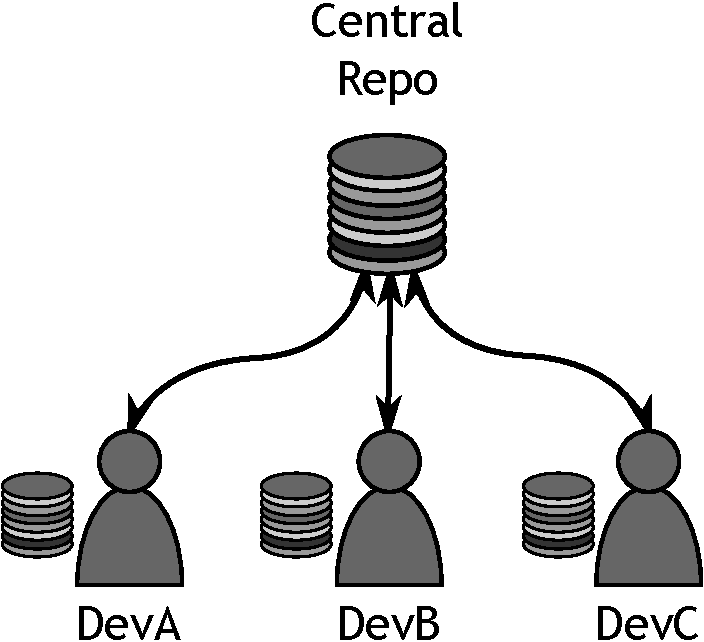
\includegraphics[width=7cm]{images/f-w1-d1.pdf}
	\caption{Centralised Workflow}
\end{figure}

\subsubsection{Integration Manager Workflow}
The integration manager workflow is similar to the centralised workflow because there is still a \textbf{blessed} repository which everyone uses as a reference.  The difference here is that there is only one person who has the rights to push changes to the \textbf{blessed} repository.  This person is referred to as the Integration Manager.  

This workflow is handled exceedingly well by Git.  Developers will work on their repositories locally and then once they are happy, will push their changes to a location where the Integration Manager can see them.  The Integration Manager will then review the changes that the developers have made and will merge them into their own local repository.  Once they are happy that everything is working well, the Integration Manager will push their changes to the blessed repository so that all the other developers can access the changes.

\begin{figure}[bt]
	\centering
	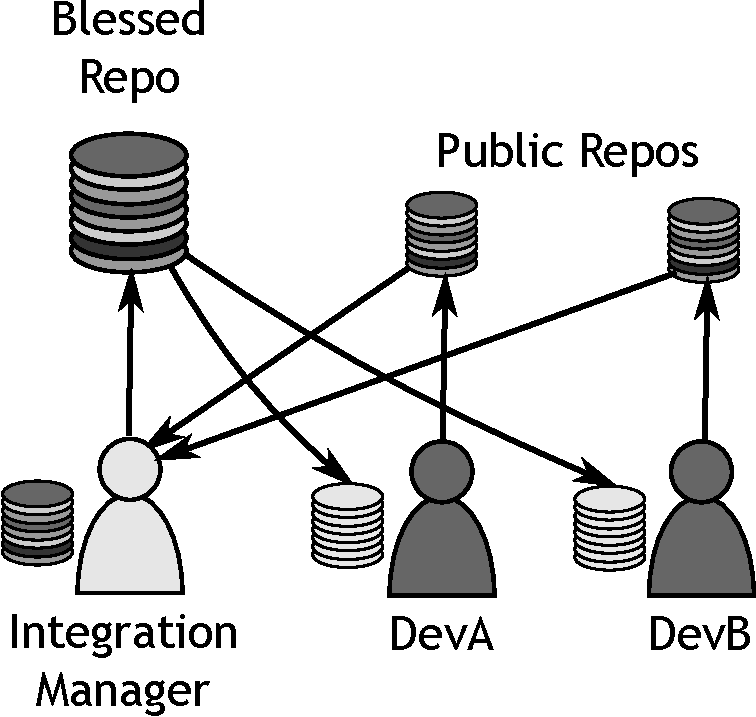
\includegraphics[width=7cm]{images/f-w1-d2.pdf}
	\caption{Integration Manager Workflow}
\end{figure}

\subsubsection{Dictator and Lieutenant Workflow}

The dictator and lieutenant workflow is practically an extension to the integration manager workflow.  It is more suited to larger teams, where modules or sections of the code can be assigned to a \textbf{Lieutenant} who is responsible for blessing all of the changes to that particular section.

Once the Lieutenants are happy with their code, they make it available to the Dictator.  The Dictator then takes on a role similar to the Integration Manager from the previous model.  In the end, all of the changes are pushed to the blessed repository for the developers at the bottom of the tree to pull from.

\begin{figure}[bt]
	\centering
	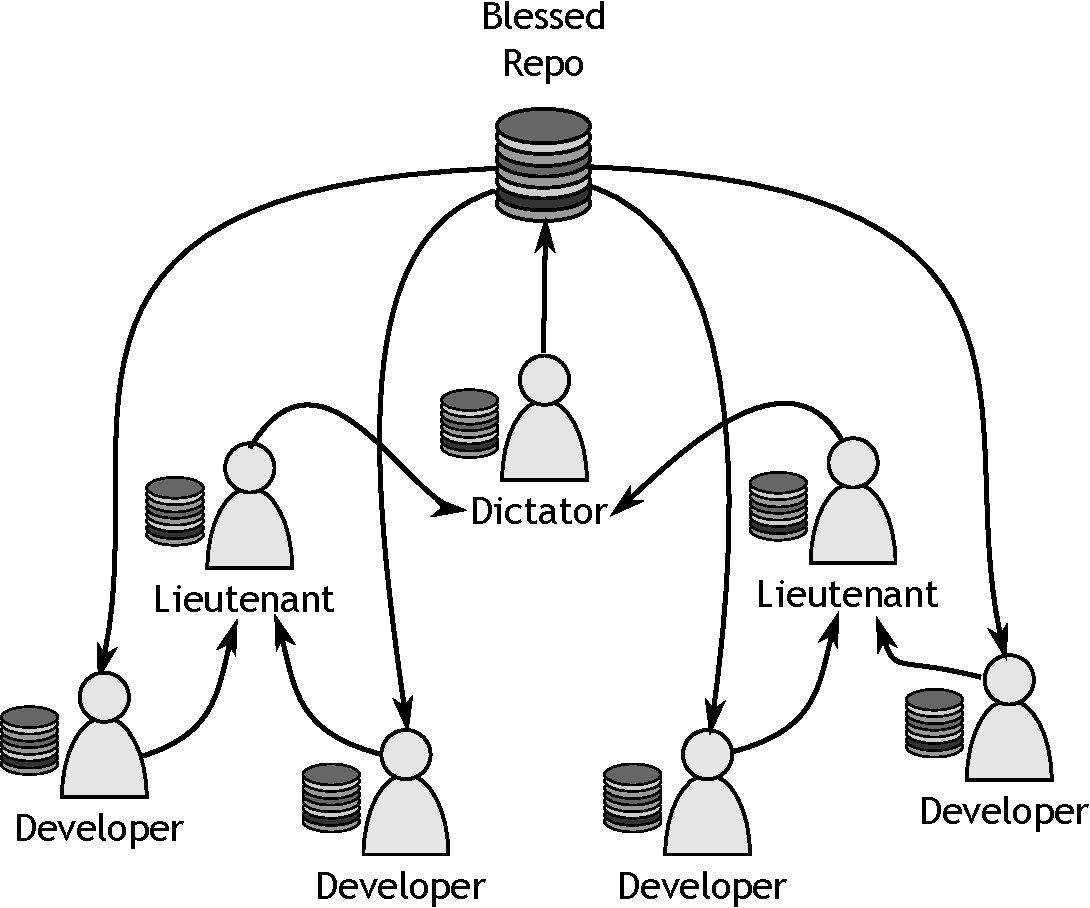
\includegraphics[width=7cm]{images/f-w1-d3.pdf}
	\caption{Dictator and Lieutenant Workflow}
\end{figure}

\begin{figure}[hbt]
\tikzstyle{mybox} = [draw=black, fill=gray!20, very thick, rectangle, rounded corners, inner sep=15pt, inner ysep=20pt]
\tikzstyle{fancytitle} =[fill=black, text=white]
\begin{tikzpicture}
\node [mybox] (box){%
    \begin{minipage}{.9\textwidth}
A blessed repository is one which has the approval of the managers of the project.  The blessed repository is supposed to be the de facto standard where all other clones are made from.  If there is one place where code should be correct, it is the blessed repository.  If you are hosting the project in a public place, the blessed repository will usually be the one that is made available to people as a stable point for developing from.
    \end{minipage}
};
\node[fancytitle, right=16pt] at (box.north west) {Blessed};
\node[fancytitle, rounded corners] at (box.west) {\rotatebox{90}{Terminology}};
\end{tikzpicture}
\end{figure}

The main thing to remember, is that Git can utilise any of these workflows.  This makes it a very flexible system, allowing you to work in whichever way you decide.

\subsection{Offline Committing}

Perhaps one of the most useful and undervalued features of version control systems is that of offline committing.  It may be undervalued because not all version control systems have it.  Offline committing is the ability to continue adding and committing files to the repository without being connected to a centralised repository.  

When travelling or just simply when out of the office, developers and integrators alike are able to continue managing code, viewing histories, viewing diffs and committing changes to their repository.  This is all due to the fact that Git does 99\% of all of it's operations locally.  When a repository is cloned, Git actually sets up a copy of the entire repository locally, giving developers the flexibility to work anywhere, without requiring access to the company network.

When returning to the office, the developers simply push their changes to their ``public'' space, be it local or to a blessed location, and all of the commits that have been made whilst they are away are then made available to the rest of the team, including all history and snapshots.

\subsection{Developer Interaction}

One factor to consider when choosing a version control system, is that of developer interaction.  By this we are referring to the way in which developers use and interact with the version control system itself.  There are four main methods for VCS interaction

\subsubsection{Graphical User Interface Client (GUI)}

A graphical user interface allows the developer, or user, to physically manipulate the repository using a mouse pointer and a graphically rich environment.  A GUI client will typically consist of separate application which is run when a user wants to make changes to a repository such as adding files or committing changes.  

Some developers prefer having a separate client with which to interact with their repository, whilst others prefer to have things integrated a little more.

\subsubsection{Shell Extension Integration}

Shell integration allows the user to interact with their repository using the graphical environment that they would usually use for manipulating files and performing routine directory maintenance.  One of the most common Shell Extensions for Git is the TortoiseGit interface which integrates itself into Windows Explorer, allowing a user to right click on an entity whilst inside a git working tree, and be presented with a context sensitive menu for VCS operations.

\subsubsection{Command Line Interface (CLI)}

The command line interface is favour by many developers as they can script with it and can see exactly what is going on, often in much more detail that with a GUI.  The CLI gives total control over the product and it is worth noting that almost all version control systems start life as command line driven interfaces.  Why is this so?  It can take a lot of time and effort to put all the options and nuances of a system into a GUI.  The CLI will almost always be the most powerful of all tools, especially where version control systems are concerned.

\section{Day 4 - ``A decision is reached''}

\subsection{Analysing Your Requirements}

The most important aspect of choosing a version control system, is to define your requirements.  These can be few, or they can be quite specific, let's see what John and his team decide are the most important aspects for them and ultimately what they decide upon.

\begin{trenches}
``Offline committing seems like it's a pretty useful thing to have.''  Mike said nodding.  ``Especially with people like John travelling all the time.''

``I have to admit, it would be nice to be on the plane, and be able to pull all the code together, knowing all of the history of each section,'' replied John.  ``The branching in Git seems to be quite powerful as well.''

``I must admit,'' chimed in Klaus, ``I've used branching a bit in Subversion before and it was a lifesaver.  It's supposed to be super fast in Git too.''

``And owing to the fact that Git seems to support several workflows, it means we can try them out and see how they work for us.''  Markus looked at the team.  ``Are we settled on Git then?''

The team nodded and everyone walked out of the board room except John.  Things were about to get interesting for him.  Very interesting.
\end{trenches}

Since this book is all about Git, we won't delve too far into the workings or features of other version control systems.  Hopefully, this chapter has given you enough information to go and check out some of the other systems, if you feel the need to.  The main thing to bear in mind is that Git is a Distributed Version Control system.  While this is so, it is equally important to remember that it can be used in the same workflow models as Centralised Version Control systems.

John and his teams requirements are nothing special.  They are a smallish team looking to reap the benefits of having their code in a well organised system.  They are also looking to reorder their team functions and dynamics in order to fit around the version control system and really make it core to their development.  

Version control is not a replacement for workflow.  It is not intended to make everything better.  If you have people going off and doing their own thing and being careless about the way they work, version control is not going to suddenly fix everything.  A tool is just that, a tool and version control is no different.  You can buy the messiest builder in the trade a nice shiny new tool box, but unless they have the mindset to want to change, you'll probably find that all the tools end up in the largest compartment at the bottom.

\section{Day 5 - ``Working like a team''}

\subsection{Team Organisation}

Now that we have the basics dealt with, let's take a little look at how John arranges his team, and see whether version control is going to work for them.  It is important that the team understands how the model should work, what they are expected to do and what level of access they have.  Most of the time people will get more frustrated about not know what they should or shouldn't be doing, rather than that they do or don't have access to certain things.

\begin{trenches}
It was 4:36pm on the Friday and the table in the board room was littered with empty coke cans, pizza boxes and one Japanese bento lunchbox, owned by a particularly stubborn member of the team who had vowed never to eat pizza again.  It had been Marcus' idea to bring in the food reinforcement to help the discussions along.  The team were trying to decide how to organise their model.

``There's nothing to say we can't use a combination of the models is there?'' asked Mike.

``I suppose not,'' said John.  ``What did you have in mind.''  His glasses were slipping down his forehead now and he was getting pretty tired.

``Well, I figure, we basically have the software split into two parts.  We have the library, which myself, Klaus and Jack work on.  Then there's the UI elements which Simon, Martha and Rob handle.  I know there are the tools which Eugene works on too.''  Everyone had started to listen to Mike as he continued.  ``John, you don't want to have to deal with the library component as this more Klaus' space.  So why don't we have two dictators.  Klaus and yourself have access to push up to the blessed repository.  John can pull from his guys, Klaus from his and we end up with an good model for version control.''

John raised his eyebrows, ``Not bad Mike,'' he said, genuinely impressed.  After spending a few hours going through the various models and who was  in charge of what, it felt good to have finally reached a decision.

``So, we start on Monday then?'' asked Markus, who had been listening from the other end of the table.  

``Indeed.''  Announced Klaus, ``Monday we all become Gits!''
\end{trenches}

% afterhours1.tex - Afer Hours Week 1
\chapter{After Hours Week 1}
\section{``History Lesson''}
\subsection{A Brief History Of Version Control}

\subsubsection{The Very Early Days}
Version control systems have been around for forty years (2011 at the time of writing).
During this time they have undergone an intense amount of change and have evolved into some of the most incredibly powerful tools utilised in software development today.
Chances are that in the early days you will have started off storing different versions of your source code and documents in separate files and folders.
You may have even archived them off to compressed storage files, like zip or tar.
Rest assured, you are not the first person to do this, and in 1972, someone called Marc J.
Rochkind, decided to create system for storing revisions of documents and source code.

The system Marc created was called SCCS and stood for Source Code Control System, in essence probably the most apt description for what we mainly use a version control system for today.
SCCS was originally written for an operating system called OS/360 MVT and was later ported to C, and was used as the most dominant version control system for UNIX, until ten years later, when RCS was introduced.

\subsubsection{Time To Move On}
In 1982, Walter F.
Tichy released RCS, standing for Revision Control System.
It was intended to be a free and off more functionality than SCCS.
RCS is still being maintained, as part of the GNU project, and at the time of writing is about to have its first new release, version 5.8, in over fifteen years.

However, RCS, like it's predecessor SCCS, has no way of dealing with groups of files.
Essentially, each file has its own repository which is stored near to the file under a different name.
Whilst rather advanced, with primitive forms of branching, the interface, commands and version numbering have been described by some as rather cumbersome.
Enter some successors.

CVS was created in 1986, and began life as a set of shell scripts to operate on multiple files, using RCS to perform the actual repository management.
As development continued, this way of working was dropped and CVS began operating on files itself, evolving into a version control system in its own right.
The current iteration of CVS was released in 1989 and on November 1 1990, version 1.0 was released to the Free Software Foundation for distribution.

CVS did not version file renames or moves at all as at the time, re-factoring - a process of modifying code to improve some non-functional attributes of the software, was often avoided and so the feature was not required.
CVS also did not support atomic commits.
An atomic commit is used by more modern version control systems to safe guard the database.
In essence atomic committing is the act of applying multiple changes in a single operation.
If any of the changes do not apply correctly, all others are reverted and the commit is aborted.
When designing CVS this was not seen as an obstacle, as it was thought by the developers that a server and network should have enough resilience that it would never crash whilst committing.

Whilst active development of CVS has apparently ceased, as of May 2008, it is worth taking note that CVS defined the model for branching that was included and refined in almost all version control systems since.

\subsubsection{Offering Commercial Support}
Now that version control was advanced enough and people had begun to rely on VCSs in general, commercial offerings began to spring up.
Three prominent systems that were released within a short time of each other and ClearCase, VSS and Perforce.
All three of these are proprietary systems which were developed and filled a gap in the market for commercially supported systems.

VSS, originally developed by One Tree Software for several platforms, was continually developed by Microsoft, who bought One Tree Software in 1994, with the one caveat that Microsoft ceased development of all VSS on all platforms other than Windows.
VSS integrated into Visual Studio, Microsoft's Integrated Development Environment.
VSS has now ceased development, but ClearCase, now developed by a division of IBM, and Perforce are still being actively developed and maintained.

\subsubsection{The Millennium}
The millennium brought with it a new breed of version control systems.
Subversion, or SVN as it is colloquially known as, was developed primarily to be a replacement and mostly compatible successor to CVS.
SVN was first released in 2000 and by 2001 was able to sufficiently host its own source code due to its own advancement.
In November 2009 Subversion was accepted into the Apache group and is currently developed and maintained by its community and by several commercial entities.

Subversion brought things to the table that previous version control systems did not.
As it was released as free software, in the same vein as CVS, it was widely adopted by the open source community and later into commercial environments for its vastly improved feature set.
For a start SVN offers true atomic commits.
This gave it a definite advantage over CVS as it was seen as a truly robust alternative.

It also brought in features like the tracking of files through renames and moves, including their entire version history and the versioning of symbolic links.
SVN moved with the times and introduced many other sought after features, such as HTTP serving, cheaper branching, efficient network operation and native support for binary files.

As with all version control systems, there are aspects that people dislike.
In Subversion, people often fine the implementation of tags - names that point to specific points in the history of a repository, an issue.
In SVN, a tag is actually a branch.
What makes this different to other systems such as Git and its predecessor CVS, which literally point to a specific commit in the tag, SVN actually creates a snapshot of the file system, albeit using cheap branching.
Whilst this is lightweight on the repository, it is incredibly heavyweight on the client.

Another issue with the tagging model in SVN is that it holds no history information.
This makes it impossible, for example, to take two tags and try to find out all logged commits that occurred from one to the other.
This is the difference between using a copy as a tag, and implementing a reference.
Tags should also be read-only implicitly by their very nature, they should refer to a point in history.
However as tags are implemented as branches in SVN this is not the case.

\subsubsection{Introducing the Linus Factor}
The Linux kernel was at one point maintained under a source control system called BitKeeper.
The decision, in 2002, to use BitKeeper for the management of the Linux kernel source was rather controversial, the main opposition being that BitKeeper was a proprietary system that was offered by BitMover.
At the time, BitMover offered certain open source projects the opportunity to use BitKeeper at no cost, so long as the community developers did not engage in the creation of a competing tool.

In April 2005, BitKeeper withdrew the free license that it had granted to the open source communities, after allegations of reverse engineering by some parties on an unrelated project.
Due to the way BitKeeper worked, and decisions made regarding licensing it became impossible for several key developers, and according to some reports including Linus himself, to actually own even a commercial version of BitKeeper.

It was due to these circumstances, that Linus Torvalds himself, decided to begin writing his own version control system that would enable him to have all of the features that he had had available to him with BitKeeper, the most important of these seemingly being a distributed environment.
Linus decided on a set of criteria, which along with a distributed environment, also included a robust safeguard against corruption, be it accidental, or malicious, and very high performance.

Git development began on the 3rd of April 2005, and by April the 7th, the project had been announced and was already able to host itself.
On June 16th, the release of the Linux kernel version 2.6.12 was managed by Git.
Junio Hamano, who had been a major contributor to the project, took over maintenance of Git in July, and by December had released version 1.0 to the community.

Interestingly enough, another project was also created as a result of this chain of events.
Mercurial or Hg as it is often known, began development on April 19th of the same year and was started by Matt Mackall with largely the same goals as Git.
Though Git was chosen to be the version control system used by the Linux kernel, Mercurial is actively used by many other projects and shares a very similar design and concept to Git.

\subsubsection{Design Changes}
Git has some features which should be discussed here as many of them are different to every other version control system.
Perhaps one of the most important of these is the very strong emphasis on non-linear development.
Git provides many tools with which to work with many branches and merges, with a core principal being that changes will often be passed around more than they will be written.

Git is very fast.
Though for certain operations it may be slower than some of its peers, Git has been consistently proven to be faster than most.
This design implementation was essential as the Linux kernel is indeed a very large project.

When developing systems that offer any kind of security to an end user, it is essential to provide a way of auditing the history of the code, to ensure that no tampering has taken place.
Due to the way that Git is implemented, each SHA-1 hash, used to identify a particular commit, depends on the entire history of the repository.
What does this mean to someone viewing the repository? Once the repository is published, it is impossible for someone to tamper with the history without someone noticing.
This is called cryptographic authentication of history.

Of course the most important feature, and one which will be discussed in great detail later in the book, is that of distributed development.
The emphasis on non-linear development and the implementation of very cheap and fast branching, makes Git one of the best version control systems on the market for distributed development.

As mentioned previously every version control system has advantages and disadvantages and it would not be fair to make out that Git was without flaws.
Some that have been mentioned by people over the years are its particular steep learning curve for basic understanding.
Whilst it is agreeable to some degree, it is largely due to the fact that Git is a distributed version control system and inherently these systems are more complex in their implementation that others.
Another bug bear of some people, is the fact that Git will not track empty directories.

\subsubsection{Wrapping Up}
Though there are many other version control systems out there that are being actively developed, such as Bazaar, Plastic and Darcs, to name but a few, we are going to end our historical tale here and continue with learning more about the Git version control system.
There is a plethora of information available on the Internet about version control, so if you want to find more information about any of the systems mentioned here, that would probably be the best place to start.

% chap2.tex - Week 2
\chapter{Week 2}
\section{Day 1 - ``We are coders, we use Git!''}
\subsection{Setting Up the Environment}

So now we are ready to begin delving into and actually using Git, right?  Well, not exactly.
First we have to decide upon how the workflow model we have envisaged is implemented in our version control system.
With Git being so versatile, it's both a blessing and a danger.
It is a good idea to define from early on, exactly how you would like the developers, lieutenants and dictators to behave, before you begin actually committing any code.
Sometimes this isn't possible.
It's quite feasible that you have never used a version control system like Git before and you begin by muddling your way through.
This is normal, but if you are in charge of implementing this type of system for a professional environment, you should really consider first how this is going to work.

Conceptually, the model which was discussed previously is easy to imagine.
We have two dictators, who both have access to the blessed repository and then several developers, who are going to have their changes reviewed and included, by the aforementioned dictators.
The physical representation of the workflow model is summarised in the diagram below.

\begin{figure}[bt]
\centering
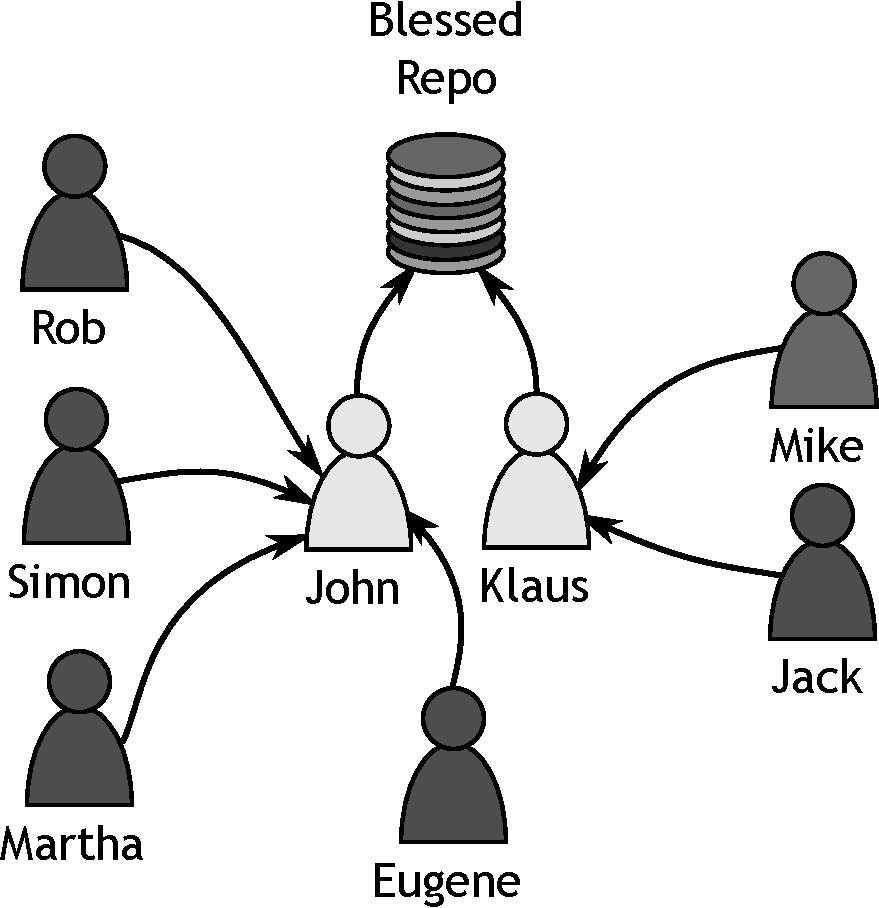
\includegraphics[width=7cm]{images/f-w2-d1.pdf}
\caption{Tamagoyaki Inc's Physical Structure}
\end{figure}

The physical structure is all well and good, but it doesn't determine exactly how the data is moved, just who is responsible for it at each stage in the process.
What is required, is a detailed analysis of where the data flows from and to.
A data flow diagram is useful, but not essential.
However, we will create a slightly different form of diagram to show how the data will be moved from one person to another.
Before we go ahead and look at the diagram, let's go back to the trenches to see how the guys are coping with their repository design.

\begin{trenches}
``John, why are we all sat in here at 9:45am on Monday morning.''  Klaus whined.
``I haven't even ingested enough coffee to check emails yet, let alone meet with people.''

John grinned, ``I don't think any amount of coffee will help you there Klaus, it's your winning personality that will pull you through.''  The rest of the team laughed and then subsided as John started drawing furiously on the board.
``So we have our physical model.
We know which people are going to be in charge of things, but we don't know yet how to arrange our repositories.''

``Good point,'' chimed Mike.

``So.
Obviously we're going to have a blessed repository,'' said John, drawing a circle on the board.
He stepped back, one hand on chin.
``Then I would imagine Klaus and I will have clones of that repository on our local machines.
We will then modify those and push our changes back up to the central copy.''

``I thought Git didn't have a central copy?'' asked Martha.
There were other moans and grunts.

``Well,'' said John, ``as far as I understand it, it doesn't.
I mean Klaus and I will have local copies of the repository too.
We will work on those and then sync our changes back to the server.
It's a sync, moreover a copy.
I think it's actually called a clone.''  He nodded to himself, ``And, since Klaus and I will hardly ever overlap on code, we shouldn't ever need to merge or deal with an conflicts.''

``But what about us monkeys?'' asked Martha, ``Where do we get our clones from?''

``From the central server of course,'' Rob stated smiling.

``Yes,'' John said, ``but I think what Martha is trying to say, is how will you get your updates?''  He started to walk around the room, and one or two of the developers followed him as he reached the windows and leant on the sill.
``I guess you would merge your branch with the blessed one.''

The room went silent and the only noise that could be heard was the rattling of the air conditioner in the ceiling above.

Simon spoke out, ``Well, I was reading over the weekend about this thing called rebase and how in some cases a rebase is better than merging.''

``What's rebase and how is it different to merging?'' asked Mike.

``Well, rebasing is pretty darn clever.
Think of it this way.
You have an upstream branch, in this case, our blessed repository.
You are happily making changes.
When the upstream changes, you could merge the changes in from blessed.
If you do this, you create a single commit which merges the changes in.
It works, but\ldots'' he trailed off a little, ``it can cause problems in certain instances.
A better way to handle it is with rebasing.
Rebasing can take all the changes you have made, squirrel them away, pull down all the changes to bring it up to date, and then whack your changes on top.''

John breathed out, ``It sounds pretty cool Simon, but one thing is abundantly clear, we need to learn more about the Git basics before we start delving into this merging and rebasing.
Let's spend the rest of the day playing with some test repositories and reconvene tomorrow.''
\end{trenches}

If you've never played with a version control system before it is a good idea to take some time to just play.
Pretty soon you'll have learnt the basics and will be in a position where you will want to put your newly honed skills into practise.
Though playing on test repositories is good, it is quite usual that you need to actually use the system in a real environment before real problems arise.
The rest of this chapter is a very quick introduction to Git.
It is presented as an introduction, because it is hoped and expected that the you will take some time out to get to know the system and how it works.

\subsection{Initialising A Repository}
The first thing we need to do is to understand two very important things:

\begin{enumerate}
  \item How to create a Git repository
  \item What a Git repository actually is
\end{enumerate}

The first of these is relatively easy to perform.

\begin{Verbatim}
john@satsuki:~$ mkdir coderepo
john@satsuki:~$ cd coderepo/
john@satsuki:~/coderepo$ git init
Initialized empty Git repository in /home/john/coderepo/.git/
john@satsuki:~/coderepo$
\end{Verbatim}

What we've done here is create a new directory called coderepo, moved into it, and then run the \indexgit{init} command.
The result of this command is a new directory in the coderepo directory called \texttt{.git}.
This directory will hold a local copy of our entire repository.
This will allow us to create branches, merge changes, rebase things and ultimately push our changes to somewhere else.

Something that is crucial to the running of a repository, whether you are an administrator of Git, or a developer who is using it, is an understanding of how Git works.
It is fine to jump in and play with the repository and test the water, but before committing to using Git in a production environment, you should understand what Git actually does in the background in some detail.

During the writing of this book several people have told me that Git is one of the only version control systems where a good understanding of how the underlying system works is not just highly recommended, but bordering on essential.

Let us take a few minutes to talk about how Git works internally and how the data is actually stored.
Git doesn't store changes to files, but actual snapshots of files at specific points in time.
It refers to these by running an \index{SHA-1}SHA-1 hash against the file.
By doing this, it is easy to Git to detect if a file has changed.
If the SHA-1 hash of a file changes, then the file must have been modified.

When a commit is made to the repository, Git stores a few things.
A \index{commit}commit object is created.
This contains information about who made the commit, the parent of the commit and points to a tree object.
The tree object describes what the repository looked like at the time of the commit.
In other words the tree object, tells Git what files were in there.
Lastly, Git stores the files that were in the repository under their SHA-1 names in the objects directory.
Of course Git is super clever here because if you have exactly the same file in multiple commits, the SHA-1 hash of that file doesn't change and therefore Git only stores one copy of the file to save space.

The commit object is also referred to by an SHA-1 hash.
This is different to many other version control systems which use either a number that refers to the repository or a per file version number.
Getting used to seeing 40 character SHA-1 hashes can take a little time.
Saying "I need the commit referred to as  bf81617d6417d9380e06785f8ed23b247bea8f6d," is certainly not as easy as saying you need revision 6.
However, Git handles these hashes well, and you can reference a commit using a few of the characters from the beginning, as long as those characters uniquely refer to that commit, i.e., as long as your choice isn't in any way ambiguous.

\section{Day 2 - ``Making commitments''}
\subsection{Let's Make a Repository}

The most simple way of committing a file into the repository is to create it, or bring it into your working copy and use the commands below.

\begin{Verbatim}
john@satsuki:~/coderepo$ touch my_first_committed_file
john@satsuki:~/coderepo$ git add my_first_committed_file
john@satsuki:~/coderepo$ git commit -m 'My First Ever Commit'
[master (root-commit) cfe23cb] My First Ever Commit
 0 files changed, 0 insertions(+), 0 deletions(-)
 create mode 100644 my_first_committed_file
john@satsuki:~/coderepo$
\end{Verbatim}

What we have done here, is to create a new blank file and add it into the repository using the \indexgit{add} command.
Then we have committed it into the repository using the \indexgit{commit} command.
Let's make a few changes to our working copy and see what the result is.
First we are going to add another two new files, then we are going to make changes to our original file and finally we are going to run git status to see what Git has to say about our changes.

\begin{Verbatim}
john@satsuki:~/coderepo$ echo "Change1" > my_first_committed_file
john@satsuki:~/coderepo$ touch my_second_committed_file
john@satsuki:~/coderepo$ touch my_third_committed_file
john@satsuki:~/coderepo$ git status
# On branch master
# Changed but not updated:
#   (use "git add <file>..." to update what will be committed)
#   (use "git checkout -- <file>..." to discard changes in
 working directory)
#
#	modified:   my_first_committed_file
#
# Untracked files:
#   (use "git add <file>..." to include in what will be
 committed)
#
#	my_second_committed_file
#	my_third_committed_file
no changes added to commit (use "git add" and/or "git
 commit -a")
john@satsuki:~/coderepo$
\end{Verbatim}

So we can see that \indexgit{status} is reporting that there are changes to our first committed file, and that our second and third files are \textbf{untracked}.
\index{untracked!files}Untracked files are ones which Git detects as being present in the working directory, but which haven't yet been added and there for upon running a commit, these files will not be added to the repository.
Notice that if we tried to run a commit now, nothing would actually be committed to the repository.
Even though there are changes to to my\_first\_committed\_file, we have not asked Git to include these.
So, let's go ahead and do that, and at the same time we'll make a few changes to my\_second\_committed\_file, and add those too.

\begin{Verbatim}
john@satsuki:~/coderepo$ git add my_first_committed_file
john@satsuki:~/coderepo$ echo "Change1" > my_second_committed_file
john@satsuki:~/coderepo$ git add my_second_committed_file
john@satsuki:~/coderepo$ git status
# On branch master
# Changes to be committed:
#   (use "git reset HEAD <file>..." to unstage)
#
#	modified:   my_first_committed_file
#	new file:   my_second_committed_file
#
# Untracked files:
#   (use "git add <file>..." to include in what will be
 committed)
#
#	my_third_committed_file
john@satsuki:~/coderepo$
\end{Verbatim}

Now we can see that one of the sections has changed to "Changes to be committed".
So this means that Git has recognised and remembered that we are expecting these files to be committed when we next run a \texttt{git commit}.

\subsection{Committing the Uncommitted}

\begin{trenches}
``John, what is going on here?'' shouted Klaus from across the hallway.
The entire office had heard Klaus banging his hands down on the desk for the last fifteen minutes.
``John!'' the shout turned into a scream.

``Calm down Klaus, I'm just coming.''  John walked over to Klaus and pulled up one of the folding plastic chairs.
After a few minutes of fumbling he finally managed to take up his position next to an infuriated Klaus.

``John, Git is driving me crazy.
I have added files to the repository and I keep running a commit, but the changes aren't getting put into the blasted repo.''  Klaus was clearly distressed and John resisted the urge make jokes.

John pointed at the screen.
``Run a git status Klaus and I'll show you what the problem is.''
\end{trenches}

To understand what Klaus was getting in a spin about, let's make a change to my\_second\_committed\_file now and see how this affects things.
Remember we have already added the file, but we haven't yet made a commit.

\begin{Verbatim}
john@satsuki:~/coderepo$ echo "Change2" >>
 my_second_committed_file
john@satsuki:~/coderepo$ git status
# On branch master
# Changes to be committed:
#   (use "git reset HEAD <file>..." to unstage)
#
#	modified:   my_first_committed_file
#	new file:   my_second_committed_file
#
# Changed but not updated:
#   (use "git add <file>..." to update what will be
 committed)
#   (use "git checkout -- <file>..." to discard changes in
 working directory)
#
#	modified:   my_second_committed_file
#
# Untracked files:
#   (use "git add <file>..." to include in what will be
 committed)
#
#	my_third_committed_file
john@satsuki:~/coderepo$
\end{Verbatim}

How interesting!  We now have three sections and one of our files appears twice under both Changes to be committed and Changed but not updated.
What does this mean?  If you remember back, we spoke about a \index{staging}staging area.
This is one area in which Git differs to many version control systems.
When you \textbf{add} a file into the repository, Git will actually make a copy of that file and move it into the staging area.
If you then go ahead and change that file, you would need to run another git add in order for Git to copy your changed file into the staging area.
The most important thing to remember is that Git will only ever commit what is in the staging area.

So, if we go ahead and run our commit now, we will only have the changes marked in Changes to be committed appearing in our repository.

\begin{Verbatim}
john@satsuki:~/coderepo$ git commit -m 'Made a few changes to
first and second files'
[master 163f061] Made a few changes to first and second files
 2 files changed, 2 insertions(+), 0 deletions(-)
 create mode 100644 my_second_committed_file
john@satsuki:~/coderepo$
\end{Verbatim}

In our examples, we have used the syntax \texttt{git commit -m 'Message'}.
This is a slightly special way of committing, it allows us to specify our commit log message on the command line.
If we wanted to, we could run the command git commit and this would open a text editor that we could use to input our commands.

Let us finish off our round of committing by using the \texttt{git commit -a} option.
This commits all of the changes to files which are already tracked.
Consequently we do not have to specify the files with \texttt{git add}, like we have had to previously.
Any file which has been modified and has previously been added to the repository, will have it's changes committed upon running that command.

\begin{Verbatim}
john@satsuki:~/coderepo$ git status
# On branch master
# Changed but not updated:
#   (use "git add <file>..." to update what will be committed)
#   (use "git checkout -- <file>..." to discard changes in
 working directory)
#
#	modified:   my_second_committed_file
#
# Untracked files:
#   (use "git add <file>..." to include in what will be
 committed)
#
#	my_third_committed_file
no changes added to commit (use "git add" and/or "git commit
 -a")
john@satsuki:~/coderepo$
\end{Verbatim}

\begin{Verbatim}
john@satsuki:~/coderepo$ git commit -a -m 'Finished adding
 initial files'
[master 9938a0c] Finished adding initial files
 1 files changed, 1 insertions(+), 0 deletions(-)
john@satsuki:~/coderepo$
\end{Verbatim}

\begin{Verbatim}
john@satsuki:~/coderepo$ git status
# On branch master
# Untracked files:
#   (use "git add <file>..." to include in what will be
committed)
#
#	my_third_committed_file
nothing added to commit but untracked files present (use
"git add" to track)
john@satsuki:~/coderepo$

\end{Verbatim}

\section{Day 4 - ``Let's do this right, not fast''}

\subsection{Uh-Oh I Think I Made A Mistake}

So now we are fairly well acquainted with adding files into the repository and performing commits.
In a short while we will learn about how to view the changes we have made and perform diffs against various objects.
Before we close out the week, we need to go back to the trenches one last time.

\begin{trenches}
``Rob, ya got a second?'' asked Mike.

``Sure, what's up?'' replied Rob from across the office.
``Gimme two secs to make this commit.''  The office went silent again whilst Rob's fingers darted across the keyboard.
``Ahh.
Damn it!'' shouted Rob.

Mike rose from his chair and walked over to Rob.
``What's up?''

``I just added a file into the staging area, but I don't want it there.''  He shook his head, ``Well not yet anyway.''

Mike chuckled, ``Sorry for interrupting dude.''

``Nah, it's OK, I just need to know how to pull this file out of the index.''

``Git reset,'' shouted a voice.
The stillness of the office was interrupted by a chair free wheeling across the floor.
The occupant of the chair was Klaus.
He seemed proud that he was finally getting to grips with things.
``You can use git reset to reset a file that's in the index.''  He grabbed at the keyboard, ``Here, lemme show you.''
\end{trenches}

The git reset is great at removing things from the index that you don't want to be there.
Of course, it can do a great many other things, but for now, let us concern ourselves with the scenario presented above.
We are working away, and have added a number of files into the index ready for committing, when we discover that we are actually not ready to commit them.
In the following example, we are going to add the file my\_third\_committed\_file and then remove it from the index.

\begin{Verbatim}
john@satsuki:~/coderepo$ git add my_third_committed_file
john@satsuki:~/coderepo$ git status
# On branch master
# Changes to be committed:
#   (use "git reset HEAD <file>..." to unstage)
#
#	new file:   my_third_committed_file
#
john@satsuki:~/coderepo$
\end{Verbatim}

Notice how my\_third\_committed\_file is now ready to be committed to repository.
The problem is we need to add something more to it before we do.
Remember that when we run the git add command, we are copying the file from our working copy to the index.
If we decide we no longer want that file in the repository, we can run the following.

\begin{Verbatim}
john@satsuki:~/coderepo$ git reset my_third_committed_file
john@satsuki:~/coderepo$ git status
# On branch master
# Untracked files:
#   (use "git add <file>..." to include in what will be
 committed)
#
#	my_third_committed_file
nothing added to commit but untracked files present (use
 "git add" to track)
john@satsuki:~/coderepo$
\end{Verbatim}

We have discarded the file which was residing in the index.
This is very important to note.
We are not moving the file from the index back into our working directory, we are literally just deleting the file from the index.
Our working copy remains unaffected.
We could run the \indexgit{reset} command without appending a file.
If we did this, all the files in the index would have been discarded.

\begin{trenches}
``So, I think we are all agreed, I'll keep a version of the repository under Git version control.
Until everyone else feels comfortable with some of the more advanced features.''  John looked around the room for any disagreements but there were none.

``Agreed John,'' said Markus, ``I'm pleased with how you guys are progressing, very pleased, but like John said, it's far better for us to take our time and to implement this correctly, than to rush it and to end up with something that we can't administrate and that we don't know how it works.''

``So next week, I want you all to start playing with diffing and logs and don't forget we have an important release due too.''  John pushed his glasses further up his nose.
``The week after that we'll start looking at branching and by then we may be at the stage where we can implement our model.''

Everyone nodded in agreement.
\end{trenches}

\begin{callout}{Knowledge}{How do we change the commit message editor?}\index{changing!commit editor}
We spoke earlier about the configuration file and how it stores information about our Git instance.
Git can use any text editor you require, even a graphical one, though the need rarely arises.
As mentioned earlier, Git has a preference lever when talking about configuration.
First and foremost it will look in the repositories own 'config' file in the .git folder.
Then, it will look in the users \texttt{\textasciitilde/.gitconfig} file.
Finally, Git will look in your distributions own global folder.

If we wanted to change the editor that Git would use to modify commit messages, we can either modify the files directly, or run a command similar to the following;

\begin{Verbatim}
git config core.editor "nano"
\end{Verbatim}

If we want the changes to apply globally, meaning it would affect all repositories we administrate as this user, unless overridden by a repository setting, we would run the following;

\begin{Verbatim}
git config --global core.editor "nano"
\end{Verbatim}

It is worth noting that you can also use the \$EDITOR environment variable to accomplish the same thing.
Many people use this in preference to the modifying the Git configuration simply because many other programs honour this setting.
\end{callout}

\index{files!moving}\index{files!deleting}\index{files!adding}Now we know how to add files into the repository.
The question is, what do we do if we need to remove a file, or even rename it.
Well, git has some commands to help with that.
\indexgit{rm} and \indexgit{mv} delete and move files respectively.
Usually when you want to remove files from the repository, or move them, this is how you will handle it, but what if you have already deleted a tracked file manually?  Well, you have two options.
You could run \texttt{git commit -a}, but remember this will commit all changes to tracked files.
You could also run a \texttt{git rm <filename>} with the name of the file you have just deleted.
Git will then push that change into the staging area ready for commit.
The same applies to moving a file

However, it is worth noting something in the way that Git handles renames.
Git does not track renames explicitly.
This means that by running the \texttt{git mv <source> <dest>} command, you are essentially running a Linux \texttt{mv} command, followed by the \texttt{git rm} on the source file and \texttt{git add} on the destination file.
Running the \texttt{git mv} command is a shorthand way of doing just that.
It is worth playing with this to ensure that you understand what is happening.
As an exercise, inspect the repository after each command so that you understand at what point Git recognises your actions as a rename.

We have run through a few basic commands in Git.
If you are familiar with version control systems, then possibly the only real difference you will have noticed is that of the staging area.
It really is powerful, and allows you to organise and prepare your commits, so that they are both meaningful and coherent.

For Tamagoyaki Inc, their plan to implement version control was far too aggressive.
Most of the members of the team had never even used a version control system.
When deciding to implement version control, it is essential to ensure that you are doing it for the right reasons.
Version control is a tool to help you to keep things in order, but remember tools are nothing without process.
It is process that is key to the order.


\clearpage
\section{Summary - John's Notes}
\subsection{Commands}
\begin{itemize}
\item\texttt{git add} - Add files into the index or staging area

\item\texttt{git commit } - Commit files into the repository, using text editor for commit message

\item\texttt{git commit -m '<Message>'} - Commit files into the repository, using the command line to supply commit message

\item\texttt{git commit -a} - Commit all tracked files into the repository that have changed, using text editor for commit message

\item\texttt{git reset <path>} - Remove file from index or staging area

\item\texttt{git status} - Show the status of tracked, changed, untracked files
\end{itemize}

\subsection{Terminology}
\begin{itemize}
\index{Terminology!Branch}\item\textbf{Branch} - A way of working on the same set of code in parallel without modifications overlapping

\index{Terminology!Commit}\item\textbf{Commit} - A group of objects and a tree in a Git repository
\end{itemize}

% afterhours2.tex - Afer Hours Week 2
\chapter{After Hours Week 2}
\section{``A Litte Of Git's Internals''}
\subsection{A Look At Plumbing}

This After Hours section is going to get a little deep.  For some of you it may be more information than you bargained for.  However, sometimes, when the worst happens, it is comforting to know that you at least have a basic understanding of what is happening under the hood.  These After Hours sections are designed to give you that knowledgee.  They are for the people who are not just satisfied with knowing that things work, but they want to know \emph{why} things work.

To start with, we are going to use the Git repository that we have been playing with in Week 2 and take a deeper look at what is actually inside a Git repository.  Let us view the directory structure, to see what has been created in the \texttt{.git} folder.

\begin{Verbatim}[frame=leftline,framerule=1mm,fontsize=\relsize{-3}] 
john@satsuki:~/coderepo/.git$ ls -la
total 52
drwxr-xr-x  8 john john 4096 2011-03-31 20:35 .
drwxr-xr-x  3 john john 4096 2011-03-31 20:28 ..
drwxr-xr-x  2 john john 4096 2011-03-31 20:22 branches
-rw-r--r--  1 john john   30 2011-03-31 20:34 COMMIT_EDITMSG
-rw-r--r--  1 john john   92 2011-03-31 20:22 config
-rw-r--r--  1 john john   73 2011-03-31 20:22 description
-rw-r--r--  1 john john   23 2011-03-31 20:22 HEAD
drwxr-xr-x  2 john john 4096 2011-03-31 20:22 hooks
-rw-r--r--  1 john john  208 2011-03-31 20:35 index
drwxr-xr-x  2 john john 4096 2011-03-31 20:22 info
drwxr-xr-x  3 john john 4096 2011-03-31 20:27 logs
drwxr-xr-x 13 john john 4096 2011-03-31 20:34 objects
drwxr-xr-x  4 john john 4096 2011-03-31 20:22 refs
john@satsuki:~/coderepo/.git$
\end{Verbatim}

\textbf{branches} - Though deprecated now, this folder stores shorthands for git pull, push and fetch commands, by creating a file, the name of which is passed to the command instead of the repository argument.

\textbf{COMMIT\_EDITMSG} - This file holds the last commit message that was displayed in the editor.

\textbf{config} - This is the main configuration file for Git.  It is the first place git looks for upon invocation.  If this file is not present, Git will inspect \texttt{\textasciitilde/.gitconfig}.  After this, Git will go to \texttt{/etc/gitconfig}.  The file holds information about the remotes, tracking branches, push configurations and many more items.

\textbf{description} - This is a simple text file which gives a description to a repository when being view via gitweb or similar.

\textbf{HEAD} - This file is a pointer to the parent commit of your current branch.

\textbf{hooks} - Scripts can be placed in here to perform operations at certain points during the commit process.

\textbf{info} - The info folder contains some additional information about the repository

\textbf{logs} - The logs folder holds various logs regarding Git's operation

\textbf{objects} - The is the directory that holds all of the actual files that are stored in the repository.  The files are named by their SHA-1 values.  Inside the folder are a number of directories which make up the first 2 characters of the SHA-1 value.  The remaining portion of the SHA-1 hash is used to name the file.

\textbf{ORIG\_HEAD} - Hold the previous SHA-1 hash that HEAD pointed to.  This allows certain operations to go back, in the case of failure. (Not present in our listing)

\textbf{refs} - This folder holds the files that files for local branches, remote branches and tags.

More files and folders will appear here during the running of the repository as you begin to start using different features in Git.

The most interesting of the folders here is the \texttt{objects} folder.  This folder as previously described holds all of the objects that are stored in the repository.  Now, what do we actually mean by objects.  As yet, we have not really defined what an object is.  We are going to look now at three types of object that Git places in this directory.  These are the commit, tree and blob objects.  We need a little more information as the names themselves do not fully describe what the item is.

\begin{itemize}
\item\textbf{commit} - A commit object is an object that describes a specific point in time.  Whenever you perform a \texttt{git commit} from the command line, what you are actually doing is creating one of these objects in the repository.  This object stores information about the committer, the date, a link to the previous commit object and most importantly a link to the tree object of the current commit.
\item\textbf{tree} - A tree object defines which files were physically included in the commit when it was added to the database.  The tree contains the name of the files that were present in the tree by recording their blob SHA-1 id and their filename.  Sub-folders of a directory will be referenced by another tree object.  In this way, a tree object will contain references to both tree objects and blob objects
\item\textbf{blob} - A blob object actually contains the data that resides inside the file.  There is one object generated per revision of a file.  However, if exactly the same data resides in two separate files, then there will only be one object created and that object will be referenced by two trees.  In this way, multiple copies of the same file, or files which have not changed through multiple revisions are not stored multiple times.  Even though Git stores a complete snapshot of the filesystem at every revison.
\end{itemize}

So, when we commit into the repository we create a commit object.  The commit objects houses links to a tree.  The tree object contains links to either blobs or trees.  Regardless, the structure of a basic repository may look something a little like Figure 1.

\begin{figure}[hbt]
\centering
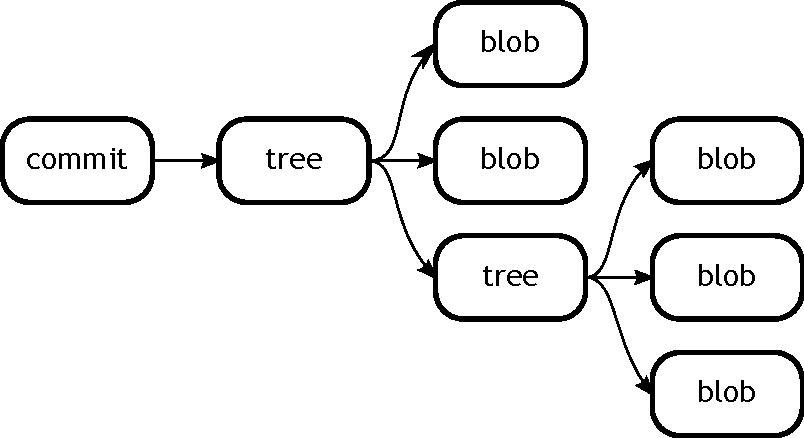
\includegraphics[width=9cm]{images/f-af2-d1.pdf}
\caption{Overview of objects in a repository}
\end{figure}

So now we know what a basic repository shuld look like, let us go through each stage of our committing in \textbf{Week 2} and see how it is built up at each stage.  Below is a consolidated list of all the objects in the repository.  

\begin{Verbatim}[frame=leftline,framerule=1mm,fontsize=\relsize{-3}]
./09/5b9cda52807c9c11781ec0a4aee927787b61f1
./16/3f06147a449e724d0cfd484c3334709e8e1fce
./34/a5dff148e70c12310cda0800d6bcaf82530bdc
./3a/d4cc3fe5a61c5563cb1b2ff3680d7e95be0fce
./3f/fa7ab6dafef2bc38a70a39c53604c333ed4d7a
./8d/664b74cce3a1f24d498d2d2bcc36e9915b5a65
./99/38a0c30940dccaeddce4bb2eb151fba3a21ae5
./cf/e23cbe0150fda69a004e301828097935ec4397
./e6/9de29bb2d1d6434b8b29ae775ad8c2e48c5391
\end{Verbatim}

In order to start rebuilding a picture of our repository, let us first find out what the first commit to our repository was.  Looking back in \emph{Week 2} we can see the following trimmed output.

\begin{Verbatim}[frame=leftline,framerule=1mm,fontsize=\relsize{-3}]
[master (root-commit) cfe23cb] My First Ever Commit
\end{Verbatim}

So we need to start with the object that begins \texttt{cfe23cb}.  Remember in the description above about the SHA-1 hashes, the first two bytes are the directory name.  We are looking for a file that starts with the characters \texttt{e23cb} and it will be in the directory called \texttt{cf}.  By George!  Looking at the list above, we can see that there is one file which fits the bill.  In fact it would be a little ambiguous if there were two.  It \emph{could} happen that we would have two SHA-1 hashes  that started with the same seven characters, but it's not likely.  The line we are interested in is listed below.

\begin{Verbatim}[frame=leftline,framerule=1mm,fontsize=\relsize{-3}]
./cf/e23cbe0150fda69a004e301828097935ec4397}
\end{Verbatim}

It would be nice if we could find out a little more about this object, and confirm that it is what we expect it to be.  to start with, let us run the linux \texttt{file} command on it, to see what it makes of it.

\begin{Verbatim}[frame=leftline,framerule=1mm,fontsize=\relsize{-3}]
john@satsuki:~/coderepo/.git/objects/cf$ file e23cbe0150fda69a004e301828097935ec4397 
e23cbe0150fda69a004e301828097935ec4397: VAX COFF executable - version 5185
john@satsuki:~/coderepo/.git/objects/cf$ 
\end{Verbatim}

The \texttt{file} command, tells us that the file is actually of \texttt{VAX COFF executable - version 5185} filetype.  This is obviously not correct.  Git stores its objects by Zlib compressing them, which is why it is difficult for the \texttt{file} command to make any sense out of them.  Later in the book, you will find out exactly how to generate your own repository from scratch, but for now, let us just understand that Git first creates a header for the content, then adds the content to the header, creates the SHA-1 hash of such data and finally Zlib compresses it to store to disk.

\subsection{Out comes the wrench}
Wouldn't it be nice if we could view the data that was inside the file simply, without having to write out own tools.  If you look through the Git man page, you will find one listed under the \textbf{Interrogation} section, called \texttt{git cat-file}.  Anyone who has spent any time with Git will know what the \texttt{cat} command does.  \texttt{cat} is used to display the contents of files.  In Git, this command is used to display the contents, type or size of a repository object, be it either of type commit, tree or blob.

\begin{figure}[hbt]
\tikzstyle{mybox} = [draw=black, fill=gray!20, very thick, rectangle, rounded corners, inner sep=15pt, inner ysep=20pt]
\tikzstyle{fancytitle} =[fill=black, text=white]
\begin{tikzpicture}
\node [mybox] (box){%
    \begin{minipage}{.9\textwidth}
You may have noticed the less than subtle references to plumbing.  Git has two types of commands.  Those that are readily available to the end user, and those that are not.  

The commands that are readily available to the end user are called Porcelain commands because they have been refined and are simple to use, think Tap and Sink.  

Commands which get a little down and dirty with the details are called Plumbing commands because they are dealing with the primative objects that make things work, think Pipes and Joints.
    \end{minipage}
};
\node[fancytitle, right=16pt] at (box.north west) {What's with all the wrenches?};
\node[fancytitle, rounded corners] at (box.west) {\rotatebox{90}{Information}};
\end{tikzpicture}
\end{figure}

If we run this plumbing command against our object, and supply the \texttt{-t} parameter, \texttt{git cat-file} will tell us the type of the object.  If we run it with the \texttt{-s} parameter, it will tell us the size.  Finally, running it with the \texttt{-p} parameter we can see what the object actually contains.  Each of these has been demonstrated below.

\begin{Verbatim}[frame=leftline,framerule=1mm,fontsize=\relsize{-3}]
john@satsuki:~/coderepo$ git cat-file -t cfe23c
commit
john@satsuki:~/coderepo$ git cat-file -s cfe23c
215
john@satsuki:~/coderepo$ git cat-file -p cfe23c
tree 34a5dff148e70c12310cda0800d6bcaf82530bdc
author John Haskins <john.haskins@tamagoyakiinc.koala> 1301599664 +0100
committer John Haskins <john.haskins@tamagoyakiinc.koala> 1301599664 +0100

My First Ever Commit
john@satsuki:~/coderepo$ 
\end{Verbatim}

Fantastic!  We now have a way of confirming the objects are what we think they are.  If we were to run the command against every file in the repository, we would end up with a list that would look something like the one below.  Notice our commit object sat in the middle.

\begin{Verbatim}[frame=leftline,framerule=1mm,fontsize=\relsize{-3}]
./09/5b9cda52807c9c11781ec0a4aee927787b61f1		blob
./16/3f06147a449e724d0cfd484c3334709e8e1fce     commit
./34/a5dff148e70c12310cda0800d6bcaf82530bdc		tree
./3a/d4cc3fe5a61c5563cb1b2ff3680d7e95be0fce		blob
./3f/fa7ab6dafef2bc38a70a39c53604c333ed4d7a		tree
./8d/664b74cce3a1f24d498d2d2bcc36e9915b5a65		tree
./99/38a0c30940dccaeddce4bb2eb151fba3a21ae5     commit
./cf/e23cbe0150fda69a004e301828097935ec4397     commit
./e6/9de29bb2d1d6434b8b29ae775ad8c2e48c5391		blob
\end{Verbatim}

Now things start to get interesting.  Did you also notice the tree SHA-1 hash mentioned when we ran \texttt{git cat-file -p}?  This is the tree object that stores the file structure.  Why don't we run the command against that file too?

\begin{Verbatim}[frame=leftline,framerule=1mm,fontsize=\relsize{-3}]
john@satsuki:~/coderepo$ git cat-file -p 34a5dff
100644 blob e69de29bb2d1d6434b8b29ae775ad8c2e48c5391	my_first_committed_file
john@satsuki:~/coderepo$ 
\end{Verbatim}

We can now see a list of all files that were present in that snapshot of the working tree.  In our case this just happens to be one file.  Using our command one last time against the object name of the file, we can see the actual contents of the file.

\begin{Verbatim}[frame=leftline,framerule=1mm,fontsize=\relsize{-3}]
john@satsuki:~/coderepo$ git cat-file -p e69de29
john@satsuki:~/coderepo$ 
\end{Verbatim}

At first glance one may consider it odd that there is nothing in there.  However, if we take a trip back in time and flick back to the first commit that we made to our repository, you will see that we never actuall put any content in our file at all.  So, the object contains nothing.  Now we can draw up a diagram of our repository after the first commit.

\begin{figure}[hbt]
\centering
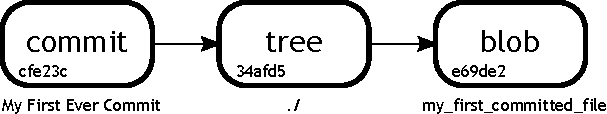
\includegraphics[width=9cm]{images/f-af2-d2.pdf}
\caption{Overview of objects in repository after \textbf{first} commit}
\end{figure}

If we pick another commit object from the list and run our command on it we can see something new has appeared in the output.

\begin{Verbatim}[frame=leftline,framerule=1mm,fontsize=\relsize{-3}]
john@satsuki:~/coderepo$ git cat-file -p 163f061
tree 3ffa7ab6dafef2bc38a70a39c53604c333ed4d7a
parent cfe23cbe0150fda69a004e301828097935ec4397
author John Haskins <john.haskins@tamagoyakiinc.koala> 1301599979 +0100
committer John Haskins <john.haskins@tamagoyakiinc.koala> 1301599979 +0100

Made a few changes to first and second files
john@satsuki:~/coderepo$ 
\end{Verbatim}

This commit object has an extra field.  This field is the \texttt{parent} field.  It tells Git which commit object is the parent to this one.  We were lucky in our guess that the parent object \textbf{cfe23cb} was actually the object we had first encountered.  By knowing this nugget of information, we can actually deduce that the object \textbf{9938a0c} was actually the next commit.  Checking in Week 2 will confirm this.  It seems we could now build a complete history of our repository so far.  If we did so, we would end up with a diagram that looked a little like the one below.

\begin{figure}[hbt]
\centering
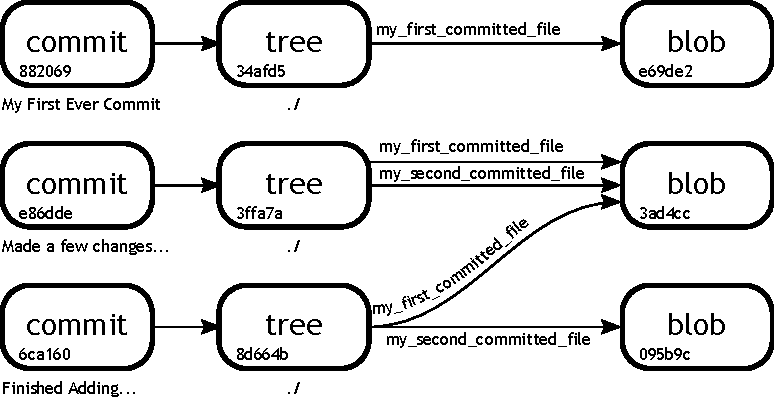
\includegraphics[width=9cm]{images/f-af2-d3.pdf}
\caption{Overview of objects in repository after \textbf{three} commits}
\end{figure}

Hopefully you can see from this diagram that Git will reuse objects as discussed above.  This diagram describes the repository layout completely and if you correlate, we have correctly identified and accounted for each object in the repository.  Now we know how to traverse a repository.  In \emph{Week 3} we find the Git commands to let us do that without having to break out the wrenches and resort to plumbing.  After all, why use a wrench to turn on a tap?

\begin{figure}[hbt]
\tikzstyle{mybox} = [draw=black, fill=gray!20, very thick, rectangle, rounded corners, inner sep=15pt, inner ysep=20pt]
\tikzstyle{fancytitle} =[fill=black, text=white]
\begin{tikzpicture}
\node [mybox] (box){%
    \begin{minipage}{.9\textwidth}
It is worth noting that the objects noted above are not the only objects that you will find in the \texttt{objects} folder.  Git will sometimes clean itself up and perform packing operations.  This is out of scope for this chapter though.
    \end{minipage}
};
\node[fancytitle, right=16pt] at (box.north west) {Packing for a holiday?};
\node[fancytitle, rounded corners] at (box.west) {\rotatebox{90}{Note}};
\end{tikzpicture}
\end{figure}

% chap3.tex - Week 3
\cleardoublepage
%\phantomsection
\chapter{Week 3}
\section{Day 1 - ``But how do I see what's going on?''}
\subsection{Logging in Git}

Perhaps the best feature of a version control system is the level of accountability that it offers if set up correctly.  What do we mean by this?  People often mistake the word \textbf{accountability} for the word \textbf{blame}.  This is not true at all.  Accountability is key in understanding the events that led up to a particular bug being introduced, or a situation occurring.  How this is dealt with, is a up to the management teams, but accountability should not be something that is revered, it should be something that is looked upon as a tool to help define the cause of a problem.

By its very nature, a version control system is also a logging system.  Every time we committed something into the repository in the last chapter, we supplied a log message.  In fact, if we don't supply a commit message, let us see what happens.

\begin{Verbatim}[frame=leftline,framerule=1mm,fontsize=\relsize{-3}] 
john@akira:~/coderepo$ git status
# On branch master
# Untracked files:
#   (use "git add <file>..." to include in what will be 
committed)
#
#	my_third_committed_file
nothing added to commit but untracked files present (use "git 
add" to track)
john@akira:~/coderepo$ git add my_third_committed_file
john@akira:~/coderepo$ git commit -a -m ''
Aborting commit due to empty commit message.
john@akira:~/coderepo$ 
\end{Verbatim}

Git will actually not allow you to commit with a blank message.  This is actually fantastic news, as people are far less likely to write a useless message than they are a blank one.  It is very important that when using a version control system you write in a useful commit message.  If you fixed a bug, say so.  If you added a new function, why not put that in too.  When someone wants to find out what a certain commit was for, or even when you come back to the project six months later and realise you've forgotten everything, log messages are crucial in piecing back together a history of development.

\begin{trenches}
``So John, I've been committing and all that,'' started Rob, ``but how do I see the history of what I have done.''

``It's really pretty simple,'' replied John, ``But it really depends on what you want to know.''
Rob placed his thumb and forefinger onto his chin.  ``Well, for now, I just want to see a list of all of my commits.''

``That one's the simplest of all.''
\end{trenches}

At its simplest, \texttt{git log} will give an output of all of the commits that have been applied to the current branch.  Depending on what type of machine you are using it on, the output from \texttt{git log} will be navigable, usually using the up and down arrows, with 'q' used to quit.  Let's have a quick look at the output of our test repository and see what the log messages look like.

\begin{Verbatim}[frame=leftline,framerule=1mm,fontsize=\relsize{-3}] 
john@akira:~/coderepo$ git log
commit 6ca160c7226731bf80973fc5bc81f6b9beda7795
Author: John Haskins <john.haskins@tamagoyakiinc.koala>
Date:   Mon Feb 21 20:59:32 2011 +0000

    Finished adding initial files

commit e86ddea25341a75275d316d8ca545aa7c73e97b3
Author: John Haskins <john.haskins@tamagoyakiinc.koala>
Date:   Mon Feb 21 20:06:57 2011 +0000

    Made a few changes to first and second files

commit 88206926cb60aed53d21ede69f9ca5b7c69cb983
Author: John Haskins <john.haskins@tamagoyakiinc.koala>
Date:   Sat Feb 19 09:23:47 2011 +0000

    My First Ever Commit
john@akira:~/coderepo$ 
\end{Verbatim}

The \texttt{git log} command shows us a chronological list of all of the commits to the repository and also gives us several more important pieces of information.  In total there are four pieces of information displayed by default.

\begin{itemize}
\item \textbf{commit} - This is the SHA-1 hash of the commit object that is stored inside the repository.  You can find more information about this in the \emph{What's inside the Git repository?} section \emph{Week 2}.  This is how we refer to the commit.  If someone asked you in what commit you \emph{Made a few changes to first and second files}, you could reply that you did that in commit e86dd.  As explained earlier, it is good to remember that you don't need to remember or type out the whole \textbf{e86ddea25341a75275d316d8ca545aa7c73e97b3}, only the first part is required.  Generally, the first five characters will do.
\item \textbf{Author} - This is the name and email address of the author of the commit.  When we begin to look at merging, you will see that the author of a commit, is not necessarily the \emph{committer} of the commit.  If you want to find out more about how to set these options, see the breakout box in this Week, called \emph{Changing your identity}.
\item \textbf{Date} - The date is simply the date at which the commit was created.  Again, note that when we start looking at merging, the date will be the date the commit was created, not the date it was merged into the repository.
\item \textbf{Commit Message} - This is the log message that was added along with the commit when it was created.  Hopefully you can now see how important it is to create useful and meaningful messages in here.
\end{itemize}

\begin{figure}[hbt]
\tikzstyle{mybox} = [draw=black, fill=gray!20, very thick, rectangle, rounded corners, inner sep=15pt, inner ysep=20pt]
\tikzstyle{fancytitle} =[fill=black, text=white]
\begin{tikzpicture}
\node [mybox] (box){%
    \begin{minipage}{.9\textwidth}
Please note, that if you are following the commits and changes on your local computer, you may not and probably will not have the same commit IDs as are presented in this book.  You are advised to use them here to follow what is happening, but to substitute them with your own values, when you start working with the rest of this chapter.
    \end{minipage}
};
\node[fancytitle, right=16pt] at (box.north west) {Note on Commit IDs};
\node[fancytitle, rounded corners] at (box.west) {\rotatebox{90}{Note}};
\end{tikzpicture}
\end{figure}

\begin{figure}[hbt]
\tikzstyle{mybox} = [draw=black, fill=gray!20, very thick, rectangle, rounded corners, inner sep=15pt, inner ysep=20pt]
\tikzstyle{fancytitle} =[fill=black, text=white]
\begin{tikzpicture}
\node [mybox] (box){%
    \begin{minipage}{.9\textwidth}
Particularly when working with other people, or when publishing your repository to a public location, it's a good idea to make sure people know who you are and how to get in contact with you.  Every time you make a commit to a repository, Git gives the opportunity to take note of who posted the commit.  When you first install Git, it probably won't have the correct information in there for you, so it's important that you take the time to set this up.

To set up your name and email address, we need to modify the \texttt{gitconfig} again.  

\begin{Verbatim}[frame=leftline,framerule=1mm,fontsize=\relsize{-3}] 
$ git config --global user.name "John Haskins"
$ git config --global user.email 
"john.haskins@tamagoyakiinc.koala"
\end{Verbatim}

That's it.  Now by default, Git will use this setting whenever you commit to a repository, unless you override it by locally modifying the repository's \texttt{.gitconfig}.
    \end{minipage}
};
\node[fancytitle, right=16pt] at (box.north west) {Changing your identity};
\node[fancytitle, rounded corners] at (box.west) {\rotatebox{90}{Note}};
\end{tikzpicture}
\end{figure}

\section{Day 2 - ``But I need more information''}
\subsection{Digging a little deeper}

\begin{trenches}
``I know John, and next time I will make a note of it, but right now, I'd really like to know where this file got changed,'' Klaus pointed at the piece of paper containing a print out, ``specifically when this function was introduced.''

John smiled.  His hands danced over the keyboard as he finished compiling an email.  ``And you've no idea when this was added at all?'' he asked.

``No, sorry John, I don't.''  He pondered, ``I guess I could write a script to untar all the versions we've created in the last week and search through them.''  He sighed, ``Can't the wonderful Git help us out here?''

A head popped up over the cubicle wall.  ``You wanna find out when a function was introduced to a file?''  It was Rob.  ``After John showed me the basics, I went and read up on it a little.  Git has some really powerful searching within the log tool.''

``Well come on then,'' blurted Klaus, ``Don't keep me hanging on.''

A chime of the popular 1966 hit sprang out in the office.

Klaus pulled a hand down over his face, ``Oh don't you all start!''
\end{trenches}

Git can actually do some rather powerful searching to assist a developer in their daily tasks.  It would have been useful if the particular item that was being searched for had been included in the log, but sometimes, things either get missed, or there are just too many changes introduced in one commit to list them all.

In these instances, the \texttt{git log -S<string>} command comes to our aid.  This command will search through the commits in a repository and will return a list of commits which introduced or removed a specific string into the repository.  First of all, let's run this against our test repository.

\begin{Verbatim}[frame=leftline,framerule=1mm,fontsize=\relsize{-3}] 
john@akira:~/coderepo$ git log -SChange1
commit e86ddea25341a75275d316d8ca545aa7c73e97b3
Author: John Haskins <john.haskins@tamagoyakiinc.koala>
Date:   Mon Feb 21 20:06:57 2011 +0000

    Made a few changes to first and second files
john@akira:~/coderepo$ 
\end{Verbatim}

You can see that \texttt{git log} has shown us the commit that instantiated the change.  As you can imagine, when using a large code base, this tool can be invaluable.  It allows us to pinpoint a specific moment when a certain string of text entered the repository.  When running this against a very large repository, this could take a long time, and so the ability to shrink the search scope down will result in a much faster result.  To do this we can append a path to our previous command.  

\begin{Verbatim}[frame=leftline,framerule=1mm,fontsize=\relsize{-3}] 
john@akira:~/coderepo$ git log -SChange2 my_first_committed_file
john@akira:~/coderepo$ git log -SChange2 my_second_committed_file
commit 6ca160c7226731bf80973fc5bc81f6b9beda7795
Author: John Haskins <john.haskins@tamagoyakiinc.koala>
Date:   Mon Feb 21 20:59:32 2011 +0000

    Finished adding initial files
john@akira:~/coderepo$ 
\end{Verbatim}

If you remember from our committing back in Week 2, we added the string \texttt{Change2} to the second file but not the first.  So the first time we run this command, it fails, as we are searching against \texttt{my\_first\_committed\_file}.  The second time we run it, we are searching against \texttt{my\_second\_committed\_file} and this is where we see a result.  Commit 6ca16 contains the commit we are looking for.

\section{Day 3 - ``What actually changed?''}
\subsection{Doing the diff dance}

Knowing what the committer thinks they committed is brilliant.  However, sometimes it's just not enough.  The reason for this is stated fairly precisely in the first sentence of this paragraph, so let us add a little formatting to bring out the real meaning.  Knowing what the committer \emph{thinks} they committed is brilliant.  By looking at the commit message we only know as much as the committer wants us to.  If they are the helpful sort, this will probably be all that we need, most of the time.  On the other hand there is always the situation where you'd like to know a little more about what was actually placed into the repository.

The \texttt{git diff} command can show us exactly that.  For more information about diff in general, see the diff breakout box in this chapter.  Think of a diff as an easy way of looking at the differences between two files, surrounded by a little context.  This can often be enhanced by a visual diff viewer, but for now, let's stick with our simple text based \texttt{git diff}.  

If we want to find out what the changes are between our current commit and one of the previous ones, we can write a command like the one below.  Notice that below, \textbf{e86dd} refers to the second commit that we made to the repository.  

\begin{Verbatim}[frame=leftline,framerule=1mm,fontsize=\relsize{-3}] 
john@akira:~/coderepo$ git diff e86dd
diff --git a/my_second_committed_file b/my_second_committed_file
index 3ad4cc3..095b9cd 100644
--- a/my_second_committed_file
+++ b/my_second_committed_file
@@ -1 +1,2 @@
 Change1
+Change2
john@akira:~/coderepo$ 
\end{Verbatim}

What this is telling us, is that between \textbf{e86dd} and our current commit \textbf{6ca16}, we added the line \emph{Change2} to the file \texttt{my\_second\_committed\_file}.  We can see this by the preceding \texttt{+} on the line \texttt{Change2}.  Let's make a few changes to our repository and see how the diffs look.  We're actually going to make a few changes to the files using a text editor so that you can't see what we've done.  Then, hopefully, when we run the \texttt{git diff} you'll be able to see clearly what has happened.

\begin{Verbatim}[frame=leftline,framerule=1mm,fontsize=\relsize{-3}] 
john@akira:~/coderepo$ git log HEAD~1..HEAD
commit fa65f06cc62291bb0cd47aef9e05953d6655fc8e
Author: John Haskins <john.haskins@tamagoyakiinc.koala>
Date:   Tue Mar 1 21:17:57 2011 +0000

    Messed with a few files
john@akira:~/coderepo$ 
\end{Verbatim}

The command \texttt{git log HEAD\textasciitilde1..HEAD} tells Git to show us the git log for all commits between \texttt{HEAD~1} and \texttt{HEAD}.  The notation used here is something new to us, but seeing as HEAD points to the most current commit, HEAD~1 points to the commit previous to HEAD.  This is how we tell Git to show us only the most recently commit.  

As it turns out, John Haskins didn't really create a very meaningful log message.  \emph{Messed with a few files} is pretty unhelpful in the grand scheme of things.  So let's be thankful that this isn't Tamagoyaki Inc's core repository and take a look at what actually happened in the commit \textbf{fa65f}.

\begin{Verbatim}[frame=leftline,framerule=1mm,fontsize=\relsize{-3}] 
john@akira:~/coderepo$ git diff HEAD~1..HEAD
diff --git a/my_second_committed_file b/my_second_committed_file
index 095b9cd..c9887f8 100644
--- a/my_second_committed_file
+++ b/my_second_committed_file
@@ -1,2 +1 @@
-Change1
-Change2
+Changed this file completely
diff --git a/my_third_committed_file b/my_third_committed_file
new file mode 100644
index 0000000..5d27866
--- /dev/null
+++ b/my_third_committed_file
@@ -0,0 +1 @@
+Addition to the line
john@akira:~/coderepo$ 
\end{Verbatim}

As you can see, we have several things going on here, so let's take each of them in isolation and see what is going on.  We are going to dissect the diff to see what each section means.

\begin{Verbatim}[frame=leftline,framerule=1mm,fontsize=\relsize{-3}] 
diff --git a/my_second_committed_file b/my_second_committed_file
\end{Verbatim}

This first line tells us that we are dealing with \texttt{my\_second\_committed\_file}.  This is showing that we are comparing the first revision, or a, against the second revision, b.

\begin{Verbatim}[frame=leftline,framerule=1mm,fontsize=\relsize{-3}] 
index 095b9cd..c9887f8 100644
\end{Verbatim}

This second line actually tells us the beginning of the object IDs, as they are stored in the repository.  Note that these IDs are not the commit IDs, but the actual blob IDs that Git uses to refer to the file.  For more information on this, checkout the \emph{Object's living in harmony} breakout box.

\begin{Verbatim}[frame=leftline,framerule=1mm,fontsize=\relsize{-3}] 
--- a/my_second_committed_file
+++ b/my_second_committed_file
\end{Verbatim}

The next few lines are telling us which is the original file, and which is the new file, so we can use this as a reference.

\begin{Verbatim}[frame=leftline,framerule=1mm,fontsize=\relsize{-3}] 
@@ -1,2 +1 @@
-Change1
-Change2
+Changed this file completely
\end{Verbatim}

Now we see some lines which are generally referred to as a hunk.  The hunk has two important pieces of information.  Section \texttt{-1,2} tells us that in the original file, we are looking at the original file (\texttt{-}), that the starting line where the change takes place is line 1 (\texttt{1}) and that the hunk applies to two lines (\texttt{2}).  The next section tells us that in the new file, the change takes place as line 1, and because the comma and remaining number are omitted, we can infer that the hunk applies to only 1 line.

The three following lines show what actually took place.  Strings \texttt{Change1} and \texttt{Change2} were deleted from the file, whereas \texttt{Changed this file completely} was added to the file.

Looking at the next diff segment, we can see it applies to a different file.  Essentially this hunk is no different to the last, the only interesting portion is shown below.

\begin{Verbatim}[frame=leftline,framerule=1mm,fontsize=\relsize{-3}] 
new file mode 100644
index 0000000..5d27866
--- /dev/null
+++ b/my_third_committed_file
\end{Verbatim}

This shows us that \texttt{my\_third\_committed\_file} is actually a new file.  Notice the \texttt{/dev/null} and the \texttt{0000000} object ID, indicating that there was no original file.

\subsection{Diffing Over A Range}
All the operations that we have performed so far have been on one commit.  Whilst important and valuable, it may be that you want to see an entire range of changes.  

\begin{trenches}
``I'm still not entirely convinced about this John,'' said Martha.  ``I've been playing around with Git, like you asked me, but it still just seems like we're replicating the work that we used to do with the readme changelogs and the tarball files.''

She sat down on a near-by chair and wheeled it over to John's desk.  She surveryed the desk for an inch of vacant real estate before finally resting her elbow on the corner of his desk next to a copy of Pro Git.

``Well, actually Martha, I can see exactly what you mean.  Up until now, there is no difference between the old and the new process.  I'm still in control of all the versions, so nothing has really changed.''  He thought long and hard, ``Tell ya what.  Why don't you give me an operation that you've always wanted to do against our code tree tarballs easily.''

``Easy,'' she snapped back, ``I want to know what changes were made for the last two weeks whilst I had been away on holiday.'' She smiled an almost mischievous smile as she referenced 'The Incident', as it had become known throughout the office.

``Easy,'' John quipped, mimicking her mannerisms.  The two broke out in laughter.  ``We can use git log for that, and I think there are some date options too.  Let me check the man page.''
\end{trenches}

Looking at the man page for git log is a mind trip for the uninitiated.  Weighing in at over 600 lines of text, it is abundantly clear that this tool does a whole lot more than viewing a simple history of commits to the repository.  It is well worth taking the time to read through the current available options by typing \texttt{man git log} on the command line.  If you have the documentation installed, this will yield the \emph{man} page for \texttt{git log}.

Listing all commits in our repository is useful, being able to filter this output is fantastic.  This is one area in which the developers of Git have placed a great deal of time and effort.  For example, we can use \texttt{git log} to not only show us the commit message, but also provide a diff output as well.  This means that for each commit entry in the output, we will see a diff as well.  Now, whilst we are further empowered by having the diff output in chronological order for each commit, we can take things further by filtering the commits.  

Suppose we want to view all the commits that we made in the last week, typing the following into the command line in our test repository yields the following result.

\begin{Verbatim}[frame=leftline,framerule=1mm,fontsize=\relsize{-3}] 
john@akira:~/coderepo$ git log -p --since="last week"
commit fa65f06cc62291bb0cd47aef9e05953d6655fc8e
Author: John Haskins <john.haskins@tamagoyakiinc.koala>
Date:   Tue Mar 1 21:17:57 2011 +0000

    Messed with a few files

diff --git a/my_second_committed_file b/my_second_committed_file
index 095b9cd..c9887f8 100644
--- a/my_second_committed_file
+++ b/my_second_committed_file
@@ -1,2 +1 @@
-Change1
-Change2
+Changed this file completely
diff --git a/my_third_committed_file b/my_third_committed_file
new file mode 100644
index 0000000..5d27866
--- /dev/null
+++ b/my_third_committed_file
@@ -0,0 +1 @@
+Addition to the line
john@akira:~/coderepo$ 
\end{Verbatim}

Notice we get to see the diff that was presented before when we ran our \texttt{git diff HEAD\textasciitilde1..HEAD} command, but this time, as we have used the git log command instead, we get to see the diff output as well.  This is what the \texttt{-p} flag is for.  Take note of the way we have specified the time period that we are interested in.  The section \texttt{--since="last week"} tells Git to filter the output and show only the entries that were committed within the last week.

This type of filtering can be exceedingly useful to a developer.  Often when problems arise, you do not have a defined point in time that you know it was last working.  However most of the time, you can say with some certainty, ``I know it was working two weeks ago''.  Using the methods described above, will give the user all of the changes, categorised by commit, that occurred in those two weeks, allowing them to narrow down the scope of exactly where to begin looking for the offending changes.

If the developer can further categorise the issue, such as, ``I know which file the change must have occurred in'', then the following example will demonstrate just how easy it is to filter the results even further.  Even in the simplified example repository that we have been using, running this command filters the output to a single file.

\begin{Verbatim}[frame=leftline,framerule=1mm,fontsize=\relsize{-3}] 
john@akira:~/coderepo$ git log -p --since="last week" -- 
my_second_committed_file
commit fa65f06cc62291bb0cd47aef9e05953d6655fc8e
Author: John Haskins <john.haskins@tamagoyakiinc.koala>
Date:   Tue Mar 1 21:17:57 2011 +0000

    Messed with a few files

diff --git a/my_second_committed_file b/my_second_committed_file
index 095b9cd..c9887f8 100644
--- a/my_second_committed_file
+++ b/my_second_committed_file
@@ -1,2 +1 @@
-Change1
-Change2
+Changed this file completely
john@akira:~/coderepo$ 
\end{Verbatim}

See how easy that is.  Note, the \texttt{--} is necessary to tell Git the following string is a path.  We no longer have the information for \texttt{my\_third\_committed\_file} present in the output.  We have filtered everything out but the information we are looking for.  When you are up against deadlines, pouring through pages and pages of diffs and changes can be incredibly time consuming.  Having the tools available to cut that output down to just the relevant material can be life saving.

\section{Day 4 - ``Finding a good reference point''}
\subsection{Tag you're it!}

During software development, a project will generally get to a point where it is ready to be released to people outside of the development team.  When this grand day occurs, it is crucial that both the developers and the users have a reference point with which to refer to the state of the code.  Having a code name or a version number means that within a very short period of time, both parties can converse about a problem, safe in the knowledge that they are on the same page.

In most version control systems, the word tagging is used to describe a reference point in the code's history.  A tag will usually refer to a single commit and labels that particular commit with a name that is easier to remember than a standard version number or SHA-1 hash.  The tag name used can be a codename, or a version number.  Often people will follow a simple numbering scheme, like \texttt{v1.9}.  

In this example, the \texttt{1} may refer to the major version number, and will denote a family of versions, often only changing a few times in a projects lifetime.  The \texttt{9} is a minor version number and can refer to a much more frequent release schedule.  You may also see textual items being appended to this version string, like \texttt{rc}, \texttt{b}, and \texttt{a}, denoting \emph{Release Candidate}, \emph{Beta} and \emph{Alpha} respectively.

Git implements tags in a very elegant way.  A tag is simply a label in Git that points to a single commit object.  The tag name can then be used in place of the SHA-1 to refer to a point in the repositories history.  Due to the simplicity of tags, it is also possible and very simple to tag a commit that occurred way into the past.  Let us take a look at a simple tag example.  We will make the current point in the repository \texttt{v1.0a}.

\begin{Verbatim}[frame=leftline,framerule=1mm,fontsize=\relsize{-3}] 
john@akira:~/coderepo$ git tag v1.0a
john@akira:~/coderepo$ 
\end{Verbatim}

On its own, this doesn't really tell us much, but running the following, shows us a little more information

\begin{Verbatim}[frame=leftline,framerule=1mm,fontsize=\relsize{-3}] 
john@akira:~/coderepo$ git rev-parse v1.0a
fa65f06cc62291bb0cd47aef9e05953d6655fc8e
john@akira:~/coderepo$ 
\end{Verbatim}

By running the \texttt{git rev-parse} with the tag name \texttt{v1.0a}, Git has returned us the SHA-1 hash of the commit we were referring to.  If we look back up at the earlier output, we can see that the most recent commit into the repository was indeed \textbf{fa65f06cc62291bb0cd47aef9e05953d6655fc8e}.  To give us something to work with, let's tag the commit \textbf{e86dd\ldots} with the tag name \texttt{v0.9}.

\begin{Verbatim}[frame=leftline,framerule=1mm,fontsize=\relsize{-3}] 
john@akira:~/coderepo$ git tag v0.9 e86dd
john@akira:~/coderepo$ 
\end{Verbatim}

Now, we can do the following;

\begin{Verbatim}[frame=leftline,framerule=1mm,fontsize=\relsize{-3}] 
john@akira:~/coderepo$ git diff v0.9..v1.0a
diff --git a/my_second_committed_file b/my_second_committed_file
index 3ad4cc3..c9887f8 100644
--- a/my_second_committed_file
+++ b/my_second_committed_file
@@ -1 +1 @@
-Change1
+Changed this file completely
diff --git a/my_third_committed_file b/my_third_committed_file
new file mode 100644
index 0000000..5d27866
--- /dev/null
+++ b/my_third_committed_file
@@ -0,0 +1 @@
+Addition to the line
john@akira:~/coderepo$ 
\end{Verbatim}

Notice that instead of using the dynamic reference HEAD, we have now used the tag names \texttt{v0.9} and \texttt{v1.0a} to refer to our previous commits and have returned the combined diff output of all the changes which occurred between the two.

You can find out more about tags and how to specify more information in the {After Hours Week 3} section at the end of this Week.

\begin{figure}[hbt]
\tikzstyle{mybox} = [draw=black, fill=gray!20, very thick, rectangle, rounded corners, inner sep=15pt, inner ysep=20pt]
\tikzstyle{fancytitle} =[fill=black, text=white]
\begin{tikzpicture}
\node [mybox] (box){%
    \begin{minipage}{.9\textwidth}
Tags are great and you should most definitely use them in your repositories to make good reference points, but there is one point that you should always remember.  Though we have not yet delved into the realms of remote branches, it is important to note that once you have tagged a certain commit, and pushed that to the repository, you cannot then remove that tag if someone else clones, or pulls your tags from that remote branch.  This will all become clearer during the next week, but fits in with the overall ethos of working with version control systems, if someone has seen the past, you should not EVER change it.
    \end{minipage}
};
\node[fancytitle, right=16pt] at (box.north west) {A little about tags};
\node[fancytitle, rounded corners] at (box.west) {\rotatebox{90}{Note}};
\end{tikzpicture}
\end{figure}

\section{Day 5 - ``Putting things back the way they were''}
\subsection{Revert, I say.  Revert!}

Whilst working with your repository, something occurs quite often, is the need to go back in time, either temporarily or permanently, or even partially.  Git allows you to do this in a multitude of ways.  Let's see a real life situation where this need could arise.

\begin{trenches}
``No, I don't have a copy of the file.  I was stupid and after I submitted it to you I er\ldots\deleted it''.  

John gave Michael the raised eyebrow look.  It wasn't the first time Michael had come to him with a similar problem.  Usually John would have had Michael go rooting through the archives to find it.  This time though, he wondered if Git might just come to the rescue.

``Tell ya what Michael,'' he grinned, ``Since this isn't the first time you've come to me with this kind of predicament, why don't you go and find out how to use Git to get the file back.''  Michael sighed.  ``I have tagged the repo each time we created an archive, so tell me what I need to run to extract it.''

\begin{center} * * * \end{center}

``Man'', started Michael running over to John's desk forty five minutes later.  ``I never knew there were so many ways to skin a cat''

Michael was a little out of shape and though he had only crossed a minor distance, he now stood there, leaned over John's desk ever so slightly out of breath.

``So, you learn much?'' asked John.

``Where d'ya want me to start?''

\end{trenches}

Where exactly do we start?  Well one of the neat things about Git is that there are many ways to produce the same result.  While that may not seem like a benefit now, the trick is knowing just how to use each tool and what the benefit is of each method.  Right now, we are ready to look at four methods for achieving the task of viewing old information in the repository.  So how do we choose which method we wish to use?  We need to answer a few more questions before we are ready to decide.

The table below shows the three methods that we have access to now.  Note that this may not be a definitive list of methods, but that these can give us access to the data we need to view.  The columns are requirements or criteria.  We need to evaluate each command in order to determine which one is right for us.  Once you have been using Git a while, these kind of evaluations will become second nature to you, but right now, we will take a look at all available options, just to see what is out there.

\begin{table}
\begin{center}
  \begin{tabular}{ | l | l | l | l | l | l |}
    \hline
    Method Name & 
    \rotatebox{90}{Alters Repository} & 
    \rotatebox{90}{Changes History} &
    \rotatebox{90}{Alters Working Copy} & 
    \rotatebox{90}{Reversible} & 
    \rotatebox{90}{Multiple Files} \\ \hline
    Reset & Possibly & Possibly & Possibly & Possibly & Yes\\ \hline
    Checkout & No & No & Yes & No & Yes\\ \hline
    Show & No & No & No & N/A & No\\ \hline
  \end{tabular}
\end{center}
\end{table}

Let's take a look at each of these in turn.  We are going to be covering two new commands and revisiting an old one.  Let us start with \texttt{git reset}.  We have already met this tool once.  When we used it previously, its purpose was to pull files out of the index that we were not ready to commit.  We were using \texttt{git reset} in its simplest state.  Actually Git can perform several other kinds of reset.  It should be noted here that using this can be quite dangerous as it can affect your index, your working copy, your branch and the pointer HEAD.  

In order to use \texttt{git reset} in any sane way to achieve our goal, we would need to look at branching, which at the moment, we are not ready to do.  In short \texttt{git reset} can drastically effect your working copy, affecting multiple files, and before we begin investigating, we really need to learn how to play in a safe environment.  

The next method on our list to discuss is the \texttt{git checkout} command.  This command can be used to bring back either a single file or multiple files and once again at this stage, is best employed in conjunction with branches.  At this point, you may be wondering why we are placing such emphasis on the use of branches.  As you will see next week, branches are incredibly powerful things, which allow you to experiment and play with your data, without the risk of losing anything.  \texttt{git checkout} will pull files from a previous commit into our working copy.  This is something remember.  If we have any changes in our working copy, the checkout will fail.

The last method we can use to view data which was in a previous commit, is the \texttt{git show} command.  This command literally pulls data from a previous version and dumps it to the standard output, a little like the \texttt{cat} command present in almost every single *nix environment.

Now that we have taken a quick look at our three methods, we must decide which one is going to be the most useful to us.  Looking at the scenario above, we can deduce that we really only need to pull out one file.  If our intention was to do large amounts of work on an old branch and pull many files from it, \texttt{git reset} may have been a good choice.  As we are looking for only a single file, we should consider looking at the checkout and show tools.

So now let us see how we can use \texttt{git checkout} to take one of our files back to the past.

\begin{Verbatim}[frame=leftline,framerule=1mm,fontsize=\relsize{-3}] 
john@akira:~/coderepo$ git status
# On branch master
nothing to commit (working directory clean)
john@akira:~/coderepo$ git checkout v0.9 -- my_second_committed_file
john@akira:~/coderepo$ cat my_second_committed_file 
Change1
john@akira:~/coderepo$ git checkout HEAD -- my_second_committed_file
john@akira:~/coderepo$ cat my_second_committed_file 
Changed this file completely
john@akira:~/coderepo$ 
\end{Verbatim}

\begin{Verbatim}[frame=leftline,framerule=1mm,fontsize=\relsize{-3}] 
john@akira:~/coderepo$ git status
# On branch master
nothing to commit (working directory clean)
john@akira:~/coderepo$ git checkout v0.9 -- my_second_committed_file
john@akira:~/coderepo$ git status
# On branch master
# Changes to be committed:
#   (use "git reset HEAD <file>..." to unstage)
#
#	modified:   my_second_committed_file
#
john@akira:~/coderepo$ git checkout HEAD -- my_second_committed_file
john@akira:~/coderepo$ git status
# On branch master
nothing to commit (working directory clean)
john@akira:~/coderepo$ 
\end{Verbatim}

Notice how we first checked that we didn't have any local modifications by running the \texttt{git status} command.  Then we are safe to run the \texttt{git checkout} command.  We used the \texttt{v0.9} tag from earlier to refer to an earlier commit state.  The next part of the command is the double hyphen (\texttt{--}) that tells Git that what comes after it is the path.  Finally we choose \texttt{my\_second\_committed\_file} as the source file.  After this, when we \texttt{cat} the file, we see that it has changed to what it used to be in \texttt{v0.9}.

We then switch the file back to the latest version by using the \texttt{HEAD} reference.  Note that on the odd occasion, the \texttt{HEAD} reference doesn't always point to where you think it does, but this is an area we are yet to cover.  Then we run the command one more time, but this time we intersperse it with a \texttt{git status} to see that there are changes made to out local working copy.

\subsection{Show me the money}
The \texttt{git show} command will have largely the same effect, except it grabs us the data without having to change existing files in our working copy.  Let us view a quick example.

\begin{Verbatim}[frame=leftline,framerule=1mm,fontsize=\relsize{-3}] 
john@akira:~/coderepo$ git show v0.9:my_second_committed_file
Change1
john@akira:~/coderepo$ git show v0.9:my_second_committed_file > temp_file
john@akira:~/coderepo$ cat temp_file 
Change1
john@akira:~/coderepo$ 
\end{Verbatim}

The format of the \texttt{git show} command is rather similar to the checkout command we used a few moments ago.  The only difference is the presence of the colon, instead of the double hyphen.  Notice how the effect of the first command is just to print out the contents of the requested file to the screen.  With the Linux environment it is easy to pipe this output to a new file.  In the example above, we pipe the output using the \texttt{>} character to the file called \texttt{temp\_file}

Hopefully you can now see that there are often several ways to achieve the same result and it is important to ensure that you choose the right tool for the job.  The reset command was too dangerous to use, the checkout command modified our working copy, but the show tool allowed us to create a new file, guaranteeing that our working copy remained untouched.

\begin{trenches}
``So, if I am currently have changes to the file you want, in my local repository,'' began John, ``What command would you recommend I use?''

Michael paused, clearly considering each method in his head.  The noise from the sandwich van's horn rang through the office and Michael immediately stood bolt upright and looked panicked.  ``The van John'' he stuttered, ``The van''

``You can go to the van when you tell me which command I should use.''  John smirked.  Michael was one of the more junior members of the team and the managers often took the opportunity to haze him.

``I'm gonna go with git show,'' he said in a rush.

``Why?'' asked John.

``So you don't harm the working tree.'' replied Michael smoothly, already walking out the door.

``You could have also branched,'' shouted Rob, who was a few steps ahead of him.

\begin{center}* * *\end{center}

``So, what's the status then John?'' asked Markus.

John pressed a button on his laptop and the slideshow on the screen advanced to show an organisational model.  ``Well, we've not had a whole lot of time this week as the release for project Manta, but we've managed to look at logging and diffing, which is something that we really needed to cover.  Klaus also showed everyone how to tag things and went through our version numbering system again as several people had forgotten.''  Everyone in the room looked at Jack.  ``We also found out about how to pull older versions out of the repository in a variety of ways.''

Markus looked pleased, ``So, what's next?''

``Klaus?'' asked John.

``Next, John put my team in charge of defining and teaching everyone about branching and merging.  This is the really important stuff.''  Klaus took over control of the laptop and clicked onto the next slide, which detailed a list of features.  ``We really need to get a good handle on these topics to be successful.  It is key to collaboration''

``Well done team,'' ended Markus, ''Wayne is going to be impressed with this.''

\end{trenches}

We now have a good working knowledge of how to do many key things in Git.  Logging and diffing is supremely important for inspecting what changes have occurred in the repository.  Though the options here are not an exhaustive list, they should give you a basic understanding of how to use the tools.  It is well worth looking at the man pages for these commands to get an idea of just how expansive they can be.  For example, the diff tool can not only show you differences between your working copy and the index, but also between your index and the latest commit, using the \texttt{cached} option.

Next we move on to branching and merging.  Branching can be a tricky subject, so it is important to understand what is happening at the repository level.  It would be prudent to look over the After Hours section for Week 2 before continuing as some of the terminology may be a little confusing otherwise.

\clearpage

\section{Summary - John's Notes}
\subsection{Commands}
\begin{itemize}
\item\texttt{git log} - Return a navigable list of commits to a repository

\item\texttt{git log -S<string>} - Show all commits that either introduced or removed a particular string from the repository

\item\texttt{git log -S<string> <path>} - Show all commits that either introduced or removed a particular string from the repository, but restrict the search to a specific path

\item\texttt{git log HEAD\textasciitilde1..HEAD} - Show all commits between HEAD~1 and HEAD, essentially the last commit

\item\texttt{git diff HEAD\textasciitilde1..HEAD} - Show the actual differences between HEAD~1 and HEAD

\item\texttt{git tag <name>} - Create a tag with the given name

\item\texttt{git tag <name> <commit>} - Retrospectively tag a commit with a given name

\item\texttt{git rev-parse <tag>} - Show the commit SHA-1 hash object referred to by the given name
\end{itemize}

\subsection{Terminology}
\begin{itemize}
\item\textbf{Branch} - A way of working on the same set of code in parallel without modifications overlapping

\item\textbf{Diff} - Shows the actual differences between files

\item\textbf{Hunk} - A section of a diff output
\end{itemize}

%git log -p
%DIFFs
%Patching

%git show master:<path>
%git diff -- stylesheet.css master:stylesheet.css
%git checkout -b <branch>

%SUBMODULE

% afterhours3.tex - Afer Hours Week 3
\chapter{After Hours Week 3}
\section{``A Closer Look At Diffs and Tags''}
\subsection{The Diff Utility}

We learnt in \emph{Week 3} how to work with a diff, and what a diff actually represents.  It is interesting to note how old the \texttt{diff} utility actually is and how it works.  The diff algorithm was developed in the early 1970s and the research published in 1976, by Douglas McIlroy, who wrote the original diff utility and James Hunt.  The alrogithm we use today to perform diffs has become known as the Hunt-McIlroy after the research papers authors.

In essence the task of calculating a diff is that of finding the differences between two files on a line by line basis.  Mathematically, this can be described as the LCS or Longest Common Subsequence problem, which is a classic computer science problem.  

Though we are not going to go into the problem in great detail, it is useful to know what actually happens at this level.  Essentially you have two sequences, for now we are going to simplify the problem and work on a string of letters.

Old string: 
\begin{Verbatim}[frame=leftline,framerule=1mm,fontsize=\relsize{-3}]
a b c d e j k l m p r s
\end{Verbatim}

New string: 
\begin{Verbatim}[frame=leftline,framerule=1mm,fontsize=\relsize{-3}]
a c d f g h i j n o p t u
\end{Verbatim}

The challenge is to find the longest sequence of items that is present in both of the strings above.  This new sequence is found by deleting items from the first and second set until all that remains is a sequence of common items.  

In our example case, this is as follows
LCS string: 
\begin{Verbatim}[frame=leftline,framerule=1mm,fontsize=\relsize{-3}]
a c d j p
\end{Verbatim}

Comparing this to each of our strings above, it is easy to generate a diff.  If the items are present in the \emph{Old string}, but not in the LCS string then they must have been deleted.  Conversely if they are present in the \emph{New string}, but not the LCS, then they must have been additions.  Putting this into practice in our example and marking deletions with \texttt{-} and additions with \texttt{+}, we get the following:

Diff string:
\begin{Verbatim}[frame=leftline,framerule=1mm,fontsize=\relsize{-3}]
b e fghi klm o rs tu
- - ++++ --- + -- ++
\end{Verbatim}

The actual algorithm for generating the LCS and the subsequent diff is too complex to describe here and is out of the scope of this book.  This section was included to give you some idea of how Git performs some of its actions internally.

\subsection{More about tags}
Tags can actually do a little more than just hold a single identifier to a specific commit.  A tag can also have a log message with it, similar to the commit objects we discussed earlier.  In order to invoke this option, we need to use the \texttt{git tag -m 'message'} option.  This will allow us to supply a message to be stored along with the tag.  Let us see how this works in practice.

Firstly we can use the \texttt{git tag} command to show all tags that are currently in the repository.

\begin{Verbatim}[frame=leftline,framerule=1mm,fontsize=\relsize{-3}] 
john@satsuki:~/coderepo$ git tag
v0.9
v1.0a
john@satsuki:~/coderepo$ 
\end{Verbatim}

Now let us create a new tag and give it some extra information.

\begin{Verbatim}[frame=leftline,framerule=1mm,fontsize=\relsize{-3}] 
john@satsuki:~/coderepo$ git tag v1.0b -m 'This is an annotated tag'
john@satsuki:~/coderepo$ 
\end{Verbatim}

Unfortunately Git was not particularly forthcoming with information on the creation of the tag.  On saying that, it is not difficult for us to use the \texttt{git show} command to see what we have done.

\begin{Verbatim}[frame=leftline,framerule=1mm,fontsize=\relsize{-3}] 
john@satsuki:~/coderepo$ git show v1.0b
tag v1.0b
Tagger: John Haskins <john.haskins@tamagoyakiinc.koala>
Date:   Thu Mar 31 23:55:50 2011 +0100

This is an annotated tag

commit a022d4d1edc69970b4e8b3fe1da3dccd943a55e4
Author: John Haskins <john.haskins@tamagoyakiinc.koala>
Date:   Thu Mar 31 22:05:55 2011 +0100

    Messed with a few files

diff --git a/my_second_committed_file b/my_second_committed_file
index 095b9cd..c9887f8 100644
--- a/my_second_committed_file
+++ b/my_second_committed_file
@@ -1,2 +1 @@
-Change1
-Change2
+Changed this file completely
diff --git a/my_third_committed_file b/my_third_committed_file
new file mode 100644
index 0000000..5d27866
--- /dev/null
+++ b/my_third_committed_file
@@ -0,0 +1 @@
+Addition to the line
john@satsuki:~/coderepo$ 
\end{Verbatim}

Notice that as well as showing us the tag itself, the \texttt{git show} command also gave us a diff of what exactly changed in this commit.  Small details like this are what makes Git in particular a joy to use for developers.

If we found that we had actually created the tag incorrectly, we have two options, we could use the \texttt{-d} option to delete a tag, or we could use the \texttt{-F} option to forcibly overwrite a tag with the same name with different information.  However please remember the warning about tags in \emph{Week 2}.  It is very dangerous to go changing tags, especially if you have already pushed them out somewhere where other people can grab them from.

Now that we have learnt a little about how to play with tags, we should probably take a look under the hood.  This is an After Hours section after all.

The implementation of tags in Git is very simple indeed.  We are going to jump into the \texttt{.git} directory and take a look at a simple output from some commands.

\begin{Verbatim}[frame=leftline,framerule=1mm,fontsize=\relsize{-3}] 
john@satsuki:~/coderepo$ cd .git/
john@satsuki:~/coderepo/.git$ ls
branches        config       HEAD   index  logs     refs
COMMIT_EDITMSG  description  hooks  info   objects
john@satsuki:~/coderepo/.git$ cd refs/tags/
john@satsuki:~/coderepo/.git/refs/tags$ ls
v0.9  v1.0a  v1.0b
john@satsuki:~/coderepo/.git/refs/tags$ cat v1.0a
a022d4d1edc69970b4e8b3fe1da3dccd943a55e4
john@satsuki:~/coderepo/.git/refs/tags$ 
\end{Verbatim}

Inside the \texttt{.git/refs/tags} folder, there is a file for every single tag in the system.  This file contains a single string of characters.  That string looks oddly like an SHA-1 commit to me.  Using the tricks that we learnt in the last After Hours section, we can interrogate the Git repository, by throwing a few wrenches at it.

\begin{Verbatim}[frame=leftline,framerule=1mm,fontsize=\relsize{-3}] 
john@satsuki:~/coderepo$ git cat-file -p a022d4
tree 96551f45496232c0ec6b389731d55fa3d7e1c8fd
parent 9938a0c30940dccaeddce4bb2eb151fba3a21ae5
author John Haskins <john.haskins@tamagoyakiinc.koala> 1301605555 +0100
committer John Haskins <john.haskins@tamagoyakiinc.koala> 1301605555 
 +0100

Messed with a few files
john@satsuki:~/coderepo$ git cat-file -t a022d4
commit
john@satsuki:~/coderepo$ 
\end{Verbatim}

Excellent!  Just as we expected.  So Git stores the SHA-1 hash for the commit we are referring to, in a file which has the same name as the tag.  Just for clarity, let us run the same set of commands against our newly created annotated tag.

\begin{Verbatim}[frame=leftline,framerule=1mm,fontsize=\relsize{-3}] 
john@satsuki:~/coderepo$ cd .git/refs/tags/
john@satsuki:~/coderepo/.git/refs/tags$ cat v1.0b
6cbcf47957589bf4b84cc934a26731636d021574
john@satsuki:~/coderepo/.git/refs/tags$ 
\end{Verbatim}

Hang on a minute!  Shouldn't the output of the \texttt{v1.0a} and \texttt{v1.0b} files be the same.  There were both created at the same point in the repositories history.  They were both supposed to be pointing to the same commit.  Let us use a little plumbing and see what is going on.

\begin{Verbatim}[frame=leftline,framerule=1mm,fontsize=\relsize{-3}] 
john@satsuki:~/coderepo$ git cat-file -t 6cbcf4
tag
john@satsuki:~/coderepo$ 
\end{Verbatim}

Interesting.  So it seems as if there is another type of object that can be added to the list.  The \emph{tag} object.  So what exactly is the difference here?  To answer that we need to take a look at the difference between the two tags.  \texttt{v1.0a} was a simple tag, whereas \texttt{v1.0b} is an annotated tag.  

When the tag was merely a pointer to a commit object, the repository required nothing more that the object that it was referring to, to be stored in the file.  Now we have more information, Git treats the information just as it would any other, by creating an object.  We can investigate this further and use the \texttt{-p} parameter to the \texttt{git cat-file} command to see exactly what is stored within this file.

\begin{Verbatim}[frame=leftline,framerule=1mm,fontsize=\relsize{-3}] 
john@satsuki:~/coderepo$ git cat-file -p 6cbcf4
object a022d4d1edc69970b4e8b3fe1da3dccd943a55e4
type commit
tag v1.0b
tagger John Haskins <john.haskins@tamagoyakiinc.koala> 
 Thu Mar 31 23:55:50 2011 +0100

This is an annotated tag
john@satsuki:~/coderepo$ 
\end{Verbatim}

So an annotated tag contains more information than just the commit ID we are referring to.  This is pretty handy and later on in the book we will start talking about topics like signed tags, which are required if you wish to verify the identity of the person claiming to have created the tag.

A shorter After Hours section this time.  Next time we will move on to taking a deeper look at what happens behind the scenes with branches and merging.  Stay tuned.

% chap4.tex - Week 4
\cleardoublepage
%\phantomsection
\chapter{Week 4}
\section{Day 1 - ``Finally we're getting somewhere''}
\subsection{Planting trees}

Tamagoyaki Inc have now realised that they have to take these things slow and steady if they want to implement a stable and robust system.
This week, they are going to start actually using branches and merging in changes, probably one of the largest topics to cover when doing any type of collaborative development.

\begin{trenches}
``Dude!'' shouted Eugene from across the office.
``Dude!!'' he repeated.

No one looked up and the hum of the computers seemed to drown out the murmurs of voices and clicking of keys.

``Dud\ldots''
He was cut off by another voice.
It was Klaus.

``Maybe if you gave us some indication of who you were addressing Eugene,'' said Klaus in his usual matter-of-factly tone,
``we may actually be able to help you.''

``John!'' Shouted Eugene, as if ignoring Klaus entirely.
The manager hadn't looked up from his monitor as he had advised the tools guy and he now sat there continuing to type with one hand, the other reaching over and yanking out the earbud that was playing a droning beat in John's ear.

``Ouch!'' said John, slightly startled.

``Dork wants you,'' said Klaus, using his pet name for Eugene.

John walked over to Eugene.
``Sup?!''

``I don't get branches,'' said the developer.
``I mean I don't get what the heck they do, why I would ever want to use them, and how are they even different to tags anyway?''
\end{trenches}

First, we should probably start off by answering that very question and describing what branches are and what they can be used for.
In Git, a branch is just a pointer to a commit in the repository.
At first glance this might not seem any different to a tag.
A tag points to a commit, so does a branch.
So what distinguishes between the two? Let us start playing with branches a little and the answer will become obvious in a while.
Branches allow you to try things out and even keep a history of the things you try without actually affecting your main branch.
In essence you are able to take things in a completely different direction, safe in the knowledge that your core code base will be safe.

This is best illustrated by a little demonstration, so we are going to take our testing repository and branch off to try out new, wonderful and wacky things.

\begin{code}
john@satsuki:~/coderepo$ ls
my_first_committed_file   my_third_committed_file
my_second_committed_file  temp_file
john@satsuki:~/coderepo$ git branch wacky
john@satsuki:~/coderepo$ git branch
* master
  wacky
john@satsuki:~/coderepo$
\end{code}

From looking at the output, it would appear that our \texttt{git branch wacky} command did not accomplish a whole lot.
Running the \indexgit{branch} command will give us a list of all branches in the repository.
You may have noticed the presence of the \texttt{*} in front of the word \texttt{master}.
This is telling us that we are on the branch called \textbf{master}.
Hang on though, did we not just create a new branch called \textbf{wacky}?

Well yes we did.
However we have not yet switched to it.
To do this, we use our good friend \texttt{git checkout}.
This will change the working copy to reflect the most recent commit in that branch, and will reset our HEAD accordingly, so that it points to this latest commit

\begin{code}
john@satsuki:~/coderepo$ git checkout wacky
Switched to branch 'wacky'
john@satsuki:~/coderepo$ git branch
  master
* wacky
john@satsuki:~/coderepo$
\end{code}

Now the \texttt{*} has moved to be in front of the word \texttt{wacky} and we have confirmation from the line above that we have in fact \texttt{Switched to branch 'wacky'}.
Now we are here in wonderland, what can we do? Well, potentially anything we could do in our previous branch, but with the added benefit that we are separated.
Some of you maybe be thinking, but we never created an initial branch called \textbf{master}.
Whilst this is true in one sense, the \texttt{git init} command actually created this branch for us when we initialised the repository.

We will start off by taking a deeper look at what is present in our branch.
Running a \texttt{git log} shows us the history of our branch.

\begin{code}
john@satsuki:~/coderepo$ git log
commit a022d4d1edc69970b4e8b3fe1da3dccd943a55e4
Author: John Haskins <john.haskins@tamagoyakiinc.koala>
Date:   Thu Mar 31 22:05:55 2011 +0100

    Messed with a few files

commit 9938a0c30940dccaeddce4bb2eb151fba3a21ae5
Author: John Haskins <john.haskins@tamagoyakiinc.koala>
Date:   Thu Mar 31 20:34:23 2011 +0100

    Finished adding initial files

commit 163f06147a449e724d0cfd484c3334709e8e1fce
Author: John Haskins <john.haskins@tamagoyakiinc.koala>
Date:   Thu Mar 31 20:32:59 2011 +0100

    Made a few changes to first and second files

commit cfe23cbe0150fda69a004e301828097935ec4397
Author: John Haskins <john.haskins@tamagoyakiinc.koala>
Date:   Thu Mar 31 20:27:44 2011 +0100

    My First Ever Commit
john@satsuki:~/coderepo$
\end{code}

You may notice here that the log messages being displayed are identical to that which we had before in our \textbf{master} branch.
This is nothing to be worried about.
You may be wondering how these can be present if we are in a totally separate environment.
Well, though we have branched, the history that led us to this point is the same.
As we have not made any changes yet, we do not notice any divergence.
If we now make changes to the \emph{repository} we can take a look and see how this will affect things.
To start with, let us remove a few files from the working tree, commit these actions, then add a few more, stage them and commit the new files.

\begin{code}
john@satsuki:~/coderepo$ git rm my_first_committed_file
rm 'my_first_committed_file'
john@satsuki:~/coderepo$ git rm my_second_committed_file
rm 'my_second_committed_file'
john@satsuki:~/coderepo$ git commit -m 'Removed a few files'
[wacky 4a155e4] Removed a few files
 2 files changed, 0 insertions(+), 2 deletions(-)
 delete mode 100644 my_first_committed_file
 delete mode 100644 my_second_committed_file
john@satsuki:~/coderepo$ echo "A new file" > newfile1
john@satsuki:~/coderepo$ echo "Another new file" > newfile2
john@satsuki:~/coderepo$ git add newfile*
john@satsuki:~/coderepo$ git commit -m 'Added two new files'
[wacky 55fb69f] Added two new files
 2 files changed, 2 insertions(+), 0 deletions(-)
 create mode 100644 newfile1
 create mode 100644 newfile2
john@satsuki:~/coderepo$
\end{code}

\index{Linux commands!ls}So we have made two new commits to the repository under our new branch.
If we run a Linux \texttt{ls} command to see the files which are in the working tree, we can see that our working copy has indeed altered.
We will also use our \texttt{git log} tool to see what the latest commit is.

\begin{code}
john@satsuki:~/coderepo$ ls
my_third_committed_file  newfile1  newfile2  temp_file
john@satsuki:~/coderepo$ git log -n1
commit 55fb69f4ad26fdb6b90ac6f43431be40779962dd
Author: John Haskins <john.haskins@tamagoyakiinc.koala>
Date:   Fri Apr 1 00:10:49 2011 +0100

    Added two new files
john@satsuki:~/coderepo$
\end{code}

Brilliant.
As you can see, we have used \texttt{git log} in a slightly different way to limit the number of commits.
This is what the \texttt{-n} parameter is used for.
However, what happens if we go back to the \textbf{master} branch again? In theory we should have everything back the way we left it just before creating the branch.
Let's move back into our \textbf{master} branch and examine the state of play.

\begin{code}
john@satsuki:~/coderepo$ git checkout master
Switched to branch 'master'
john@satsuki:~/coderepo$ ls
my_first_committed_file   my_third_committed_file
my_second_committed_file  temp_file
john@satsuki:~/coderepo$ git log -n1
commit a022d4d1edc69970b4e8b3fe1da3dccd943a55e4
Author: John Haskins <john.haskins@tamagoyakiinc.koala>
Date:   Thu Mar 31 22:05:55 2011 +0100

    Messed with a few files
john@satsuki:~/coderepo$
\end{code}

Comparing that to our previous \texttt{ls} command, we can see that this is exactly what the working tree looked like at the beginning of the chapter.
Let us take a look at a diagram of the commit history to see what has happened in our repository.

\figuregit{9cm}{images/f-w4-d1.pdf}{Our first branch}

\index{pointers}So there are really two pointers in our repository at the moment, from a branch point of view.
One of them points to commit \textbf{a022d4d\ldots} and is called \textbf{master}.
The other is called \textbf{wacky} and points to \textbf{55fb69f\ldots}.
At this point you may be thinking that branches are pretty much the same thing as tags.
Well, they are except for one important fact.
We are going to use our \texttt{git branch} command, with a new parameter, to show us the difference.
Take a look at the output of the following operations.
We have pruned the output of the \texttt{git show} command for brevity.

\begin{code}
john@satsuki:~/coderepo$ git checkout wacky
Switched to branch 'wacky'
john@satsuki:~/coderepo$ git branch -v
  master a022d4d Messed with a few files
* wacky  55fb69f Added two new files
john@satsuki:~/coderepo$ git tag v2.0
john@satsuki:~/coderepo$ git show v2.0
commit 55fb69f4ad26fdb6b90ac6f43431be40779962dd
...
...
...
\end{code}

So here we have added a tag in our current branch, \textbf{wacky}, and we can see that the commit ID for the tag \textbf{v2.0} points \textbf{55fb69f}.
We can also see that the branch \textbf{wacky} is currently pointing to the same commit ID, \textbf{55fb69f}.
Now let us add another file in, make a commit and see what happens after this.

\begin{code}
john@satsuki:~/coderepo$ echo "New stuff" > another_file
john@satsuki:~/coderepo$ git add another_file
john@satsuki:~/coderepo$ git commit -m 'Added another file'
[wacky 9710177] Added another file
 1 files changed, 1 insertions(+), 0 deletions(-)
 create mode 100644 another_file
john@satsuki:~/coderepo$ git show v2.0
commit 55fb69f4ad26fdb6b90ac6f43431be40779962dd
...
...
...
john@satsuki:~/coderepo$ git branch -v
  master a022d4d Messed with a few files
* wacky  9710177 Added another file
john@satsuki:~/coderepo$
\end{code}

How interesting.
The difference between tags and branches now becomes pretty clear.
Whilst a tag always points to the same commit, a branch reference always points to the tip of that branch.
In essence the reference that a branch points to moves as subsequent commits are made.
By doing this, the whole history of the branch can be retraced.
Since we know the latest commit, we also know the parent of that commit and so on and so on.

Since a branch is just a pointer to a commit, performing operations like adding, modifying and deleting files in the repository can be done safely, without destroying any data in another branch.
In short, it will allow us to completely redesign whatever is being stored in the current branch without worrying about how it will affect our baseline.
For a developer, this is pretty crucial stuff.
This gives people the chance to play with their data and experiment, which is often where the greatest ideas come from.

\section{Day 2 - ``Branches galore''}
\subsection{Working with branches}

Now we know about branches in general, we should really learn about how to merge changes from one branch into another.
Branches are fantastic for trying new things out and testing ideas, but if those ideas are successful, we need a way of pulling those changes into our \textbf{master} branch.

Of course we could do this the old fashioned way.
We could switch into our \textbf{wacky} branch, do a little development, copy the files somewhere else, switch to our \textbf{master} branch, and paste the files over the top.
Now, this is probably the simplest way of merging possible.
In actual fact, this is not really merging at all.
However one thing that would be lost is the history of how that branch has developed over time.
Sometimes this can be crucial for knowing why certain things were changed during the development process.

\index{merging}Let us take a little look at the command output of a simple merge, explain it a little, and then look at a diagrammatic representation.

\begin{code}
john@satsuki:~/coderepo$ git branch
  master
* wacky
john@satsuki:~/coderepo$
\end{code}

Firstly we check just to see what branch we are on.
Next we checkout the branch we want our development branch to be merged into.
In this case, we want to merge \textbf{wacky} into \textbf{master} and so we must first checkout the \textbf{master} branch.
Then we can merge in the changes from our \textbf{wacky} branch.

\begin{code}
john@satsuki:~/coderepo$ git checkout master
Switched to branch 'master'
john@satsuki:~/coderepo$
\end{code}

Now we can run the actual merge.

\index{merging!fast-forward}
\begin{code}
john@satsuki:~/coderepo$ git merge wacky
Updating a022d4d..9710177
Fast-forward
 another_file             |    1 +
 my_first_committed_file  |    1 -
 my_second_committed_file |    1 -
 newfile1                 |    1 +
 newfile2                 |    1 +
 5 files changed, 3 insertions(+), 2 deletions(-)
 create mode 100644 another_file
 delete mode 100644 my_first_committed_file
 delete mode 100644 my_second_committed_file
 create mode 100644 newfile1
 create mode 100644 newfile2
john@satsuki:~/coderepo$
\end{code}

We can see that the first line after our \indexgit{merge} command shows us which commit \textbf{master} is the latest common ancestor to both branches and then which commit is the last in our new branch.
In this case we are merging from \textbf{a022d4d} to \textbf{9710177}.
The line below this is even more important.
This type of merge is called a \emph{fast-forward} merge.
We have not made any changes to our \textbf{master} branch since we began developing and subsequently, after finishing our development work, we literally only require fast-forwarding the \textbf{master} branch to the same point in time as our \textbf{wacky} one.
Beneath this text, we see more information about just what is included in the merge.

We are going to perform a quick check, to see that we are in fact on the master branch and that the latest log message is the one from the point we last left the \textbf{wacky} branch.

\begin{code}
john@satsuki:~/coderepo$ git log -n1
commit 9710177657ae00665ca8f8027b17314346a5b1c4
Author: John Haskins <john.haskins@tamagoyakiinc.koala>
Date:   Fri Apr 1 00:16:17 2011 +0100

    Added another file
john@satsuki:~/coderepo$ git branch
* master
  wacky
john@satsuki:~/coderepo$
\end{code}

Now let us take a quick look at a diagram to see how this change actually affected the commit flow.
We have included tags in this diagram, so that you can see where they point to as well.

\figuregit{9cm}{images/f-w4-d2.pdf}{Our first merge}

\index{tagging!difference to branch}\index{branching!difference to tags}This picture should make it clear that the fundamental difference between tags and branches is that whilst the pointer to a branch moves with each commit to that branch, a tag points to a single commit only and never changes, unless forcibly so by the user.

There are a number of tricks that we can employ when using branches.
They are possible because of the super flexible way in which branches are implemented in Git.
As a branch is literally a pointer to a commit, certain operations are available to a user that other systems just can not implement.
However, we should point something out at this point.
Even though we have not yet made any of our repositories public or available to other people, something should always be in the back of your mind.
Allow a few minutes to read the next few paragraphs below.

As someone once said, ``With great power, comes great responsibility.'' Git is hugely powerful.
However, with this power comes a certain level of responsibility.
We are referring here to Git's ability to change history.
If you have watched any science fiction films involving time travel, you should be aware of the difficulties and problems often associated with time travel.
In Git, the same rule applies and the basics of the rule boil down to this: \textbf{If you have made a commit, or path of commits available, you should never ever change anything in the history of those commits or the commits themselves.}

If you are wondering why this is so important, consider this.
If you are making a series of films, and you have already released the first two of a trilogy, you would not put elements in the third one that contradict the history of the others.
You can not just act like the history of the first two did not happen.
Occasionally this happens in the film industry and what is the reaction of the public? People get mad.
Sometimes very mad.
This is what will happen if you do the same with Git.
People who are using your repository will end up with many problems and inconsistencies.
\textbf{Do NOT do it, ever}.
There are ways to revert certain behaviour and we will cover this at a later stage.

Having said this, you should not shy away from the awesome capabilities of Git.
We are going to cover a few situations now which you may find yourself in.
Some of them do alter history, some of them do not.
This is why it is important to have an understanding of how Git works.
It can be your best friend, but it can also cause you issues.
If you take the time to tame the beast, it will be one of the most awesome tools in your developers tool bag and can save your life time and time again.

\begin{trenches}
``Oh man.'' The familiar cry of Simon needing something reverberated round the office.
Rob could never understand why he didn't ask for help.
Simon would sit there wallowing out loud until someone could take it no longer and would eventually go over and help him.

``What to do\ldots what to do.''

Rob could take it no more.
Simon had been exclaiming now for about five minutes and Rob seemed to either be the only one who wasn't listening to music, or who was getting annoyed.
He rolled his eyes, ``What's up Si?''

Simon grinned inanely to himself.
``I just started modifying some files and well \ldots I don't want to get rid of them \ldots I'm not 100\% sure what I've changed. I wish I had started this in a new branch.''

``Well, when did you last commit?''

``Just before I started all this work,'' came the reply.

Rob pointed at Simon's screen.
``You can just create a new branch now and move all the changes into it in one go. You can do it in one command actually.''
\end{trenches}

It is one hundred percent true.
How many times have you been working on something and wished that you could move all the changes you had made to a new safe environment to protect your already good, working code.
Well, the new safe environment we spoke of sounds suspiciously like a branch.
In Git, any changes you have in your working copy can be taken into a new branch by issuing one command.
It is important to note that these changes can also be taken into an existing branch, but you may run into problems if those changes conflict with items already in that branch.

\index{branching}For now let us see how we can take our working copy changes into a new branch to continue development of some wonderful new feature.
We are going to start by making some changes to our newfiles.

\begin{code}
john@satsuki:~/coderepo$ echo "and some more changes" >> newfile1
john@satsuki:~/coderepo$ echo "and a new feature" >> newfile2
john@satsuki:~/coderepo$
\end{code}

Now we are going to make a new branch and switch into it.

\begin{code}
john@satsuki:~/coderepo$ git checkout -b wonderful
M	newfile1
M	newfile2
Switched to a new branch 'wonderful'
john@satsuki:~/coderepo$
\end{code}

Did you see that? We managed to create a new branch and move into it in one go.
The \texttt{git checkout} command is usually what we would use to move into a branch, not create it.
When we use the \texttt{-b} parameter, the \texttt{git checkout} command can be used to create a new branch and switch to it in one go.
Notice we have chosen the name \textbf{wonderful} for this particular branch.
There is also a status output below this that shows we have pulled two modifications into this branch, denoted by the letter \texttt{M} in front of the file name.

Now we can commit these changes.

\begin{code}
john@satsuki:~/coderepo$ git commit -a -m 'Fantastic new feature'
[wonderful cfbecab] Fantastic new feature
 2 files changed, 2 insertions(+), 0 deletions(-)
john@satsuki:~/coderepo$ git diff master wonderful
diff --git a/newfile1 b/newfile1
index 24e7dfa..ef20984 100644
--- a/newfile1
+++ b/newfile1
@@ -1 +1,2 @@
 A new file
+and some more changes
diff --git a/newfile2 b/newfile2
index cba16cc..dac4357 100644
--- a/newfile2
+++ b/newfile2
@@ -1 +1,2 @@
 Another new file
+and a new feature
john@satsuki:~/coderepo$
\end{code}

After running the diff, we can see the differences between the \textbf{master} and the \textbf{wonderful} branches.
Looking more closely at the hunks, the only differences between the two branches are those that we made before we created our \textbf{wonderful} branch.
We have achieved what we set out to in bringing uncommitted changes from \textbf{master} into \textbf{wonderful} and subsequently committing them.

\section{Day 3 - ``Tricking the twigs''}
\subsection{More neat ways to work with branches}

This is only the beginning of the fantastic feature set that Git offers.
By knowing how Git handles your data, you can make it work for you.
Let us take a look at another situation you may find yourself in.

\begin{trenches}
``Rob!'' shouted Simon for the fourth time that morning.
``Rob, I made a real boo boo this time.''

Rob walked over to Simon again, head lolling back on his shoulders and his eyes rolling.
His arms weighed heavily by his side and his walk reminded Simon of that of a zombie.

``What have you done THIS time?'' asked the developer as he reached the desk.

Simon drew in his breath deeply, ``Well, I created a branch, started working away, committing like a good'un, but I only just realised I'm on the wrong branch. I forgot to switch.''
He hung his head in shame.
``I'm screwed right?''

``Not necessarily,'' replied his colleague.
\end{trenches}

This wouldn't work in all situations, but then there are other techniques described later in the book to deal with more special cases.
In this scenario we have created a branch, forgotten to switch into it, and carried on committing as if we were in our new branch.
At first glance it may seem as if we are stuck.
Once we have committed, we can't undo those commits right? Well, that's not entirely accurate.

We actually have two ways of clearing up this particular situation.
The first of these is to use \indexgit{revert} to undo the changes of each commit.
Whilst this will work, we have two problems, a) we do not know how to use the \texttt{git revert} tool yet, and b) we can actually handle this situation much more cleanly.
We are going to make a new branch, make a few commits and then look at a diagram of our recent work to see how we can work things out.

\begin{code}
john@satsuki:~/coderepo$ git checkout master
Already on 'master'
john@satsuki:~/coderepo$ git branch zaney
john@satsuki:~/coderepo$ echo "and some awesome changes" >> newfile1
john@satsuki:~/coderepo$ git commit -a -m 'Made an awesome change'
[master a27d49e] Made an awesome change
 1 files changed, 1 insertions(+), 0 deletions(-)
john@satsuki:~/coderepo$ echo "and some more awesome changes" >>
 newfile2
john@satsuki:~/coderepo$ git commit -a -m 'Made another awesome change'
[master 7cc32db] Made another awesome change
 1 files changed, 1 insertions(+), 0 deletions(-)
john@satsuki:~/coderepo$
\end{code}

\figuregit{9cm}{images/f-w4-d3.pdf}{Repository including the mistake}

\figuregit{9cm}{images/f-w4-d4.pdf}{Repository showing how things \emph{should} look}

Figure 3 shows how our repository looks now, whereas Figure 4 shows how the repository should have looked if we had performed it properly.
You should notice that the positions of \texttt{master} and \texttt{zaney} have switched places.
How can we rectify this?

We already discussed one method using \texttt{git revert}, which we are due to cover a little later.
However, because of the way that the history has been written, we can do something very simple.
We are going do the following the following steps.

\begin{enumerate}
\item Switch to our \textbf{zaney} branch
\item Fast-forward our zaney branch so that it points to the same commit using a merge
\item Switch back to our \textbf{master} branch
\item Reset our master branch back to the required point in time
\end{enumerate}

So let us take a look at the command line output and see how we achieve this.
Hopefully you should be familiar with most of the commands.

\begin{code}
john@satsuki:~/coderepo$ git checkout zaney
Switched to branch 'zaney'
john@satsuki:~/coderepo$ git merge master
Updating 9710177..7cc32db
Fast-forward
 newfile1 |    1 +
 newfile2 |    1 +
 2 files changed, 2 insertions(+), 0 deletions(-)
john@satsuki:~/coderepo$ git checkout master
Switched to branch 'master'
john@satsuki:~/coderepo$
\end{code}

Now we reach step 4 in our set of instructions.
The one function we do not know how to perform yet is the resetting of our branch back to a previous point in time.
The point we need to rewind back to is the point that we initially created the \textbf{zaney} branch at.
We could have gotten this information by using \texttt{git log}.
Instead, this time we can use the information presented in the merge output to show the common ancestor, which has to be the point that we created our branch at.
In this case it is commit \textbf{9710177}.

We are now going to perform the last step using an old friend called \texttt{git reset}.
You may be thinking that \texttt{git reset} is only used to reset files in the index, but in fact, \texttt{git reset} can actually perform many more tasks.
We are going to use it with the \texttt{--hard} option.
This option can be dangerous, as it will discard all modifications in the working tree, so use with caution.
If we had uncommitted changes in our repository at this point, we could not have used this option.
Let's use the command and see where we get.

\begin{code}
john@satsuki:~/coderepo$ git reset --hard 9710177
HEAD is now at 9710177 Added another file
john@satsuki:~/coderepo$
\end{code}

As you can see, we are told that the HEAD of our master branch is now at commit \textbf{9710177}.
\index{rewinding}We have successfully rewound our \textbf{master} branch to a previous state.
The \texttt{--hard} parameter reset the index and the working tree to be at the state of the commit we tell it to.
It disregards all working copy and staged modifications, so use it with care.

The \texttt{git reset} command does not only work for rewinding back in time.
It can also be used to move a branch forward in time.
As an example of this, we used a fast-forward merge to move our \textbf{zaney} branch forward to be in-line with master.
We could just have easily used \texttt{git reset --hard 7cc32db} from within the zaney branch, to bring it to the same point as the master.
In fact, though it looks scary, we could also have used \texttt{git reset --hard master} to reset the \textbf{zaney} branch to be at the same point as \textbf{master}.
Saves typing out those horrid commits does it not?

Finally we are going to introduce one more use of the \texttt{git log} command to show us how our repository looks in a semi-graphical way.

\begin{code}
john@satsuki:~/coderepo$ git log --graph --pretty=oneline --all --abbrev-commit  --decorate
* 7cc32db (zaney) Made another awesome change
* a27d49e Made an awesome change
| * cfbecab (wonderful) Fantastic new feature
|/
* 9710177 (HEAD, wacky, master) Added another file
* 55fb69f (v2.0) Added two new files
* 4a155e4 Removed a few files
* a022d4d (tag: v1.0b, v1.0a) Messed with a few files
* 9938a0c Finished adding initial files
* 163f061 (v0.9) Made a few changes to first and second files
* cfe23cb My First Ever Commit
john@satsuki:~/coderepo$

\end{code}

\index{graphing}The \texttt{--graph} parameter, tells Git to draw a graph down the left hand column.
The \texttt{--pretty=oneline} parameter reduces the commit details to one line, else we see the entire log message of the commit.
\texttt{--all} shows all branches.
The \texttt{abbrev-commit} in the command tells Git to abbreviate the commit IDs to a sensible length.
Finally, \texttt{--decorate} shows us the tag and branch references.
Hopefully if you compare this tree to the diagram earlier, you will see that the tree is actually completely in order.

Be aware that during this work we have changed the history of at least one of our branches.
Had we pushed our changes to a public server, which is something that will be discussed next week, we would have to force these changes to be accepted at the server end.
Git knows we are trying to change a past that may have been viewed by others and will warn us accordingly.

\section{Day 4 - ``I pressed delete...''}
\subsection{Handling the pressure}

\index{branching!deleting}\index{branching!recovering}We have had some awesome fun working with branches, and hopefully you can see how utterly powerful Git is.
Sometimes though we can get ourselves into trouble and it is here that Git can also come to our rescue.
Let us learn how to delete a branch.
We are going to delete our \textbf{wacky} branch now as we have already merged it and no longer require it.

\begin{code}
john@satsuki:~/coderepo$ git branch -d zaney
error: The branch 'zaney' is not fully merged.
If you are sure you want to delete it, run 'git branch -D zaney'.
john@satsuki:~/coderepo$ git branch -D zaney
Deleted branch zaney (was 7cc32db).
john@satsuki:~/coderepo$ git branch -v
* master    9710177 Added another file
  wacky     9710177 Added another file
  wonderful cfbecab Fantastic new feature
john@satsuki:~/coderepo$
\end{code}

Ooops.
Despite the firm warning from Git, we have inadvertently deleted the \textbf{zaney} branch by mistake.
This does happen.
When people are in the thick of it, they do make mistakes and it is comforting to know that Git is able to recover from this, but how? We have deleted the branch reference that pointed to the commit that was at the tip of the \textbf{zaney} branch by using the \texttt{-d} and \texttt{-D} parameters.
So the question is, does that commit still exist any more? Maybe we did more damage than we thought.
By deleting all references to the commit, how do we get it back?

All is most definitely not lost.
Even though we have removed all references to the commits in question, they still exist in the repository.
They will continue to so unless we run a clean up on the repository, which will be covered later, or if the items are left to age for more that at least fourteen days.
This means that we have up to two weeks to try to recover the lost commits.
Of course in practice one would hope that we would perform the recovery much earlier than that.

We already know the commit ID that the branch was pointing to.
Git has been very kind and told us it, just before it carried out the delete.
We are looking for commit \textbf{7cc32db}.
If we run the command below, we will create and recover our branch in one go.

\begin{code}
john@satsuki:~/coderepo$ git branch zaney 7cc32db
john@satsuki:~/coderepo$ git branch -v
* master    9710177 Added another file
  wacky     9710177 Added another file
  wonderful cfbecab Fantastic new feature
  zaney     7cc32db Made another awesome change
john@satsuki:~/coderepo$
\end{code}

Our branch has been restored and points to the same place as it did before we deleted it.
As each commit points to its parent, we now have the complete history of \textbf{zaney} restored and the branch can be used as normal.
To complete this action, let us delete the \textbf{wacky} branch as originally intended.

\begin{code}
john@satsuki:~/coderepo$ git branch -d wacky
Deleted branch wacky (was 9710177).
john@satsuki:~/coderepo$ git branch -v
* master    9710177 Added another file
  wonderful cfbecab Fantastic new feature
  zaney     7cc32db Made another awesome change
john@satsuki:~/coderepo$
\end{code}

As you can see, when we deleted \textbf{wacky} we were not warned about unmerged changes.
This is because the \textbf{wacky} branch is at the same point as the \textbf{master} branch.

\section{Day 5 - ``Conflicting information''}
\subsection{What to do when it all goes wrong}

\index{conflicts}The team have been playing with branches for a few days now and are beginning to settle into the idea of branching often.
As you can see, in Git, a branch is a really simple device for allowing experimentation and development.
As the implementation of branches is so simple, it is also really fast to switch between branches.
If you have been keeping up with the \emph{After Hours} sections, you can hopefully see that when switching branches, Git only needs to alter what is different between one working copy and another.

Let us see what new issues the team runs into during Week 4.

\begin{trenches}
``Hmm,'' the puzzled noise reverberated round Klaus' corner of the office.
Mumbling commenced.
``So if I did that, then why is that not \ldots I mean I didn't think \ldots that's probably the problem Klaus \ldots sill 'luser'.''
He chuckled to himself, hardly noticing the looming figure of John.

``You got a conflict,'' said John matter of factly.

``I can see that,'' came Klaus' reply.
``The problem is how do I solve it''

``What were you doing?''

``Well I had a few branches I had been working on and I was trying to merge them in.''

``Figures,'' said John.
\end{trenches}

Conflicts are bound to happen at some point.
Even the best project processes in the world will sometimes end up with a conflict that has to be resolved.
We should, at this point, clarify what a conflict actually is.
A conflict occurs when an attempt is made to reconcile multiple changes to the same section of a file at the same time.
This usually means that the same line of code is modified by two different parties at the same time.
Now that we have several branches in our test repository, let us merge them back into master and see if we come up with a conflict.

First we are going to add a little change to one of our files.

\begin{code}
john@satsuki:~/coderepo$ echo "Another update to this file" >> my_third_committed_file
john@satsuki:~/coderepo$ git commit -a -m 'Updated third file'
[master 4ac9201] Updated third file
 1 files changed, 1 insertions(+), 0 deletions(-)
john@satsuki:~/coderepo$
\end{code}

Now let us merge in our \textbf{wonderful} branch.

\begin{code}
john@satsuki:~/coderepo$ git merge wonderful
Merge made by recursive.
 newfile1 |    1 +
 newfile2 |    1 +
 2 files changed, 2 insertions(+), 0 deletions(-)
john@satsuki:~/coderepo$
\end{code}

So far, our merge has gone pretty well.
We have taken all of the changes that were made in the \textbf{wonderful} branch and pulled them into our \textbf{master} branch.
If we wanted to, we could continue on making changes to the \textbf{wonderful} branch and we could keep pulling changes in from one to the other as time went by.
Figure 5 shows what our repository looks like now.

\figuregit{9cm}{images/f-w4-d5.pdf}{Repository state after \textbf{wonderful} merge}

Our repository tree looks a little strange now.
Notice that the most recent commit, \textbf{b119573}, has two parents.
Can this be true? If we run our \texttt{git show} command against that commit ID, we see something new.

\begin{code}
john@satsuki:~/coderepo$ git show b119573
commit b119573f4508514c55e1c4e3bebec0ab3667d071
Merge: 4ac9201 cfbecab
Author: John Haskins <john.haskins@tamagoyakiinc.koala>
Date:   Fri Apr 1 07:35:13 2011 +0100

    Merge branch 'wonderful'

john@satsuki:~/coderepo$
\end{code}

Notice the line \texttt{Merge: 4ac9201 cfbecab}, which simply tells us that this is a special type of commit, a merge commit.
When we previously performed a merge, the branch we were merging back into had not changed since we branched off and did our development work.
If you remember, we called this a \emph{fast-forward} merge, simply because we moved our \emph{destination} branch forwards to meet the tip of the development branch.

\index{merging!non fast-forward}This time things are a little different.
During out development time on \textbf{wonderful}, something changed on \textbf{master}.
We did not make many alterations, but just the fact that we made some changed the way the merge was performed.
In fact, we can see this if we look at the first line after the merge.
Instead of indicating a \emph{fast-forward} merge, it now states that the merge was \emph{recursive}.
If you are interested in the different types of merge algorithms, you should read the \emph{After Hours} section for this chapter.

So now the history of this latest commit actually relies on two previous commits.
The changes that have been introduced in these commits are merged together to form a combined tree of files.
This is the snapshot that is represented in commit \textbf{ba0bfc}.

Let us now remove that third file before merging in the \textbf{zaney} branch.

\begin{code}
john@satsuki:~/coderepo$ git rm my_third_committed_file
rm 'my_third_committed_file'
john@satsuki:~/coderepo$ git commit -a -m 'Removed third file'
[master ed2301b] Removed third file
 1 files changed, 0 insertions(+), 2 deletions(-)
 delete mode 100644 my_third_committed_file
john@satsuki:~/coderepo$
\end{code}

So now we are ready to merge in the \textbf{zaney} branch.

\begin{code}
john@satsuki:~/coderepo$ git merge zaney
Auto-merging newfile1
CONFLICT (content): Merge conflict in newfile1
Auto-merging newfile2
CONFLICT (content): Merge conflict in newfile2
Automatic merge failed; fix conflicts and then commit the result.
john@satsuki:~/coderepo$
\end{code}

Oh dear! That probably did not go as well as we had hoped.
We have two conflicts.
The first is in \texttt{newfile1} and the second in \texttt{newfile2}.
You may be wondering why.
The last commit we made did not make any changes to either of those files, so why do we suddenly have a conflict? When using a version control system like Git, conflicts are an every day part of life.
A conflict does not mean you have done something wrong.
It simply means that the automatic merging algorithm can not merge the changes.

In this case we have a conflict because the files have changed in both sides of the merge, since they diverged.
Rephrasing this slightly: Since the point when we created the branch \textbf{zaney}, at commit \textbf{55fb69}, both the \textbf{master} branch and the \textbf{zaney} branch have both modified the same files in the same places.
Right now, our merge is paused.
For now, let us abort the merge so that we can take a closer look at what happened.

\index{merging!resetting}
\begin{code}
john@satsuki:~/coderepo$ git reset --merge
john@satsuki:~/coderepo$
\end{code}

So let us compare the changes between our latest common ancestor and our branch tips.
We will first look at the difference between the ancestor and our \textbf{master} branch, but limit it to the files with conflicts.

\begin{code}
john@satsuki:~/coderepo$ git diff 55fb69 master -- newfile*
diff --git a/newfile1 b/newfile1
index 24e7dfa..ef20984 100644
--- a/newfile1
+++ b/newfile1
@@ -1 +1,2 @@
 A new file
+and some more changes
diff --git a/newfile2 b/newfile2
index cba16cc..dac4357 100644
--- a/newfile2
+++ b/newfile2
@@ -1 +1,2 @@
 Another new file
+and a new feature
john@satsuki:~/coderepo$
\end{code}

Now we will do the same between the common ancestor and the tip of \textbf{zaney}.

\begin{code}
john@satsuki:~/coderepo$ git diff 55fb69 zaney -- newfile*
diff --git a/newfile1 b/newfile1
index 24e7dfa..d94dacc 100644
--- a/newfile1
+++ b/newfile1
@@ -1 +1,2 @@
 A new file
+and some awesome changes
diff --git a/newfile2 b/newfile2
index cba16cc..45659d7 100644
--- a/newfile2
+++ b/newfile2
@@ -1 +1,2 @@
 Another new file
+and some more awesome changes
john@satsuki:~/coderepo$
\end{code}

So hopefully you can see that we have tried to change the second line in both files.
This is where the conflict is arising from.
Let us try to run the merge again and this time we will resolve the conflicts manually.

\begin{code}
john@satsuki:~/coderepo$ git merge zaney
Auto-merging newfile1
CONFLICT (content): Merge conflict in newfile1
Auto-merging newfile2
CONFLICT (content): Merge conflict in newfile2
Automatic merge failed; fix conflicts and then commit the result.
john@satsuki:~/coderepo$ cat newfile1
A new file
<<<<<<< HEAD
and some more changes
=======
and some awesome changes
>>>>>>> zaney
john@satsuki:~/coderepo$ cat newfile2
Another new file
<<<<<<< HEAD
and a new feature
=======
and some more awesome changes
>>>>>>> zaney
john@satsuki:~/coderepo$
\end{code}

We have displayed the contents of \texttt{newfile1} and \texttt{newfile2} during this merge.
At the moment, no commits have been made and we have a chance to tell Git exactly what these files should look like.
You should be able to see that Git has modified the files to show us what both the branches think the file should look like.
At the top, just after the \texttt{<<<<<<< HEAD} is how the line was modified in the \textbf{master} branch.
We then have a divider \texttt{=======} and after that we have the line, as it was modified in the \textbf{zaney} branch, followed by \texttt{>>>>>>> zaney}.
We can now edit these files manually, remove the dividers, header and footer and commit the result.

We are going to edit \texttt{newfile1} to look like this:

\begin{code}
A new file
and some more awesome changes
\end{code}

We will also edit \texttt{newfile2} to look like this:

\begin{code}
Another new file
and a new awesome feature
\end{code}

Now we have resolved the conflicts and set the files straight, we can add the files and commit the result.

\begin{code}
john@satsuki:~/coderepo$ git add newfile*
john@satsuki:~/coderepo$ git commit -a -m 'Merged in zaney'
[master d50ffb2] Merged in zaney
john@satsuki:~/coderepo$ git log -n2
commit d50ffb2fa536d869f2c4e89e8d6a48e0a29c5cc1
Merge: ed2301b 7cc32db
Author: John Haskins <john.haskins@tamagoyakiinc.koala>
Date:   Fri Apr 1 07:42:04 2011 +0100

    Merged in zaney

commit ed2301ba223a63a5a930b536a043444e019460a7
Author: John Haskins <john.haskins@tamagoyakiinc.koala>
Date:   Fri Apr 1 07:37:34 2011 +0100

    Removed third file
john@satsuki:~/coderepo$
\end{code}

Our merge has been completed.
Let us now see what our repository looks like graphically, in Figure 6.

\figuregit{13cm}{images/f-w4-d6.pdf}{Repository state after \textbf{zaney} merge}

It is quite reasonable that you may want to continue working on branches after you have integrate those changes back into your master.
Obviously you would have to merge your \textbf{master} branch back into \textbf{zaney} or any of the others, otherwise you could be developing on older versions of the code.
This brings up an interesting point which will be covered in a later chapter, as there are multiple ways to keep a development branch up to date.

So, at the end of this week, we have learnt how to create branches, how to merge them, and how to resolve conflicts.
It should be stressed that a conflict is not a \textbf{bad} thing.
Conflicts do happen and when they do you should simply take your time and resolve the conflict in order to represent the \emph{best of both worlds}.
The \emph{After Hours} section for Week 4, takes a closer look at merging and explains some more about what branches are at a repository level.

\clearpage

\section{Summary - John's Notes}
\subsection{Commands}
\begin{itemize}
\item\texttt{git branch <branch\_name>} - Creates a new branch with a given name

\item\texttt{git checkout <branch\_name>} - Switches to a new branch

\item\texttt{git log -n1} - Limits the output of the log command to only a single commit

\item\texttt{git branch -v} - Verbosely list all local branches

\item\texttt{git show <reference>} - Show the information pointed to by the reference

\item\texttt{git merge <branch\_name>} - Merge in a given branch to the current one

\item\texttt{git checkout -b <branch\_name>} - Create a new branch and switch into it in one go

\item\texttt{git reset --hard <commit\_ref>} - Reset a branch to a specific commit reference

\item\texttt{git log --graph --pretty=oneline --all \newline --abbrev-commit --decorate} - Shows a graphical view of the repository

\item\texttt{git log --graph --oneline --all --decorate} - A shorter form of the above command

\item\texttt{git branch -d <branch\_name>} - Delete a branch that has already been merged

\item\texttt{git branch -D <branch\_name>} - Forcibly delete a branch

\item\texttt{git branch <branch\_name> <commit\_ref>} - Create a new branch, starting at the commit reference

\item\texttt{git reset --merge} - Abort a merge and reset back to pre-merge state

\item\texttt{git diff <commit\_1> <commit\_2> -- <files>} - Show the difference between the two commits, for certain files

\end{itemize}

\subsection{Terminology}
\begin{itemize}

\index{Terminology!Conflict}\item\textbf{Conflict} - A conflict occurs when an attempt is made to reconcile multiple changes to the same section of a file at the same time.

\index{Terminology!Fast-Forward Merge}\item\textbf{Fast-Forward Merge} - The simplest merge type, which simply winds a branch forward in time to meet the tip of another.

\end{itemize}

% afterhours4.tex - Afer Hours Week 4
\chapter{After Hours Week 4}
\section{``Merge merge merge''}
\subsection{How does merging work?}

To start with, we need to define which merging strategy we are talking about.
In Git there are multiple ways to instruct a merge to take place.
Below is a brief list of the options that you can supply to the \texttt{git merge} command along with a brief description of how each one affects the merge process.
We will explain the details a little more further on.
\index{merging!types}
\index{merging!types!resolve}
\index{merging!types!recursive}
\index{merging!types!octopus}
\index{merging!types!ours}
\index{merging!types!subtree}

\begin{itemize}
\item\textbf{resolve} - A two headed merge strategy using a 3-way merge algorithm.
This is used by default in Git.
\item\textbf{recursive} - A two headed merge strategy using a 3-way merge algorithm.
This algorithm looks at situations where multiple common ancestors are eligible and creates a merged tree of the common ancestors to be used as a reference.
Usually, this method has less conflicts and carries with it multiple sub-options.
\item\textbf{octopus} - This merge strategy can merge in multiple heads.
When trying to pull multiple topic branches into a single merge, an \textbf{octopus} is the default method that Git will use.
\item\textbf{ours} - Another multiple head strategy, which simply ignores all changes from the other branches.
At first it may sound like a useless idea, but it could be used to keep the history of a branch without actually keeping the branch itself.
\item\textbf{subtree} - A much more advanced merge strategy based on the \textbf{recursive} which trees are adjusted to result in a better merge.
\end{itemize}

Now that we are aware of the different options available to us, let us discuss what happens when we actually perform a merge.
Let us consider the state of our repository at the end of Week 4, as shown in Figure 1.

\begin{figure}[hbt]
\centering
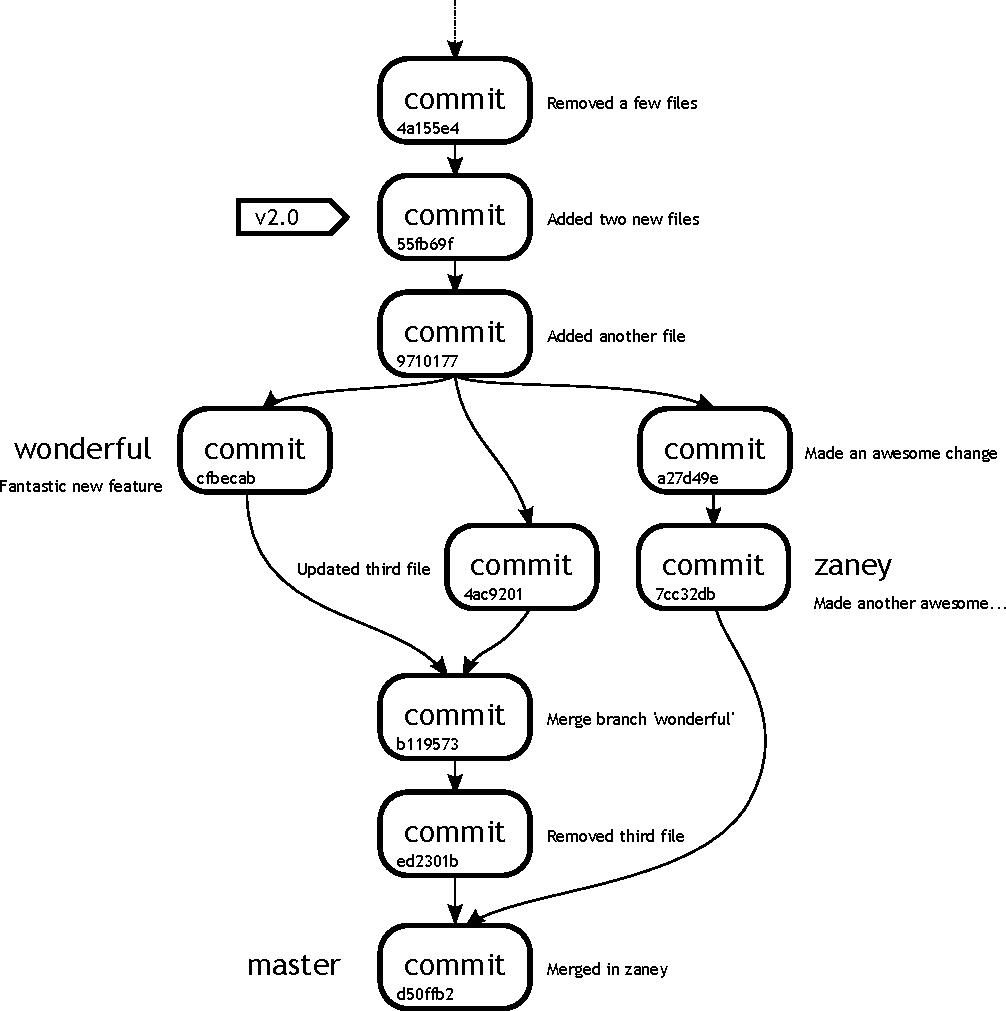
\includegraphics[width=9cm]{images/f-w4-d6.pdf}
\caption{Repository at the end of \emph{Week 4}}
\end{figure}

For arguments sake, let us say that we were on the \textbf{wonderful} branch, and we wanted to merge the \textbf{zaney} branch into it.
Using a standard 3-way merge algorithm, this would mean taking our current branch, which we will call \textbf{A}, the \textbf{zaney} branch, which we will call \textbf{B} and a parent which we will \textbf{C}.
Why do we need this parent? What is it used for?

\index{Best Common Ancestor}In order to merge changes from a specific file together, we need to know exactly how that file has changed over time.
In order to know that, we need to have a common starting point.
By that we mean that we need to have a state in both of the branches history, where \textbf{A} and \textbf{B} were the same.
In a version control system, this is most easily achieved by finding a commit that is common to the history of both branches.
This commit is called the \emph{Best Common Ancestor}.

Usually, when developing software, the code tree will be branched at various points along the way.
Sometimes we may need to merge these branches together, or merge these branches back into the master branch.
Which ever way we do it, we will need to find a common ancestor.
Figure 2, demonstrates a couple of possible merge proposals, and one of their common ancestors.

\begin{figure}[hbt]
\centering
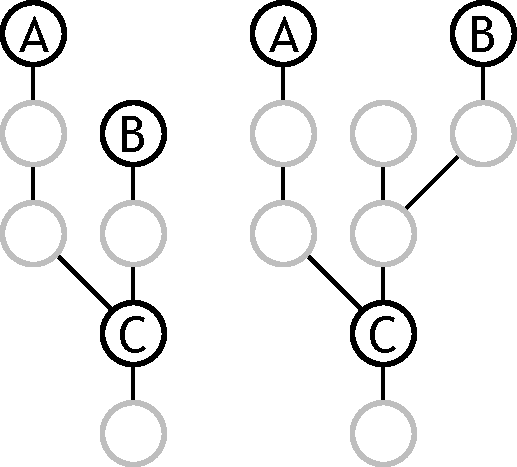
\includegraphics[width=6cm]{images/f-af4-d2.pdf}
\caption{Finding the \emph{Best Common Ancestor}}
\end{figure}

\index{Common Ancestor}As you can see from the second example, branch \textbf{B} was created from a commit above the \emph{Common Ancestor}, but the \emph{Common Ancestor} remains the same.

Let us go back to our example above.
We are attempting to merge in \textbf{zaney} to the \textbf{wonderful} branch.
We need to find the \textbf{C} in our equation.
To do this we could pour over Figure 1.
This should yield the result to be commit \textbf{9710177}.
Is there are way we can ask Git to do the same thing? The following output introduces a new command that is used to find the \emph{Best Common Ancestor} for a given merge proposal.

\begin{Verbatim}
john@satsuki:~/coderepo-af4$ git merge-base wonderful zaney
9710177657ae00665ca8f8027b17314346a5b1c4
john@satsuki:~/coderepo-af4$ git cat-file -p 9710177
tree 268f487e5c29a4b01c3a91637bac0024253fb77e
parent 55fb69f4ad26fdb6b90ac6f43431be40779962dd
author John Haskins <john.haskins@tamagoyakiinc.koala> 1301613377 +0100
committer John Haskins <john.haskins@tamagoyakiinc.koala> 1301613377
 +0100

Added another file
john@satsuki:~/coderepo-af4$
\end{Verbatim}

In our example, \indexgit{merge-base} uses two parameters to speficy the two heads that we wish to merge.
We can see that the commit that Git suggests as the \emph{Best Common Ancestor} is what we suggested above, \textbf{9710177}.
We have reused our \texttt{git cat-file} command to prove that the commit is the one we suggested, as you can see, the commit messages match.

This explains how a simple merge takes place, Git will find the common ancestor, and try to merge in the differences to produce a merged version.
If the merge cannot take place, then as shown in \emph{Week 4}, Git will put all the changes in the file, label them, and then raise a conflict for the user to resolve.

With the information presented here, you should now be able to reread the descriptions above and understand what is going on at a base level.
If you require further information on merging, there is a wealth of documentation and papers about merge algorithms on the Internet.

%reflog head

% chap5.tex - Week 5
\cleardoublepage
%\phantomsection
\chapter{Week 5}

\section{Day 1 - ``Conflicting information''}
\subsection{What to do when it all goes wrong}

The team have been playing with branches for a few days now and are beginning to settle into the idea of branching often.  As you can see, in Git, a branch is a really simple device for allowing experimentation and development.  As the implementation of branches is so simple, it is also really fast to switch between branches.  If you have been keeping up with the \emph{After Hours} sections, you can hopefully see that when switching branches, Git only needs to alter what is different between one working copy and another.

Let us see what new issues the team runs into during Week 5.

\begin{trenches}
``Hmm,'' the puzzled noise reverberated round Klaus' corner of the office.  Mumbling commenced.  ``So if I did that, then why is that not \ldots I mean I didn't think \ldots that's probably the problem Klaus \ldots sill 'luser'.''  He chuckled to himself, hardly noticing the looming figure of John.

``You got a conflict,'' said John matter of factly.

``I can see that,'' came Klaus' reply.  ``The problem is how do I solve it''

``What were you doing?''

``Well I had a few branches I had been working on and I was trying to merge them in.''

``Figures,'' said John.  
\end{trenches}

Conflicts are bound to happen at some point.  Even the best project processes in the world will sometimes end up with a conflict that has to be resolved.  We should, at this point, clarify what a conflict actually is.  A conflict occurs when an attempt is made to reconcile multiple changes to the same section of a file at the same time.  This usually means that the same line of code is modified by two different parties at the same time.  Now that we have several branches in our test repository, let us merge them back into master and see if we come up with a conflict.



%THIS IS TOO CONFUSING - NEED TO SIMPLIFY

\begin{Verbatim}[frame=leftline,framerule=1mm,fontsize=\relsize{-3}] 
john@akira:~/coderepo2$ git status
# On branch master
# Untracked files:
#   (use "git add <file>..." to include in what will be committed)
#
#	temp_file
nothing added to commit but untracked files present (use "git add" to track)
john@akira:~/coderepo2$ git merge wonderful 
Merge made by recursive.
 newfile1 |    1 +
 newfile2 |    1 +
 2 files changed, 2 insertions(+), 0 deletions(-)
john@akira:~/coderepo2$ git merge zaney 
Auto-merging newfile1
CONFLICT (content): Merge conflict in newfile1
Auto-merging newfile2
CONFLICT (content): Merge conflict in newfile2
Automatic merge failed; fix conflicts and then commit the result.
john@akira:~/coderepo2$ cat newfile1
A new file
<<<<<<< HEAD
and some more changes
=======
and some awesome changes
>>>>>>> zaney
john@akira:~/coderepo2$ cat newfile2
Another new file
<<<<<<< HEAD
and a new feature
=======
and some more awesome changes
>>>>>>> zaney
john@akira:~/coderepo2$ ls
another_file  my_third_committed_file  newfile1  newfile2  temp_file
john@akira:~/coderepo2$ nano newfile1

Error reading /home/john/.nano_history: Permission denied

Press Enter to continue starting nano.

john@akira:~/coderepo2$ cat newfile1 
A new file
and some more awesome changes
john@akira:~/coderepo2$ nano newfile2

Error reading /home/john/.nano_history: Permission denied

Press Enter to continue starting nano.

john@akira:~/coderepo2$ git status
# On branch master
# Unmerged paths:
#   (use "git add/rm <file>..." as appropriate to mark resolution)
#
#	both modified:      newfile1
#	both modified:      newfile2
#
# Untracked files:
#   (use "git add <file>..." to include in what will be committed)
#
#	temp_file
no changes added to commit (use "git add" and/or "git commit -a")
john@akira:~/coderepo2$ git add newfile1
john@akira:~/coderepo2$ git add newfile2
john@akira:~/coderepo2$ git status
# On branch master
# Changes to be committed:
#
#	modified:   newfile1
#	modified:   newfile2
#
# Untracked files:
#   (use "git add <file>..." to include in what will be committed)
#
#	temp_file
john@akira:~/coderepo2$ git commit -m 'Fixed conflicts in zaney merge'
[master a553c44] Fixed conflicts in zaney merge
john@akira:~/coderepo2$ !git log
git commit -m 'Fixed conflicts in zaney merge' log
error: pathspec 'log' did not match any file(s) known to git.
john@akira:~/coderepo2$ git log --graph --pretty=oneline --all --abbrev-commit --decorate
*   a553c44 (HEAD, master) Fixed conflicts in zaney merge
|\  
| * 4fdfe36 (zaney) Made another awesome change
| * 46c2390 Made an awesome change
* |   1db26b3 Merge branch 'wonderful'
|\ \  
| * | f0cbf32 (wonderful) Fantastic new feature
| |/  
* | 725c961 Continued Development
* | 6ab599d Important Update
|/  
* f91f31e Added another file
* 8d5140a (v2.0) Added two new files
* b5c84a5 Removed a few files
* fa65f06 (v1.0a) Messed with a few files
* 6ca160c Finished adding initial files
* e86ddea (v0.9) Made a few changes to first and second files
* 8820692 My First Ever Commit
john@akira:~/coderepo2$ gitk --all
^C
john@akira:~/coderepo2$ 
\end{Verbatim}

\section{Day 1 - ``No backup?''}
\subsection{Attack of the clones}

We now know about basic branching and merging.  At this stage, there is on important topic we must cover briefly, and this is subject of cloning.  Cloning allows you to make a complete copy of your repository, including all of its history and all of the branches.  Let us take a look at a situation which could make use of cloning.

\begin{trenches}
``So John,'' started Rob, ``Just how are we backing up the repository at the moment?''

John thought for a moment before replying.  He knew what Rob was getting at, but he hadn't expected Rob to bring the question up in front of Markus.  In truth he had forgotten all about it.  He turned to Markus.

``I'll be honest Markus.  Currently the repository isn't being backed up, but then we are running in parallel with the old system, so it would be the end of the world if we lost it.''

Markus nodded and smiled.  It seemed that John had gotten away with it for now and with that, Klaus shot Rob a piercing glance.  

``Team,'' began Markus, ``we need a definitive way of backing up the new Git repository, and I'd like it done before the end of the day.''  He pointed at a document on the table.  ``This project document has been approved by Wayne, and in there it states we will have a defined backup strategy.  Please don't let me down.''

\begin{center} * * * \end{center}

``Rob you really got to be careful about things like that,'' Klaus said to one of the younger members of the team.  ``You really showed John up in there.''  

``Yeh,'' said Rob, ``I realise that now.''  He stood with his back against the wall and tapped his fingers against the painted surface.  ``I was wondering, do you think John would let me look at the backup system for him as a way of apologising.''

Klaus smiled, it seemed Rob was finally understanding things, ``Go ask him,'' said Klaus, ``He's so snowed under with the BurnForce release that he'll probably let you implement it too''

``Right'' nodded Rob and off he went.
\end{trenches}

So cloning is an excellent way of taking a copy of our repository, in essence it is a simple way of taking a backup of our repository and keeping it up to date.  Obviously we could just take the files and copy them, but a better way of doing this is by utilising the \texttt{git clone} command.  When cloning a repository, we take then entire structure and replicate it, creating an exact copy of the data in an alternative location.  Well, that's what cloning means isn't it?

The git clone tool doesn't just copy the data though, it does several other things.  Let us create a clone of our test repository to another local location.  In this case, we are going to clone the repository into a folder called \texttt{coderepo-clone}.

\begin{Verbatim}[frame=leftline,framerule=1mm,fontsize=\relsize{-3}] 
john@akira:~$ git clone coderepo coderepo-clone
Initialized empty Git repository in /home/john/coderepo-clone/.git/
john@akira:~$ 
\end{Verbatim}

\begin{Verbatim}[frame=leftline,framerule=1mm,fontsize=\relsize{-3}] 
john@akira:~$ cd coderepo-clone
john@akira:~/coderepo-clone$ ls
another_file  my_third_committed_file  newfile1  newfile2
john@akira:~/coderepo-clone$
\end{Verbatim}

\begin{Verbatim}[frame=leftline,framerule=1mm,fontsize=\relsize{-3}] 
john@akira:~/coderepo-clone$ git status
# On branch master
nothing to commit (working directory clean)
john@akira:~/coderepo-clone$ 
\end{Verbatim}

Let us take a few moments to see what has happened here.  It would appear that our data has been copied successfully.  If you were to run a \texttt{git log} on this dir, you would see all the previous log messages for all our previous commits.  You can also see that if we run \texttt{git status} that we are on the same branch here that we were in our repository when we left it.  In this case, we are in the \textbf{master} branch.

\begin{trenches}
``Klaus, this doesn't make sense though.  I cloned my repo, but my branches have vanished,'' started Rob, rather worriedly.

``I'm sure they haven't gone anywhere,'' shouted John.  

Rob's reply was quick and certain, ``They have!  Run a git branch on your clone and see for yourself''

``Oh!''

Rob smiled the smug smile of a man who is pleased he was right.

\begin{center} * * * \end{center}

``Rob?'' asked John tentatively, aware of his previous state of anguish.

His reply indicated a less than stressed demeanour, ``Sup, dude?''.

John was pleasantly suprised, ``Did you sort out the branch issue?''

Rob begain walking over to John, ``Yeh, try running git branch with the r parameter.''

\end{trenches}

You may be thinking that we now have a detached copy of everything in our repository.  That's not exactly accurate.  Let us run the command that Rob suggested and see what is happening.  

\begin{Verbatim}[frame=leftline,framerule=1mm,fontsize=\relsize{-3}] 
john@akira:~/coderepo-clone$ git branch
* master
john@akira:~/coderepo-clone$ git branch -r
  origin/HEAD -> origin/master
  origin/master
  origin/wacky
john@akira:~/coderepo-clone$ 
\end{Verbatim}

Whilst we have all the objects in our repository, we do not yet have our branches set up locally.  They are available, but they have not been setup.  To explain this we need to introduce the concept of remote tracking branches.  We are familiar with local branches.  Local branches allowed us to make commits locally in a safe and separated environment.  Remote tracking branches are links to remote branches which allow us to track the development of that branch and bring it in to a local one if we so desire.

With a remote tracking branch, we can pull in the changes from the remote repository

Now we have a complete copy of our repository in another location.  At the moment we have created this clone on the same machine that our original is.  This isn't really a very good idea for backup purposes.  Git supplies several means with which to talk to a remote machine, but by far the most common of these is to utilise the SSH protocol.  SSH is a secure, encrypted way to communicate with a remote repository.  

If we assume that for a moment that our user john has now moved to another machine

In the next step, we are assuming that we have another machine where our user john has SSH access, and we are going to clone our repository there.

%POSSIBLY Talk about the SHARED and REFERENCE in a breakout
%POSSIBLY TALK ABOUT SSH
%ssh://[user@]host.xz[:port]/path/to/repo.git/




%branches
%merge
%remote tracking
%Itt section about not having anything backed up

%Parallel devving - ie...use both git and old for a while

% git show v1.0.0^{tree}

% afterhours5.tex - Afer Hours Week 5
\chapter{After Hours Week 5}
\section{``Splitting up commits the easy way''}
\subsection{Taking commits that little bit further}
Sometimes, putting everything in a single commit just is not a good idea.
Imagine you have pulled in number of updates to your working directory.
You may want to split these up.
It is true that you could simply \texttt{git add} only the files you want to include in the commit.
However, what happens when you have change four or five different things in the same file, and you want to split that commit up into five different commits.

There are two ways you can approach this.
The first is to copy the file in question out of the working directory, reset the working copy back to the last committed and copy your changes in line by line.
This can be time consuming and frustrating and when you are working on many files, it can be totally impractical.
What we need is a way to include or exclude certain lines of a file.

To demonstrate this we are going to create a new branch called \textbf{fantasy} and we are going to make several changes to a few files.
We are then going to show how the same process can be achieved by using both the GUI and the command line.

So let us start by creating our branch and making some changes as shown below.

\begin{code}
john@satsuki:~/coderepo$ git checkout -b fantasy
Switched to a new branch 'fantasy'
john@satsuki:~/coderepo$ echo "This is line 1" > newfile1
john@satsuki:~/coderepo$ echo "This is line 2" >> newfile1
john@satsuki:~/coderepo$ echo "This is line 3" >> newfile1
john@satsuki:~/coderepo$ echo "This is line 4" >> newfile1
john@satsuki:~/coderepo$ echo "This is a new line" >> newfile2
john@satsuki:~/coderepo$ echo "This is another new line" >> newfile2
\end{code}

Let us now just run a \texttt{git diff} to see exactly what the changes are.

\begin{code}
john@satsuki:~/coderepo$ git diff
diff --git a/newfile1 b/newfile1
index 44640b2..0eccf1a 100644
--- a/newfile1
+++ b/newfile1
@@ -1,2 +1,4 @@
-A new file
-and some more awesome changes
+This is line 1
+This is line 2
+This is line 3
+This is line 4
diff --git a/newfile2 b/newfile2
index 3545c1d..40efcce 100644
--- a/newfile2
+++ b/newfile2
@@ -1,2 +1,4 @@
 Another new file
 and a new awesome feature
+This is a new line
+This is another new line
john@satsuki:~/coderepo$
\end{code}

\index{hunk editing (cli)}Now, we could just do \texttt{git commit -a} and be done with it, but what if we really wanted to split this information up into four commits? We will introduce a new parameter to our \texttt{git add} tool from before.
We are going to use the \texttt{git add -p} or \texttt{git add --patch}.
This will allow us to interactively edit the hunks before they are committed.
To begin with, let us run \texttt{git add -p} and see what it is we need to do.

\begin{code}
john@satsuki:~/coderepo$ git add -p
diff --git a/newfile1 b/newfile1
index 44640b2..0eccf1a 100644
--- a/newfile1
+++ b/newfile1
@@ -1,2 +1,4 @@
-A new file
-and some more awesome changes
+This is line 1
+This is line 2
+This is line 3
+This is line 4
Stage this hunk [y,n,q,a,d,/,e,?]?
\end{code}

We are given the options of \texttt{y,n,q,a,d,/,e,?}.
At first glance, this may seem rather daunting.
Let us choose the \texttt{?} and see what help is presented to us.

\begin{code}
Stage this hunk [y,n,q,a,d,/,e,?]? ?
y - stage this hunk
n - do not stage this hunk
q - quit, do not stage this hunk nor any of the remaining ones
a - stage this and all the remaining hunks in the file
d - do not stage this hunk nor any of the remaining hunks in the file
g - select a hunk to go to
/ - search for a hunk matching the given regex
j - leave this hunk undecided, see next undecided hunk
J - leave this hunk undecided, see next hunk
k - leave this hunk undecided, see previous undecided hunk
K - leave this hunk undecided, see previous hunk
s - split the current hunk into smaller hunks
e - manually edit the current hunk
? - print help
@@ -1,2 +1,4 @@
-A new file
-and some more awesome changes
+This is line 1
+This is line 2
+This is line 3
+This is line 4
Stage this hunk [y,n,q,a,d,/,e,?]?
\end{code}

So it appears that Git is offering us the opportunity to either
\begin{itemize}
\item Stage it
\item Do not stage it
\item Quit,
\item Stage it and all remaining hunks
\item Do not stage it or any of the remaining ones
\item Search for a regex
\item Edit the hunk
\end{itemize}

In fact, though the help mentioned a \textbf{split} command, we do not have this option available to us, due to the nature of our hunk.
Instead, if we wish to split this hunk, we are going to have to edit it manually.
To do this we will choose the \texttt{e} option.

Here we are left in our chosen text editor, to either add, modify or remove lines from the hunk.
In our case, we are going to delete a few lines.
We only want to leave the first line of additions.
Just because we delete the others does not mean they are deleted from the working copy.
Remember, we are not editing the actual files here.
Just the hunks that are going to be staged.

\begin{code}
# Manual hunk edit mode -- see bottom for a quick guide
@@ -1,2 +1,4 @@
-A new file
-and some more awesome changes
+This is line 1
+This is line 2
+This is line 3
+This is line 4
# ---
# To remove '-' lines, make them ' ' lines (context).
# To remove '+' lines, delete them.
# Lines starting with # will be removed.
#
# If the patch applies cleanly, the edited hunk will immediately be
# marked for staging. If it does not apply cleanly, you will be given
# an opportunity to edit again. If all lines of the hunk are removed,
# then the edit is aborted and the hunk is left unchanged.
\end{code}

After the deletes, the editors file should look like this.

\begin{code}
# Manual hunk edit mode -- see bottom for a quick guide
@@ -1,2 +1,4 @@
-A new file
-and some more awesome changes
+This is line 1
# ---
# To remove '-' lines, make them ' ' lines (context).
# To remove '+' lines, delete them.
# Lines starting with # will be removed.
#
# If the patch applies cleanly, the edited hunk will immediately be
# marked for staging. If it does not apply cleanly, you will be given
# an opportunity to edit again. If all lines of the hunk are removed,
# then the edit is aborted and the hunk is left unchanged.
\end{code}

Once we quit our editor, we are then asked about the next hunk.
In our case, we are going to apply all of the changes to our second file during this commit.
To do this we are going to use the \texttt{a} option.

\begin{code}
diff --git a/newfile2 b/newfile2
index 3545c1d..40efcce 100644
--- a/newfile2
+++ b/newfile2
@@ -1,2 +1,4 @@
 Another new file
 and a new awesome feature
+This is a new line
+This is another new line
Stage this hunk [y,n,q,a,d,/,e,?]? a

john@satsuki:~/coderepo$
\end{code}

At first glance, we do not appear to have been left with any indication that anything has taken place.
In order to perform a check we shall run our obligatory \texttt{git diff}, both between the working copy and the index, and between the index and the last commit.

\begin{code}
john@satsuki:~/coderepo$ git diff
diff --git a/newfile1 b/newfile1
index f702b65..0eccf1a 100644
--- a/newfile1
+++ b/newfile1
@@ -1 +1,4 @@
 This is line 1
+This is line 2
+This is line 3
+This is line 4
john@satsuki:~/coderepo$
\end{code}

So above, we can see that the difference between the working copy and the index, or staging area, is the last three lines that we are not ready to commit yet.
Below we can see the difference between the staging area and the last commit to the repository.
This includes the three lines that we included during our interactive commit preparation.

\begin{code}
john@satsuki:~/coderepo$ git diff --cached
diff --git a/newfile1 b/newfile1
index 44640b2..f702b65 100644
--- a/newfile1
+++ b/newfile1
@@ -1,2 +1 @@
-A new file
-and some more awesome changes
+This is line 1
diff --git a/newfile2 b/newfile2
index 3545c1d..40efcce 100644
--- a/newfile2
+++ b/newfile2
@@ -1,2 +1,4 @@
 Another new file
 and a new awesome feature
+This is a new line
+This is another new line
john@satsuki:~/coderepo$
\end{code}

We can now commit in the normal way, and continue to edit the working copy to stage the sections we require.
The following output is shortened for brevity.

\begin{code}
john@satsuki:~/coderepo$ git commit -m 'Added first line'
[fantasy 03bd20c] Added first line
 2 files changed, 3 insertions(+), 2 deletions(-)
john@satsuki:~/coderepo$ git add -p
diff --git a/newfile1 b/newfile1
index f702b65..0eccf1a 100644
--- a/newfile1
+++ b/newfile1
@@ -1 +1,4 @@
 This is line 1
+This is line 2
+This is line 3
+This is line 4
Stage this hunk [y,n,q,a,d,/,e,?]? e

john@satsuki:~/coderepo$ git commit -m 'Added second line'
[fantasy 302e3fa] Added second line
 1 files changed, 1 insertions(+), 0 deletions(-)
john@satsuki:~/coderepo$ git add -p
...
...
\end{code}

We have gone through the process of editing each hunk for each commit and have performed the commits.

\begin{code}
john@satsuki:~/coderepo$ git log
commit a59e73b1dc571318a1154aa4c2fc591ab6f1f395
Author: John Haskins <john.haskins@tamagoyakiinc.koala>
Date:   Wed Apr 13 23:56:39 2011 +0100

    Added fourth line

commit 3ca3d627a54418be4c2e9d9196db6ce62e2b93ff
Author: John Haskins <john.haskins@tamagoyakiinc.koala>
Date:   Wed Apr 13 23:56:13 2011 +0100

    Added third line

commit 302e3fa5f880a2a503235667b4c96d4dcdaa11be
Author: John Haskins <john.haskins@tamagoyakiinc.koala>
Date:   Wed Apr 13 23:55:57 2011 +0100

    Added second line

commit 03bd20cb8a78a28f003ab402492cf7055f21bb2e
Author: John Haskins <john.haskins@tamagoyakiinc.koala>
Date:   Wed Apr 13 23:55:32 2011 +0100

    Added first line
...
...
\end{code}

\index{hunk editing(gui)}Next we are going to see how to perform exactly the same procedure using \texttt{git gui}.
For a start, we are going to reset our branch HEAD and our index back to their state before we made the last four commits, however we are going to leave the working copy files in the state they were after these last four commits.
This is called a \textbf{mixed} reset, as it modifies the staging area and the HEAD, but does not touch the working files.

\begin{code}
john@satsuki:~/coderepo$ git log --oneline
a59e73b Added fourth line
3ca3d62 Added third line
302e3fa Added second line
03bd20c Added first line
d50ffb2 Merged in zaney
ed2301b Removed third file
...
...
john@satsuki:~/coderepo$ git reset --mixed d50ffb2
Unstaged changes after reset:
M	newfile1
M	newfile2
john@satsuki:~/coderepo$
\end{code}

Now we will run a diff, just to be sure.

\begin{code}
john@satsuki:~/coderepo$ git diff
diff --git a/newfile1 b/newfile1
index 44640b2..0eccf1a 100644
--- a/newfile1
+++ b/newfile1
@@ -1,2 +1,4 @@
-A new file
-and some more awesome changes
+This is line 1
+This is line 2
+This is line 3
+This is line 4
diff --git a/newfile2 b/newfile2
index 3545c1d..40efcce 100644
--- a/newfile2
+++ b/newfile2
@@ -1,2 +1,4 @@
 Another new file
 and a new awesome feature
+This is a new line
+This is another new line
john@satsuki:~/coderepo$
\end{code}

If we now run our \texttt{git gui} command, we will see the changes that are present, once we click on one of the files in the left hand portion of the screen.
Let us start with \texttt{newfile2} as we want every change from that file present in this commit.
Figure 1 shows what \texttt{git gui} looks like at this stage.

\figuregith{10cm}{images/f-af5-d1.png}{Changes to \texttt{newfile2}}

If we right click on one of the green lines, remembering that green is short for an \textbf{addition}, we get a menu which we have not seen before.
Among other things, this menu has the ability to stage a specific line or hunk for commit.
In our case we are going to hit the \textbf{Stage Hunk For Commit} and then move on to the next file, \texttt{newfile1}.

\figuregith{10cm}{images/f-af5-d2.png}{Changes to \texttt{newfile1}}

Now we are looking at \texttt{newfile1}, we can use the \textbf{Stage Line For Commit} to add specific lines into the staging area.
The file is shown in Figure 2.
As our file is so small, we can run into problems if we just choose lines at random and stage them.
This is because it is hard for Git to find context around which to associate the change.
The context is the area immediately surrounding the change we are making.
In order to reduce the risk of the error occurring, we are simply going to start at the top, and select the first three lines for committing, by right clicking on each on in turn and choosing the \textbf{Stage Line For Commit} option from the menu.

We have the changes that we expect ready to be committed.
If we want to check one last time that they are right, we can use the \textbf{Staged Changes} pane on the left to choose the file and inspect the diff.
Once we are happy we can use the \textbf{Commit} area of the window to type our commit message and emblazon our changes forever.

\figuregith{10cm}{images/f-af5-d3.png}{Changes to \texttt{newfile1} after staging}

Figure 3, shows what our file looks like after the first commit.
Interestingly, as our file is so small, you will probably find that \texttt{git gui} throws a corrupt patch error if you try to just commit the next line.
As we mentioned earlier, it is always a good idea to know how to use the command line tools for precisely this reason.
Often you are dealing with special cases, that the GUI just can not handle.
In these cases, you may find you need to switch to the command line interface, to get the job done.

Let us now move back to our \textbf{master} branch and remove the \textbf{fantasy} branch.

\begin{code}
john@satsuki:~/coderepo$ git checkout master
Switched to branch 'master'
john@satsuki:~/coderepo$ git branch -D fantasy
Deleted branch fantasy (was 29ceede).
john@satsuki:~/coderepo$
\end{code}

Notice that because we used the capital \texttt{-D} parameter, we were not asked if we were sure we wanted to delete the \textbf{fantasy} branch.

So in the \emph{After Hours} section this week, we have found two ways to do the same complex task, one graphical and one command based.
Staging commits in this way may seem rather odd, but it will help you to keep your commits exceedingly exact.
Whilst this may not matter on a personal project, for Tamagoyaki Inc, grouping the right lines together in a commit will be an extremely useful process to have available.

% chap6.tex - Week 6
\cleardoublepage
%\phantomsection
\chapter{Week 6}

\section{Day 1 - ``My private little stash''}
\subsection{Getting interrrupted}

\index{stashing}We're getting close to the point where we can really start using Git as we originally intended, the team at Tamagoyaki Inc. are also getting much more acquainted with the operations of both version control and Git in particular.  Unfortunately things don't always go as smoothly as we would like.  The following scenario demonstrates just this.

\begin{trenches}
``Yeh but Martha, I need you to work on this fix now!  Not in five minutes.''

``Klaus I'm kinda in the middle of something else yet, and I'm not ready to commit,'' said Martha, feeling a little concerned.  She was used to Klaus making demands on his time, but she had spent a while working on this particular fix for John and she just wasn't ready to finish up yet.

``You could always use the stash feature.''  It was Rob again, it seemed as if this young user had cottoned on to Git quicker than most of the seasoned developers.''

Klaus seemed unimpressed, ``What the heck does that do?''

``Allows you to move your changes to somewhere else until you are ready to finish them.''

``Please Rob,'' started Martha, ``Can you show me what you mean?  Sounds exactly like what I need''
\end{trenches}

Sometimes you could be in the middle of something when another really important task comes up.  When this happens you are often required to drop everything and carry on with another task.  Often this can be quite difficult.  You may be in a development branch, but unable or unwilling to make a commit at this stage.  So how can we deal with this?

Well, one way of dealing with this situation, and this is not necessarily the best way, is to do the steps outlined below;

\begin{enumerate}
\item Make a new branch called something like WIP
\item Pull changes into this new branch
\item Commit changes into WIP branch
\item Switch back to the branch we need to work on
\item Make our changes and commit them
\item Merge in our WIP branch on top with the \texttt{--no-commit} option
\item Delete the WIP branch
\item Continue development in our original branch
\end{enumerate}

That may seem like a lot of work.  OK, the benefit is a fairly awesome one, but at the cost of considerable command line hackery to get there.  It would be nice if there was an easy way to do the above, and though someone of you may be screaming something like \emph{shell script} right about now, you can rest your fingers.  We actually have another tool in the Git toolbox to help us out.

The \indexgit{stash} command is used for exactly these situations.  Let us make a quick example of how to use it in our test repository.  To begin with we are going to make a few changes to the \textbf{master} branch, before we are interrupted.

\begin{Verbatim}
john@satsuki:~/coderepo$ git checkout master
Already on 'master'
john@satsuki:~/coderepo$ echo "Number strings rule 1234" >> 
 another_file
john@satsuki:~/coderepo$ 
\end{Verbatim}

\index{stashing!adding}So now we are interrupted and we have to make some important, and urgent changes to our \textbf{master} branch.  The example that follows is one way that we could use the \texttt{git stash} command to help us out.  

\begin{Verbatim}
john@satsuki:~/coderepo$ git stash
Saved working directory and index state WIP on master: d50ffb2 Merged 
 in zaney
HEAD is now at d50ffb2 Merged in zaney
john@satsuki:~/coderepo$ echo "Some mega important changes" >> newfile1
john@satsuki:~/coderepo$ git commit -a -m 'Important Update'
[master 9cb2af2] Important Update
 1 files changed, 1 insertions(+), 0 deletions(-)
john@satsuki:~/coderepo$ 
\end{Verbatim}

So using the \texttt{git stash} command, we have squirrelled all of our developmental changes away into a \emph{stash}.  Now we have completed the mega important change that just could not wait, we are ready to pull our changes back from the stash.  First let us see just what the stash contains.

\begin{Verbatim}
john@satsuki:~/coderepo$ git stash list
stash@{0}: WIP on master: d50ffb2 Merged in zaney
john@satsuki:~/coderepo$ git stash show stash@{0}
 another_file |    1 +
 1 files changed, 1 insertions(+), 0 deletions(-)
john@satsuki:~/coderepo$ git stash show stash@{0} -p
diff --git a/another_file b/another_file
index dba885d..b3a5cc5 100644
--- a/another_file
+++ b/another_file
@@ -1 +1,2 @@
 New stuff
+Number strings rule 1234
john@satsuki:~/coderepo$ 
\end{Verbatim}

\index{stashing!showing}As you can see, the \texttt{-p} option to the \texttt{git stash show} command shows us exactly what is contained in the stash.  We can apply this stash by running the following;

\begin{Verbatim}
john@satsuki:~/coderepo$ git stash apply stash@{0}
# On branch master
# Changed but not updated:
#   (use "git add <file>..." to update what will be committed)
#   (use "git checkout -- <file>..." to discard changes in working 
 directory)
#
#	modified:   another_file
#
# Untracked files:
#   (use "git add <file>..." to include in what will be committed)
#
#	my_third_committed_file
#	temp_file
no changes added to commit (use "git add" and/or "git commit -a")
john@satsuki:~/coderepo$ git commit -a -m 'Continued Development'
[master 37950f8] Continued Development
 1 files changed, 1 insertions(+), 0 deletions(-)
john@satsuki:~/coderepo$ git stash list
stash@{0}: WIP on master: d50ffb2 Merged in zaney
john@satsuki:~/coderepo$ 
\end{Verbatim}

Our stash has been applied to the current branch, in our case \textbf{master}, and we have gone ahead and committed these changes into the repository.  In this case we didn't have anything else to add to the index before we went ahead and committed it.  

\index{stashing!removing}Interestingly though, our stash still exists.  If we had used the \texttt{git stash pop} command instead of the \texttt{git stash apply}, our stash would have been removed.  Of course we can have multiple stashes in our repository.  For completeness sake, let us learn how to manually remove a stash, and take a look at how our repository looks with our semi-graphical \texttt{git log}

\begin{Verbatim}
john@satsuki:~/coderepo$ git stash drop stash@{0}
Dropped stash@{0} (193f27172fc0df278105b981815c7718204030d8)
john@satsuki:~/coderepo$ git log --graph --pretty=oneline --all 
 --abbrev-commit --decorate
* 37950f8 (HEAD, master) Continued Development
* 9cb2af2 Important Update
*   d50ffb2 Merged in zaney
|\  
| * 7cc32db (zaney) Made another awesome change
| * a27d49e Made an awesome change
* | ed2301b Removed third file
* |   b119573 Merge branch 'wonderful'
|\ \  
| * | cfbecab (wonderful) Fantastic new feature
| |/  
* | 4ac9201 Updated third file
|/  
* 9710177 Added another file
* 55fb69f (v2.0) Added two new files
* 4a155e4 Removed a few files
* a022d4d (tag: v1.0b, v1.0a) Messed with a few files
* 9938a0c Finished adding initial files
* 163f061 (v0.9) Made a few changes to first and second files
* cfe23cb My First Ever Commit
john@satsuki:~/coderepo$ 
\end{Verbatim}

So using the \texttt{git stash drop} command, you can see that it is fairly simple to drop a single stash from the list.


\section{Day 2 - ``What?! No backup?''}
\subsection{Attack of the clones}

We now know about basic branching and merging.  At this stage, there is on important topic we must cover briefly, and this is subject of cloning.  Cloning allows you to make a complete copy of your repository, including all of its history and all of the branches.  Let us take a look at a situation which could make use of cloning.

\begin{trenches}
``So John,'' started Rob, ``Just how are we backing up the repository at the moment?''

John thought for a moment before replying.  He knew what Rob was getting at, but he hadn't expected Rob to bring the question up in front of Markus.  In truth he had forgotten all about it.  He turned to Markus.

``I'll be honest Markus.  Currently the repository isn't being backed up, but then we are running in parallel with the old system, so it wouldn't be the end of the world if we lost it.''

Markus nodded and smiled.  It seemed that John had gotten away with it for now and with that, Klaus shot Rob a piercing glance.  

``Team,'' began Markus, ``we need a definitive way of backing up the new Git repository, and I'd like it done before the end of the day.''  He pointed at a document on the table.  ``This project document has been approved by Wayne, and in there it states we will have a defined backup strategy.  Please don't let me down.''

\thoughtbreak

``Rob you really got to be careful about things like that,'' Klaus said to one of the younger members of the team.  ``You really showed John up in there.''  

``Yeh,'' said Rob, ``I realise that now.''  He stood with his back against the wall and tapped his fingers against the painted surface.  ``I was wondering, do you think John would let me look at the backup system for him as a way of apologising.''

Klaus smiled, it seemed Rob was finally understanding things, ``Go ask him,'' said Klaus, ``He's so snowed under with the BurnForce release that he'll probably let you implement it too''

``Right'' nodded Rob and off he went.
\end{trenches}

\index{cloning}So cloning is an excellent way of taking a copy of our repository, in essence it is a simple way of taking a backup of our repository and then with a little more work, we can keep that clone up to date.  Obviously we could just take the files and copy them, but a better way of doing this is by utilising the \indexgit{clone} command.  When cloning a repository, we take then entire structure and replicate it, creating an exact copy of the data in an alternative location.  Well, that's what cloning means isn't it?

The git clone tool doesn't just copy the data though, it does several other things.  Let us create a clone of our test repository to another local location.  In this case, we are going to clone the repository into a folder called \texttt{coderepo-cl}.

\begin{Verbatim}
john@satsuki:~$ git clone coderepo coderepo-cl
Initialized empty Git repository in /home/john/coderepo-cl/.git/
john@satsuki:~$ 
\end{Verbatim}

\begin{Verbatim}
john@satsuki:~$ cd coderepo-cl
john@satsuki:~/coderepo-cl$ ls 
another_file  newfile1  newfile2
john@satsuki:~/coderepo-cl$
\end{Verbatim}

\begin{Verbatim}
john@satsuki:~/coderepo-cl$ git status
# On branch master
nothing to commit (working directory clean)
john@satsuki:~/coderepo-cl$ 
\end{Verbatim}

Let us take a few moments to see what has happened here.  It would appear that our data has been copied successfully.  If you were to run a \texttt{git log} on this dir, you would see all the previous log messages for all our previous commits.  You can also see that if we run \texttt{git status} that we are on the same branch here that we were in our repository when we left it.  In this case, we are in the \textbf{master} branch.

So this could be sufficient enough to serve as a backup of our repository, but we will actually find a better way to do this a little later.

\section{Day 3 - ``Is this clone for real?''}
\subsection{Not entirely as expected}

We now have a clone of the repository and we can start to look at how we can play with branches and see how the two are different.

\begin{trenches}
``Klaus, this doesn't make sense though.  I cloned my repo, but my branches have vanished,'' started Rob, rather worriedly.

``I'm sure they haven't gone anywhere,'' shouted John.  

Rob's reply was quick and certain, ``They have!  Run a git branch on your clone and see for yourself''

``Oh!''

Rob smiled the smug smile of a man who is pleased he was right.

\thoughtbreak

``Rob?'' asked John tentatively, aware of his previous state of anguish.

His reply indicated a less than stressed demeanour, ``Sup, dude?''.

John was pleasantly surprised, ``Did you sort out the branch issue?''

Rob began walking over to John, ``Yeh, try running git branch with the r parameter.''

\end{trenches}

\index{branching!remote}You may be thinking that we now have a detached copy of the other branches in our repository.  That's not exactly accurate.  Let us run the command that Rob suggested and see what is happening.  

\begin{Verbatim}
john@satsuki:~/coderepo-cl$ git branch
* master
john@satsuki:~/coderepo-cl$ git branch -r
  origin/HEAD -> origin/master
  origin/master
  origin/wonderful
  origin/zaney
john@satsuki:~/coderepo-cl$ 
\end{Verbatim}

Whilst we have all the objects in our repository, we do not yet have our branches set up locally.  They are available, but they have not yet been setup locally.  To explain this we need to introduce the concept of remote tracking branches.  We are familiar with local branches.  Local branches allowed us to make commits locally in a safe and separated environment.  Remote tracking branches are links to remote branches which allow us to track the development of that branch and bring it in to a local one if we so desire.

Let us take a look at what we can do with these remote tracking branches.  Notice in the output above, we have the word \texttt{origin} in front of the branch names.  When we clone a repository, Git automatically sets up what is called a \emph{remote}.  We can view this by using the \indexgit{remote} tool.

\begin{Verbatim}
john@satsuki:~/coderepo-cl$ git remote
origin
john@satsuki:~/coderepo-cl$ git remote -v
origin	/home/john/coderepo (fetch)
origin	/home/john/coderepo (push)
john@satsuki:~/coderepo-cl$ 
\end{Verbatim}

As you can see from the output above, the \textbf{origin} remote definition points to the original folder that our repository came from.  So now we know that when referring to \texttt{origin/master}, we are really talking about the \textbf{master} branch which is located at the remote location \textbf{origin}.

We are going to spend a little while now learning about remote branches and how they differ to local branches.  Let us spend a few minutes trying some of our normal operations against a remote branch.  The first operation we are going to try is a diff.  We are going to run a diff between our current \textbf{master} branch and the \textbf{wonderful} branch as it stands in the original repository, so we should be diffing between \texttt{master} and \texttt{origin/wonderful}.  For brevity, we are also going to limit the changes shown to those which affect \texttt{newfile1} only, by appending \texttt{ -- <filename>} to the command.

\begin{Verbatim}
john@satsuki:~/coderepo-cl$ git diff master origin/wonderful -- 
 newfile1
diff --git a/newfile1 b/newfile1
index f32a0e6..ef20984 100644
--- a/newfile1
+++ b/newfile1
@@ -1,3 +1,2 @@
 A new file
-and some more awesome changes
-Some mega important changes
+and some more changes
john@satsuki:~/coderepo-cl$ 
\end{Verbatim}

So we can see that our diff command completed successfully.  Note that this command requires no connection to our \textbf{origin} repository, as all of the data has been cloned locally, more on this later.  

Let us run another command now and learn a little more about what the remote reference \textbf{origin} really means.

\begin{Verbatim}
john@satsuki:~/coderepo-cl$ git remote show origin
* remote origin
  Fetch URL: /home/john/coderepo
  Push  URL: /home/john/coderepo
  HEAD branch: master
  Remote branches:
    master    tracked
    wonderful tracked
    zaney     tracked
  Local branch configured for 'git pull':
    master merges with remote master
  Local ref configured for 'git push':
    master pushes to master (up to date)
john@satsuki:~/coderepo-cl$ 
\end{Verbatim}

Though this command introduces some terms that we are not yet familiar with yet, like push, pull and fetch, we can see that the \textbf{origin} remote has been set up to \emph{track} three branches called, \textbf{master}, \textbf{wonderful} and \textbf{zaney}.  So although these branches are not yet usable in the way a local branch would be, it is comforting to know that Git does know about them.  Let us continue playing with the remote branch and run a \texttt{git log} command against it.

\begin{Verbatim}
john@satsuki:~/coderepo-cl$ git log origin/master -- newfile1
commit 9cb2af2a00fd2253060e6bf8cc6c377b3d55ecea
Author: John Haskins <john.haskins@tamagoyakiinc.koala>
Date:   Tue Apr 19 16:43:59 2011 +0100

    Important Update

commit d50ffb2fa536d869f2c4e89e8d6a48e0a29c5cc1
Merge: ed2301b 7cc32db
Author: John Haskins <john.haskins@tamagoyakiinc.koala>
Date:   Fri Apr 1 07:42:04 2011 +0100

    Merged in zaney

...
...
...
\end{Verbatim}

Again, this requires no connection to the \textbf{origin} repository at all and works as expected.  Let us try something really funky now, let us try checking out a remote branch so that we can view the filesystem.  We are now going to try checking out the remote branch called \textbf{wonderful}.

\begin{Verbatim}
john@satsuki:~/coderepo-cl$ git checkout origin/wonderful
Note: checking out 'origin/wonderful'.

You are in 'detached HEAD' state. You can look around, make 
experimental changes and commit them, and you can discard any 
commits you make in this state without impacting any branches 
by performing another checkout.

If you want to create a new branch to retain commits you create, you 
may do so (now or later) by using -b with the checkout command again. 
Example:

  git checkout -b new_branch_name

HEAD is now at cfbecab... Fantastic new feature
john@satsuki:~/coderepo-cl$ 
\end{Verbatim}

\index{dangling}Interesting.  This is not what we are used to seeing.  When we have checked out branches before, we have always been presented with a \texttt{Switched to branch 'xxxxxx'} message.  Now we are seeing a funny message about having a detatched HEAD.  This is because we are not actually on a branch.  We can make changes as we are advised, we can even make commits, but these will not actually become integrated into any branches.  In essence these commits would be left dangling and after time, because no branch points to them, they would get deleted by garbage collection routines.

Running the \texttt{git branch} command below confirms our suspicions.

\begin{Verbatim}
john@satsuki:~/coderepo-cl$ git branch -v
* (no branch) cfbecab Fantastic new feature
  master      37950f8 Continued Development
john@satsuki:~/coderepo-cl$ 
\end{Verbatim}

\index{branching!tracking}So we really need to figure out how to make these branches exist locally so that we can commit to them and retain those commits.  To do this we use the \texttt{git branch} tool again, but we use it in a slightly different manner.  

\begin{Verbatim}
john@satsuki:~/coderepo-cl$ git checkout -b wonderful origin/wonderful 
Branch wonderful set up to track remote branch wonderful from origin.
Switched to a new branch 'wonderful'
john@satsuki:~/coderepo-cl$ 
\end{Verbatim}

We are now on a local instance of the \textbf{wonderful} branch.  Let us take a minute to understand what that means.  As Git is a distributed environment, our local \textbf{wonderful} branch, is not going to be synchronised with the remote end automatically.  It would require effort on our part.  What this does mean though, is that we are able to begin committing to this branch and experimenting with it.

\section{Day 4 - ``Help I'm no longer up to date?''}
\subsection{Pulling changes, not teeth}

With a remote tracking branch, we can pull in the changes from the remote repository.  In our case, the remote repository is in the \texttt{coderepo} directory that we created at the start of the book.  In the \texttt{coderepo-cl} directory we have a separate, self-contained copy of the repository.  At the moment, because no changes have occurred to either, they contain exactly the same data.

By running the \texttt{git remote} tool again, we can see which branches are set up locally to track their remote counterparts in \textbf{origin}.

\begin{Verbatim}
john@satsuki:~/coderepo-cl$ git remote show origin
* remote origin
  Fetch URL: /home/john/coderepo
  Push  URL: /home/john/coderepo
  HEAD branch: master
  Remote branches:
    master    tracked
    wonderful tracked
    zaney     tracked
  Local branches configured for 'git pull':
    master    merges with remote master
    wonderful merges with remote wonderful
  Local refs configured for 'git push':
    master    pushes to master    (up to date)
    wonderful pushes to wonderful (up to date)
john@satsuki:~/coderepo-cl$ 
\end{Verbatim}

What we are going to do now is make some changes to our original repository and see how we can view those changes and indeed pull them into our current local working repository, or clone.  Note that in the following code examples we have switched back to working on our original repository, in the \texttt{coderepo} folder.

\begin{Verbatim}
john@satsuki:~/coderepo-cl$ cd ../coderepo
john@satsuki:~/coderepo$ git branch
* master
  wonderful
  zaney
john@satsuki:~/coderepo$ git checkout wonderful 
Switched to branch 'wonderful'
john@satsuki:~/coderepo$ git merge master
Updating cfbecab..37950f8
Fast-forward
 another_file            |    1 +
 my_third_committed_file |    1 -
 newfile1                |    3 ++-
 newfile2                |    2 +-
 4 files changed, 4 insertions(+), 3 deletions(-)
 delete mode 100644 my_third_committed_file
john@satsuki:~/coderepo$ echo "These changes are in the origin" >> 
 newfile3
john@satsuki:~/coderepo$ git add newfile3
john@satsuki:~/coderepo$ git commit -a -m 'Added a new file'
[wonderful 1c3206a] Added a new file
 1 files changed, 1 insertions(+), 0 deletions(-)
 create mode 100644 newfile3
john@satsuki:~/coderepo$ 
\end{Verbatim}

As you can see, we have switched back to working on our old \textbf{orgin} and have bought \textbf{wonderful} to be in line with master and have added a new file and committed the changes.  Now let us go back to our clone and see if we can see those changes.

\begin{Verbatim}
john@satsuki:~/coderepo$ cd ../coderepo-cl/
john@satsuki:~/coderepo-cl$ git diff wonderful origin/
origin/HEAD        origin/master      origin/wonderful   origin/zaney 
john@satsuki:~/coderepo-cl$ git diff wonderful origin/wonderful 
john@satsuki:~/coderepo-cl$ 
\end{Verbatim}

That seems a little odd at first glance.  We have tried to view a diff between our local \textbf{wonderful} branch and the remote \textbf{origin/wonderful} branch.  Interestingly, Git is telling us that there is no difference.  Hang on though, we just made some changes above.  

Remember before we discussed the fact that our clone was disconnected from the \textbf{origin} copy?  What this means is that unless we ask Git, it won't update details about what is present in the remote copy.  Once this is up to date, we can pull the changes into our local copy of the remote branch?  Interestingly there are actually two ways to do this.

\index{branching!updating remote}The first method is by running a \indexgit{pull} command.  If you remember the output from the \texttt{git remote show origin}, you may remember that it showed that there was a local branch configured for \texttt{'git pull'} and the details it gave for the \textbf{wonderful} branch were as follows; \texttt{wonderful merges with remote wonderful}.  What this means, is that when we run a \texttt{git pull} from inside the \textbf{wonderful} branch, Git will automatically contact the remote repository, update the list of changes and merge them into the local branch if possible.

We mentioned that there were two methods to perform the procedure.  Whilst the first one is to use \texttt{git pull}, the second one actually achieves an almost identical result, but by running two commands instead of one.  In point of fact, these two commands are executed by the \texttt{git pull} command.  Running them as two separate commands allows us to understand a little more about what is happening.  Let us run the command and then explain what we have done.

\begin{Verbatim}
john@satsuki:~/coderepo-cl$ git fetch origin
remote: Counting objects: 4, done.
remote: Compressing objects: 100% (2/2), done.
remote: Total 3 (delta 1), reused 0 (delta 0)
Unpacking objects: 100% (3/3), done.
From /home/john/coderepo
   cfbecab..1c3206a  wonderful  -> origin/wonderful
john@satsuki:~/coderepo-cl$ git diff wonderful origin/wonderful 
diff --git a/another_file b/another_file
index dba885d..b3a5cc5 100644
--- a/another_file
+++ b/another_file
@@ -1 +1,2 @@
 New stuff
+Number strings rule 1234
...
...
...

john@satsuki:~/coderepo-cl$ git merge origin/wonderful 
Updating cfbecab..1c3206a
Fast-forward
 another_file            |    1 +
 my_third_committed_file |    1 -
 newfile1                |    3 ++-
 newfile2                |    2 +-
 newfile3                |    1 +
 5 files changed, 5 insertions(+), 3 deletions(-)
 delete mode 100644 my_third_committed_file
 create mode 100644 newfile3
john@satsuki:~/coderepo-cl$ 
\end{Verbatim}

As you can see, the two commands that we used were \indexgit{fetch} and the more familiar \texttt{git merge}.  The \texttt{git fetch} command literally visits the remote repository, in our case we asked for \textbf{origin}, and finds which objects are new.  These are then copied to the local clone, and the HEADs of the various remote branches are updated.  We now rerun our \texttt{git diff}, only this time, we see a great many more changes than before.  Finally we initiate a \texttt{git merge} to pull the changes from the now up to date remote branch to our local one.

We could have used the \texttt{git pull} command here, and if we had supplied no parameters to it, it would have achieved the exact same outcome.  The only difference would have been running one command instead of two.  Please note, that there are occasions when you would require one over the other, but as an introduction, this should be sufficient.

\section{Day 5 - ``I'm putting my foot down''}
\subsection{Pushing back!}

We now know a lot about remote locations right?  We are ready to start collaborating with someone.  Let us first see how Tamagoyaki are getting on with things.

\begin{trenches}
``But I know I have the remote right Simon, it's giving some weird error about refusing to update it.''  Rob was getting more than a little cross now.  

``Maybe you got the command wrong?'' asked Simon.

Rob slammed his hands down on the keyboard, ``Well then you come over here and type it, but I don't understand how hard it is to write git push.''  He shook his head, ``I even checked using the git remote tool and the push is apparently all set up.''

``Are you trying to push to a non-bare repository?'' Chirped Klaus.  He had been listening to the discussion escalate from mild annoyance to key shattering intrusion.  ``You can't push to a non-bare repository, else everything gets out of sync.''

``What do you mean bare?'' asked Rob.

Klaus smiled and his head appeared over the cubicle.  ``Come over here genius and I'll show you,'' he said with the slightest amount of gloat at being one of the only people to know something about Git that Rob didn't.
\end{trenches}

\index{bare repository}\index{non-bare repository}\index{pushing}Bare?  Non-bare?  At first glance, this may seem confusing.  It isn't exactly an intuitive word to describe a repository but what Klaus mentioned was absolutely true.  In Git, if you want to push changes back to a repository, instead of pulling them, the repository that you push to should be what is called a \emph{bare} repository.  What this means is that the repository has no working copy.

\begin{callout}{Note}{Pushing to a non-bare repository}
As mentioned, pushing to a non-bare repository is not a good idea.  When you push to a repository, you update the objects in the objects database.  This will affect commits, blobs and trees.  We should make a distinction here.  We are really only worried about pushing to a branch which is currently checked out.  Pushing to a non-bare repository will mean that the index will get changed, as it should reflect what the branch looks like at HEAD.  
\newline
\newline
Now this causes a problem when we are trying to see what has been modified in the working directory when compared to the HEAD.  As our working copy will contain older versions of the files than are in the index, it will appear as if many more changes have occured and we risk undoing those changes.  For these reasons, it is much simpler just to push only to bare repositories.
\end{callout}

At first glance this may seem like a rather odd thing to want.  Why would we want a repository that doesn't have a working tree?  The simple answer is that a \emph{bare} repository allows us to be able to push changes into it.  Let us recreate the error message that Rob was talking about.

\begin{Verbatim}
john@satsuki:~/coderepo-cl$ echo "This is another update to newfile3" 
 >> newfile3
john@satsuki:~/coderepo-cl$ git commit -a -m 'Added more to newfile3'
[wonderful dbf1e9a] Added more to newfile3
 1 files changed, 1 insertions(+), 0 deletions(-)
\end{Verbatim}

We have made a modification to the \textbf{wonderful} branch.  So let us now try to push that back to the \textbf{origin} remote repository with the \indexgit{push} command.
 
\begin{Verbatim}
john@satsuki:~/coderepo-cl$ git push
Counting objects: 5, done.
Compressing objects: 100% (3/3), done.
Writing objects: 100% (3/3), 335 bytes, done.
Total 3 (delta 1), reused 0 (delta 0)
Unpacking objects: 100% (3/3), done.
remote: error: refusing to update checked out branch: 
 refs/heads/wonderful
remote: error: By default, updating the current branch in a non-bare 
remote: error: repository is denied, because it will make the index 
remote: error: and work tree inconsistent with what you pushed, and 
remote: error: will require 'git reset --hard' to match the work 
remote: error: tree to HEAD.
remote: error: 
remote: error: You can set 'receive.denyCurrentBranch' configuration 
remote: error: variable to 'ignore' or 'warn' in the remote repository 
remote: error: to allow pushing into its current branch; however, this 
remote: error: is not recommended unless you arranged to update its 
remote: error: work tree to match what you pushed in some other way.
remote: error: 
remote: error: To squelch this message and still keep the default 
remote: error: behaviour, set 'receive.denyCurrentBranch' configuration 
remote: error: variable to 'refuse'.
To /home/john/coderepo
 ! [remote rejected] wonderful -> wonderful (branch is currently checked out)
error: failed to push some refs to '/home/john/coderepo'
john@satsuki:~/coderepo-cl$ 
\end{Verbatim}

Bingo!  There is the error we were looking for.  In order to get round this, we are going to create another clone of the repository in \texttt{coderepo}.  This time however, we are going to pass an option to it when we create it.

\begin{Verbatim}
john@satsuki:~/coderepo-cl$ cd ..
john@satsuki:~$ git clone coderepo coderepo-bk --bare
Initialized empty Git repository in /home/john/coderepo-bk/
john@satsuki:~$ cd coderepo-bk/
john@satsuki:~/coderepo-bk$ ls
branches  config  description  HEAD  hooks  info  objects  
packed-refs  refs
john@satsuki:~/coderepo-bk$ cd ..
john@satsuki:~$ cd coderepo-cl/
john@satsuki:~/coderepo-cl$ 
\end{Verbatim}

As you can see, creating the clone with the \texttt{--bare} option has had a definite effect on the structure of the clone itself.  In fact, the contents of the \texttt{coderepo-bk} folder look remarkably similar to the \texttt{.git} folder found in our normal working tree.  They are in fact, one and the same.  We have removed the need for a separate \texttt{.git} folder because we do not require a working tree.  Therefore, the contents of the \texttt{.git} folder and placed in the root \texttt{coderepo-bk} folder.

\index{remote!adding}We are getting closer to making our push.  We have created a \emph{bare} repository, which we should now be able to push to.  The problem is, we have not yet defined our new repository as a remote location in the \texttt{coderepo-cl} repository.  This is something we will do now and to do this, we will use our \texttt{git remote} tool once more, this time employing the \texttt{add} parameter.

\begin{Verbatim}
john@satsuki:~/coderepo-cl$ git remote add backup 
 /home/john/coderepo-bk
john@satsuki:~/coderepo-cl$ git remote show backup
* remote backup
  Fetch URL: /home/john/coderepo-bk
  Push  URL: /home/john/coderepo-bk
  HEAD branch: wonderful
  Remote branches:
    master    new (next fetch will store in remotes/backup)
    wonderful new (next fetch will store in remotes/backup)
    zaney     new (next fetch will store in remotes/backup)
  Local refs configured for 'git push':
    master    pushes to master    (up to date)
    wonderful pushes to wonderful (fast-forwardable)
john@satsuki:~/coderepo-cl$ 
\end{Verbatim}

We have created a remote called backup.  As you can see, some interrogation of the remote repository has taken place.  It is already aware of the branches present in our remote location.  Let us do a \texttt{git fetch} to update the local references.

\begin{Verbatim}
john@satsuki:~/coderepo-cl$ git fetch backup
From /home/john/coderepo-bk
 * [new branch]      master     -> backup/master
 * [new branch]      wonderful  -> backup/wonderful
 * [new branch]      zaney      -> backup/zaney
john@satsuki:~/coderepo-cl$ git remote show backup
* remote backup
  Fetch URL: /home/john/coderepo-bk
  Push  URL: /home/john/coderepo-bk
  HEAD branch: wonderful
  Remote branches:
    master    tracked
    wonderful tracked
    zaney     tracked
  Local refs configured for 'git push':
    master    pushes to master    (up to date)
    wonderful pushes to wonderful (fast-forwardable)
john@satsuki:~/coderepo-cl$ 
\end{Verbatim}

Now we can see that all of the remote references for our \textbf{backup} remote have been updated.  If we run a diff against our local \textbf{wonderful} branch and the remote branch \textbf{backup/wonderful}, we can see the differences.

\begin{Verbatim}
john@satsuki:~/coderepo-cl$ git diff wonderful backup/wonderful 
diff --git a/newfile3 b/newfile3
index 7268b97..638113c 100644
--- a/newfile3
+++ b/newfile3
@@ -1,2 +1 @@
 These changes are in the origin
-This is another update to newfile3
john@satsuki:~/coderepo-cl$ git branch -v
\end{Verbatim}

There we go!  Those are the changes we just committed to the local repository.  The last thing we need to do is to initiate a \texttt{git push}.  We are going to have to define which remote we wish to push to now for two reasons.  The first is that now we have two remotes, and so Git would not know if we meant \textbf{origin} or \textbf{backup}.  The second reason is that by default, the \textbf{wonderful} branch is set up to push to the \textbf{origin} remote.

\begin{Verbatim}
john@satsuki:~/coderepo-cl$ git push backup
Counting objects: 5, done.
Compressing objects: 100% (3/3), done.
Writing objects: 100% (3/3), 335 bytes, done.
Total 3 (delta 1), reused 0 (delta 0)
Unpacking objects: 100% (3/3), done.
To /home/john/coderepo-bk
   1c3206a..dbf1e9a  wonderful -> wonderful
john@satsuki:~/coderepo-cl$ 
\end{Verbatim}

There we go, we have now managed to push our changes to a remote location.  In this case, we have pushed an update from the \textbf{wonderful} branch to the \textbf{backup/wonderful branch}.  If we wanted to, we could have pushed our repository to a new branch name, or indeed any of the existing branch names.

\begin{Verbatim}
john@satsuki:~/coderepo-cl$ git push backup wonderful:newbranch
Total 0 (delta 0), reused 0 (delta 0)
To /home/john/coderepo-bk
 * [new branch]      wonderful -> newbranch
john@satsuki:~/coderepo-cl$ git remote show backup
* remote backup
  Fetch URL: /home/john/coderepo-bk
  Push  URL: /home/john/coderepo-bk
  HEAD branch (remote HEAD is ambiguous, may be one of the following):
    newbranch
    wonderful
  Remote branches:
    master    tracked
    newbranch tracked
    wonderful tracked
    zaney     tracked
  Local refs configured for 'git push':
    master    pushes to master    (up to date)
    wonderful pushes to wonderful (up to date)
john@satsuki:~/coderepo-cl$ 
\end{Verbatim}

By specifying the local and remote branch using the \texttt{local:remote} syntax, we have told Git to push our local \textbf{wonderful} branch to the remote branch called \textbf{newbranch}.  As the \textbf{newbranch} did not exist in the remote \textbf{backup} repository, it was created, as can be seen above.

So this ends the Week.  We have learnt a lot more about how to play with branches and remotes.  In the \emph{After Hours} section, we will take a deeper look at remote branches and how they are configured and represented in Git.

DEFAULT GIT PULL

%POSSIBLY Talk about the SHARED and REFERENCE in a breakout
%POSSIBLY TALK ABOUT SSH
%ssh://[user@]host.xz[:port]/path/to/repo.git/

\clearpage

\section{Summary - John's Notes}
\subsection{Commands}
\begin{itemize}

\item\texttt{git stash} - Short for \texttt{git stash save}, creates a stash of local modifications

\item\texttt{git stash apply <stash\_name>} - Applies a stash back onto a branch

\item\texttt{git stash drop <stash\_name>} - Remove a stash from the stash list

\item\texttt{git stash list} - Show a list of current stashes

\item\texttt{git stash show <stash\_name>} - Show information about a specific stash

\item\texttt{git stash show <stash\_name> -p} - Show the contents of a stash

\item\texttt{git clone <local> <remote>} - Clone a Git repository, from the local to the remote location.

\item\texttt{git branch -r} - Show all remote branch references

\item\texttt{git remote} - Show a list of remote repositories

\item\texttt{git remote -v} - Show a more detailed list of remote repositories

\item\texttt{git diff <branch> <remote>/<branch> -- <file>} - Show the differences between the two branches, one local, one remote, for a particular file.

\item\texttt{git remote show <remote>} - Show detailed information about tracked branches for the specified remote repository

\item\texttt{git log <remote>/<branch> -- <file>} - Show the log of the remote branch specified for a particular file

\item\texttt{git checkout <remote>/<branch>} - Checkout a remote branch, leaving the local working tree in a detached HEAD state

\item\texttt{git checkout -b <branch> <remote>/<branch>} - Create and switch to a new branch, which is set up to track a remote branch specified

\item\texttt{git fetch <remote>} - Fetch updates to the remote branch specified including all objects and branches

\item\texttt{git pull} - When configured, fetches and merges a remote branch into the currently checked out branch.

\item\texttt{git clone <local> <remote> --bare} - Creates a bare repository, suitable for pushing into

\item\texttt{git push} - When configured, pushes all changes up to the configured remote branch

\item\texttt{git push <remote> <local\_brch>:<remote\_brch>} - Pushes a local branch to a remote location with a different name

\end{itemize}

\subsection{Terminology}
\begin{itemize}
\index{Terminology!Stash}\item\textbf{Stash} - A temporary storage of local modifications that can be brought back onto the branch at a later date
\index{Terminology!Remote}\item\textbf{Remote} - A copy of a repository, or part of a repository in a remote location
\index{Terminology!Pull}\item\textbf{Pull} - Merging changes from a remote branch into a current local one
\index{Terminology!Push}\item\textbf{Push} - Pushing changes from a local branch into a remote one
\index{Terminology!Fetch}\item\textbf{Fetch} - Pull into the local repository, all new objects and update all branch HEADs to point to the same commits as the remote location
\end{itemize}

% afterhours6.tex - Afer Hours Week 6
\chapter{After Hours Week 6}
\section{``Tug of war''}
\subsection{Taking the push with the pull}

We have spoken in fairly great length about how remote repositories work.
We have seen how the \texttt{git remote} tool is used to create the various references to remote repositories, but we have no real understanding about what this means in terms of Git's internals.
Just in the same way a branch is a single file that contains a pointer to a reference, a remote repository has to be handled within Git somehow.

As it happens, Git again uses a reasonably simplistic design when creating \index{remote references}remote references.
To take a look at this in detail, we need to once again delve into the \texttt{.git} directory.
Seeing as our original repository does not contain any remotes for now, we are going to use our \texttt{coderepo-cl} folder as an example.
Hopefully, if you have been following the text, you have not deleted this directory yet.
If you have, do not worry, just follow the operations we completed in Week 6, or read on and use the text in the book.

If you remember, we created two clones of our original repository.
Once was a simple clone called \texttt{coderepo-cl} and the other was a bare repository called \texttt{coderepo-bk}.
The \texttt{coderepo-cl} and the \texttt{coderepo-bk} repositories were both cloned from \texttt{coderepo}, but it was \texttt{coderepo-cl} that was configured to pull from one and push to the other.
Running a simple \texttt{git remote -v} command, confirms this configuration.

\begin{Verbatim}
john@satsuki:~/coderepo-cl$ git remote -v
backup	/home/john/coderepo-bk (fetch)
backup	/home/john/coderepo-bk (push)
origin	/home/john/coderepo (fetch)
origin	/home/john/coderepo (push)
john@satsuki:~/coderepo-cl$
\end{Verbatim}

We can get even more information by running the \texttt{git remote show} tool with the remote name as a parameter.

\begin{Verbatim}
john@satsuki:~/coderepo-cl$ git remote show origin
* remote origin
  Fetch URL: /home/john/coderepo
  Push  URL: /home/john/coderepo
  HEAD branch: master
  Remote branches:
    master    tracked
    wonderful tracked
    zaney     tracked
  Local branches configured for 'git pull':
    master    merges with remote master
    wonderful merges with remote wonderful
  Local refs configured for 'git push':
    master    pushes to master    (up to date)
    wonderful pushes to wonderful (up to date)
john@satsuki:~/coderepo-cl$
\end{Verbatim}

How though, is this data set up and configured from within Git itself?
Looking at the \texttt{.git/config} file, we can see a glimpse of this.

\begin{Verbatim}
john@satsuki:~/coderepo-cl$ cat .git/config
[core]
	repositoryformatversion = 0
	filemode = true
	bare = false
	logallrefupdates = true
[remote "origin"]
	fetch = +refs/heads/*:refs/remotes/origin/*
	url = /home/john/coderepo
[branch "master"]
	remote = origin
	merge = refs/heads/master
[branch "wonderful"]
	remote = origin
	merge = refs/heads/wonderful
[remote "backup"]
	url = /home/john/coderepo-bk
	fetch = +refs/heads/*:refs/remotes/backup/*
john@satsuki:~/coderepo-cl$
\end{Verbatim}

As you can see there are two relevant sections, these are the \texttt{remote} and \texttt{branch} stanzas.
The \texttt{remote} stanzas are there to define certain elements of the remote repository, 
whilst the \texttt{branch} stanzas describe elements and settings for the branches that we are tracking.
Let us look at the relevant elements that we have set out in \texttt{config} file for each type of stanza.

We will start by looking at the \texttt{remote} \index{stanza}stanza. We have two settings here in our configuration.
The first is \texttt{url} and the second is \texttt{fetch}.
\index{settings!url}The \texttt{url} setting tells Git the location of the remote repository defined by the name outlined within the quotation marks.
In our example, the remote we first encounter is called \textbf{origin} and has a url of \texttt{/home/john/coderepo}.

\index{settings!fetch}You will notice that there is also a second setting called \texttt{fetch}.
This setting tells Git which branches, or HEADs we are interested in. In the default configuration, we ask Git to fetch all branch HEADs.
This also has an effect on which objects are downloaded.
Git will look at all of the branch HEADs and work backwards to find out which commit objects need to be downloaded.

In the \texttt{refs/} folder there are two other folders by default called \texttt{tags} and \texttt{remotes}.
With the default configuration as above, these references will not be fetched,
and commits that are only pointed to by these references will not be downloaded either.

\index{settings!branch}Looking at the \texttt{branch} settings, we can see that there are a few more settings here that describe how Git responds to certain commands when inside a certain branch.
In both the cases above, Git will automatically use remote of \textbf{origin} as the remote to use when performing operations.
This means that when we run a \texttt{git pull}, we do not have to specify a remote to pull from.
Obviously if we wanted to, we could change this and have \textbf{wonderful}, for example, update from a different remote repository.

\index{settings!merge}The last setting in this file that we will concern ourselves with is the \texttt{merge} setting.  
When we are in the named branch, this setting defines the upstream version of the named branch and is used for merging and can affect pulling and rebasing too.

We can set these settings and any of the others in the \texttt{config} file manually,
using the \texttt{git config} tool, which we used in a previous chapter.

\section{``Referring to objects''}
\subsection{The Git spelling bee}
It is now most definitely time we spoke about other ways to represent commit hashes.  
More details can be found about this in the Git manual, but it is definitely worth spending a few minutes looking at the ways in which we can specify objects in the repository.
As you have seen in previous chapters, we have used branch names, commits hashes and tags to specify commits, but it is also possibly to use a variety of other methods to do so.
We are going to use the \indexgit{rev-parse} command again to return us an object hash from our description of an object.
These descriptions are ways to \emph{spell} objects.

\begin{itemize}
\item\index{sha1}\texttt{<SHA1>} - This is most common way to specify an object.
The \texttt{<SHA1>} is the 40 character identifier that Git generates for each object.
As you have seen before, we do not have to specify the entire SHA1 hash, just the beginning portion that is unique.

\item\index{refname}\texttt{<refname>} - We use this type of referencing a lot when checking out branches.  
The \texttt{<refname>} is a symbolic name.
An example of this would be \textbf{master}, which actually refers to \textbf{refs/heads/master}, which you have seen in the \texttt{.git} directory.
HEAD is also a \texttt{<refname>}.  In general, Git will search through a number of directories to find the \texttt{<refname>} that is being referred to;
\begin{itemize}
\item \texttt{.git/<name>}
\item \texttt{refs/<name>}
\item \texttt{refs/tags/<refname>}
\item \texttt{refs/heads/<name>}
\item \texttt{refs/remotes/<name>}
\item \texttt{refs/remotes/<name>/HEAD}
\end{itemize}
So if we used \textbf{master} as our \texttt{<refname>}, Git would search in \texttt{.git} root directory first,
then into \texttt{refs}, followed by \texttt{refs/tags}, and finishing with \texttt{refs/heads}.

\item\index{date}\texttt{<refname>@\{date\}} - Now we find a more interesting way of specifying references.
We can use something like \textbf{master@\{yesterday\}}, to show us the closeset commit to match that date time.  
There are more complicated date specifications we can use as well, such as \textbf{master@\{"last week"\}}, or \textbf{master@\{"3 hours 2 minutes and 10 seconds ago"\}}.
We can even put in a specific date and time like so; \textbf{master@\{"2011-02-26 14:30:00"\}}

\item\texttt{<refname>@\{<n>\}} - This curious definition returns the commit that \texttt{<refname>} referred to \texttt{<n>} times in the past.
It uses the \emph{reflog}, which has been discussed before, to discover what commit \texttt{<refname>} pointed to.
Be careful when using this reference.  It does not mean the commit that \texttt{<refname>} pointed \texttt{<n>} commits ago in the tree.
If you have been doing resets and other things, these items show up in the \emph{reflog}.

\item\texttt{<rev>\textasciicircum<n>} - Is a way of asking Git to traverse an object for it's parents and so \texttt{<rev>} or \texttt{<rev>\textasciicircum 1} means the first parent of a commit object.
An example of this would be \texttt{master\textasciicircum2}.

\item\texttt{<rev>\textasciitilde<n>} - Is a way of asking Git to traverse an object for it's \texttt{<n>}th grand-parent, following only first parents.
This will take a little understanding and it is advised that you read the man page online for more information about what this really means.

\item\texttt{<rev>\textasciicircum\{/<text>\}} - This definition actually initiates a search for the youngest commit where the commit message matches the regular expression after the slash.
\texttt{master\textasciicircum\{/bug\}} is an example of the usage of this reference definition.

\item\texttt{<rev>:<path>} - This allows us to obtain the object hash for the file specified at the \texttt{<rev>}.
We could then use the \texttt{git show} command to view that file.
As an example \texttt{git show HEAD\textasciitilde 3:readme.txt} would show us the file \texttt{readme.txt} as it was three grandparents back from HEAD.

\end{itemize}

All of these are valid ways to refer to commits and in some cases objects and trees too.
Imagine a situation where you wanted to view a file called \texttt{readme.txt} that was three commits back from a tag of \texttt{v44}.
Using our new knowledge, we could use \texttt{git show v44\textasciitilde 3:readme.txt}.
There are several other ways of referring to commits, but these are out of the scope of this chapter.
If you would like more information, refer to the man page for \texttt{git rev-parse}.

% chap7.tex - Week 7
\cleardoublepage
%\phantomsection
\chapter{Week 7}

\section{Day 1 - ``Networking with a difference''}
\subsection{Pushing across a LAN}

\index{SSH}Now we have a complete copy of our repository in another location.
At the moment we have created this clone on the same machine that our original is.
This isn't really a very good idea for backup purposes.
Git supplies several means with which to talk to a remote machine, but by far the most common of these is to utilise the SSH protocol.
SSH is a secure, encrypted way to communicate with a remote repository.
Which is a must for pushing to an important repository that people are going to pull information from.

If we assume that for a moment that our user \emph{john} has now moved to another machine and now wishes to clone a repository that he had on his original machine to this new one.
The commands are identical to that which we used before.
We are going to assume that \emph{john} already has SSH access to the machine.
In this way, we can issue the commands as follows.

\begin{code}
john@akira:~$ git clone ssh://john@satsuki/home/john/coderepo coderepo-ne
Initialized empty Git repository in /home/john/coderepo-ne/.git/
john@akira's password:
remote: Counting objects: 53, done.
remote: Compressing objects: 100% (36/36), done.
Receiving objects: 100% (53/53), 4.84 KiB, done.
Resolving deltas: 100% (10/10), done.
remote: Total 53 (delta 10), reused 0 (delta 0)
john@akira:~$
\end{code}

Now we have done exactly as before and cloned our repository to a local folder called \texttt{coderepo-ne} from the remote URL \newline\texttt{ssh://john@satsuki/home/john/coderepo}.
Notice the use of \texttt{ssh://} to denote the specification of the SSH protocol.
We have also put the users name in the URL of the remote path.
If the SSH server was running on a different port to usual, that is, on a port other than 22, we could have also added a port number preceded by a colon after the hostname.

\index{Git!Protocol}SSH isn't the only protocol that Git can use.
We have already looked at two; local and SSH.
In fact, Git supports a further two protocols and these are HTTP/S and Git's own GIT protocol.
We are going to take a quick look at the Git protocol next, before moving on to HTTP/S.

\subsection{The Git Protocol}
The GIT protocol is the fastest transfer protocol out there for Git repositories.
This should come as no surprise, since it was developed exclusively for use within a Git environment.
It does however have a relatively large drawback.
The drawback is that it provides absolutely no authentication.
For this reason, enabling the GIT protocol on a repository and running the server back-end, (described later), will allow anyone who can talk to the servers port complete read access to the repository.

If you are serving a large repository on the Internet for example, this could actually be rather beneficial and will allow you to serve pulls quickly and efficiently.
However, though it is possible to enable \emph{pushing} using the GIT protocol, the lack of security would mean that anyone who could see the server and connect to the port, usually 9418, could make changes to the repository.
This is usually entirely undesirable and as such people will often couple a read-only GIT protocol with a writable SSH protocol for the developers that need push access.

\subsection{The HTTP/S Protocol}
\index{HTTP/S Protocol}Just as with the GIT protocol, Git can support the HTTP/HTTPS protocol as well.
Setting up this is usually as simple as creating a bare clone of your repository, keeping it up to date, usually via a post-update-hook, which is described later in the book, and simply allowing clients access to this server area.

Note that the above is only to provide read-only access over HTTP.
It is possible to allow write access, i.e.\ pushing, over HTTPS, but this is more complicated to set up and is outside the scope of this book.

\subsection{Protocol decision}
\index{protocol decision}Tamagoyaki are about to embark on their decision making process regarding which protocols to use and how to perform their collaboration between themselves and their external partners.
They are going to have to take multiple things into consideration, such as security, speed, administration and storage.
When you begin to implement the Git system yourself, you too will have to think about these decisions and answer questions like:

\begin{itemize}
\item Who is going to require access to the repository?
\item How many people are going to require access to the repository?
\item Is the information sensitive, either from an IP perspective or from a customer point of view?
\item How large is the data that we are hosting?
\item How large is the change set?
\item Do we need a QA area?
\item Do we need a Production area?
\end{itemize}

This is just a short list of the questions that you will need to consider when implementing a full on Git environment.
The beauty of the Git system though, is that it is flexible and very difficult to box yourself into a corner, where a decision made early on prohibits a different approach later on.

\section{Day 2 - ``Now let's work together''}
\subsection{Pure collaboration}

We are now armed with a much clearer idea of how Git works and indeed we are now in a position to actually implement the developmental model that the team of Tamagoyaki need in order to collaborate on their projects.
It should be noted that although we have reached the point of being able to work together on a project, this is not where out discussions about Git will end.
We still have a number of topics to cover and these will be visited as required during the subsequent implementation of Git at Tamagoyaki.

\begin{trenches}
``So I still maintain that we follow the original plan,'' said Rob.
``Each person has their own repository and is the master of their own commits''

John shook his head.
``On a small scale,'' he began,
``that might work.''
He paused for a breath.
``But we need to think about scalability too. Whilst I don't think all development work should be in one repository, I also don't think the best way to go is to have a repo for every person.''

``I know it's a rarity, but I gotta agree with John.'' Klaus spoke whilst idly stabbing his pen lightly into a blob of what looked like modelling clay.
``Think what the chimp would say to it too.''

Martha furrowed her brow,
``The chimp?'' she asked.

John turned to look at Martha and almost regretted having to inform her of yet another of Klaus' pet names.
``That's what Klaus calls Jimmy in IT.''

Martha looked a little horrified,
``Klaus, that's an awful thing to say.''

``What? He spends all day monkeying around in the 'datacenter'. I've never really seen him do any real work at all.''
Klaus was looking at Martha who now had one eyebrow raised.
He had used air quotes when voicing the word 'datacenter'.
``Plus he calls it a datacenter, but I've seen inside, it's more like a cupboard with a PC in it.''

``You need to show a little more respect Klaus,'' Martha threw back, a little more aggressively than she had intended.

``Guys!! Guys!!'' John shouted.
``Can we get back to the topic at hand and deal with Klaus later?''

The room fell silent for a while, until the comments had transitioned from immediate to short term memory.
``How about doing it by team?''
It was Eugene speaking now.
``You know, kinda like a Mob repository. Each team will have their own repository and the branches inside will belong to the different team members and be named accordingly so. Then we would have a company repository which would hold the projects and would have dev, qa and released branches.''

``You know that's not a bad idea Eugene.'' Klaus said, trying to redeem himself.
``You da man. How about a hi-five.''

\end{trenches}

\index{mob repository}The idea of having a Mob repository is not anything new.
Many people decide to split up their teams in this way especially within a company.
For larger repositories it makes a lot of sense as not only does it help to keep development altogether in one place, but it also saves on space and administration overhead.
Managing many smaller repositories is often a lot more time consuming than managing several larger ones.

However you should always look at the situation and the scenario carefully to see which is going to suit you best.
For Tamagoyaki, there is the prospect of the teams growing soon and so they require a way to get the data organised fairly quickly and effortlessly.
Having many small repositories would likely confuse new members to the team, so the decision to move forward with team based and site based repositories makes sense.

\index{blessed repository}Tamagoyaki are proposing to have a single repository which will be the \emph{blessed} repository we discussed way back at the beginning of the book.
This repository will likely hold three branches.
These will relate to development, quality assurance and releases.
To this end it will allow one team to gain access to features that the other teams are working on, via the development branch.
It will allow a QA manager to work on the quality assurance branch and finally, it will allow someone to push these changes through to the released branch.

The idea is that all development work stays in the development branch.
For Tamagoyaki Inc.
this branch will likely contain mostly finished, but largely untested works.
The teams will work together inside their mob repositories to create new functionality.
Once they are happy, their team leader will push their changes up into the development branch on the \emph{blessed} repository.
This branch is not guaranteed to be stable.
Sometimes things will break but the development branch is a place that all of the work of the various teams comes together.

Once the teams hit feature freeze, the point at which they will no longer take any more new features into the code base, they will ask the QA manager to create a \textbf{QA} branch.
Bug fixes for current issues will be committed here and when all bugs have been fixed and the code is ready to be released, the release branch will be synced with a specific commit of the \textbf{QA} branch.

If this all sounds a little confusing, we will take a few minutes to digest what we have come up with and draw a few diagrams.
The beauty of Git is that it is so configurable and so by design supports almost limitless workflows.
Unfortunately this can also be a drawback because no two Git setups are generally alike.
The set up of Git is totally customised to the situation or scenario at hand.
In our case, we have merged together two of the workflow models that we presented in the early chapters.

\figuregith{9cm}{images/f-w7-d1.pdf}{Our workflow}

We are using a \emph{blessed} repository with which to store our crown jewels.
This is the repository that contains our main \textbf{release} branch.
This branch will always contain reliable stable releases.
Sure, it may contain history of how we reached the stable release, but on a checkout, it will be a solid, buildable, pristine, tagged release.
This repository also contains our \textbf{QA} branch.
This is the branch that upon checkout would contain a fairly polished version of the product, but it may still have a few bugs and issues.
Then we have our development branch.
This is where the integration managers from the various teams would pull the code from their teams into a single code base, ready for the QA manager to begin his testing.
This setup may not work for you.
You may require more levels, you may require less.
The fact of the matter is that Git allows you to make that distinction.

For the developers, we have the team mob repositories.
These repositories will contain multiple branches that the various team members will push to, so that the integration managers are able to pull those changes into the \textbf{dev} branch on the \emph{blessed} repository.

One item we have not yet touched upon is how to bring changes in from one branch to another.
We have one method which we met earlier, called \emph{Merging}.
However there are other options open to us, such as patching and rebasing.
Why are they important you might ask? Sometimes merging is not the best way to approach the situation.

\begin{trenches}
John was beginning to get a little frustrated now.
Some members of the team were clearly not understanding what he was saying and he was fighting hard not to raise his voice.
``It is just messy for me to review is all I am saying. I would much prefer not to have to see all those merge commits in the history when you are developing a simple feature.''

``We could always look at using a rebase.'' Martha seemed anxious to calm John down.
``I haven't really played with it enough yet, but rebase could be what we are looking for.''

``What does rebase do when it's at home.'' Sneered Klaus, rolling his eyes.

Martha picked up the red board pen from the board room table and gingerly took off the lid.
She walked over to the whiteboard.
``For small topics or features,'' she began,
``where you are not going to have to publish it or you need to take a long time developing, it would make sense to use rebase.''
She began drawing little diagrams with circles on the board.
``Rebasing will allow you to take your branch, pick up all the development you have done, update the branch underneath to bring it in-line with your blessed dev branch for example, and then replay your development on top.''

``Won't that change your history? Isn't that a big big no no?''

``Yes it will change your history, and that's why for some things it isn't appropriate. But it may be just the ticket for what we are trying to do.''

John smiled.
He was beginning to feel like the team members were starting to embrace Git's potential.
\end{trenches}

\index{rebasing}As you know, each time you merge you create a merge commit.
Whilst this is not a problem, it can leave the tree looking messy.
If you are working on a small feature in a branch, and you want to get the latest features and updates from the dev branch, but you do not want the hassle and untidiness of generating a ton of merge commits.
The best way to get round this is to use the rebase tool.

\index{replaying commits}As mentioned, the rebase tool can find a common ancestor between two branches, pick up the new commits on your new branch, update the branch underneath and the replay your commits on top.
Figure 2, shows a fairly standard commit tree.
We have made commits \textbf{A} and \textbf{B}, and then we branch off and create \textbf{C} and \textbf{D}.
It could well be that the \textbf{master} branch containing \textbf{A} and \textbf{B} actually came from an external source, and we are looking to do some development in our own branch locally.

\figuregith{9cm}{images/f-w7-d2.pdf}{Standard commit tree example}

Now what will inevitably happen is that some more development will continue in the source project, which is represented in the Figure below by commits \textbf{E} and \textbf{F}.
This is shown below in Figure 3.
In our use case, we actually want these new changes to be present during our development.
Let us see how we can handle this.

\figuregith{11cm}{images/f-w7-d3.pdf}{Continued development}

We could quite happily merge the \textbf{master} branch into our own, but that would result in a merge commit being added, plus the fact that as we go further down the line, our development work would be interlaced with various updates from the \textbf{master}.
A better way to handle this sometimes, is by using the rebase tool which will achieve the results displayed below in Figure 4.

\figuregith{11cm}{images/f-w7-d4.pdf}{A rebase in action}

As you can see we have a slight alteration to the diagram.
Commits \textbf{C} and \textbf{D} have little ticks next to them.
This is to indicate that they are actually not the same commits as before.
You may be wondering why? Think about it for a few minutes.
In Git, every commits SHA-1 hash is based not only on the contents of that commit, but also on the parent.
In this way, if we move these commits, then their SHA-1 hashes are going to change.
Our notation is simply stating that although the contents of these commits is the same, they are the \textbf{C} and \textbf{D} that we remember, their identifier will change.

Remember our discussion about changing the past? This is very relevant here.
Rebasing is the ultimate way to change the past.
Over the next few days, we are going to demonstrate a number of ways that rebase can aid you in your development and produce a clean and structured commit history.
However, care must be taken not to rebase something which others have already pulled.
Remember, with great power, comes great responsibility.

Let us now turn out attention to actually looking at an example of the rebase tool.
We are going to take our example repository and create a branch.
Then we are going to do some work on the \textbf{master} branch and try rebasing our changes.

\section{Day 3 - ``Rebasing our commitments''}
\subsection{Rebase examples}

We are now going to go back to our \texttt{coderepo} folder.
This is the one we cloned from in Week 6 to create the \texttt{coderepo-cl} repository.
When we left this repository, we were at commit \textbf{1c3206a}.
If you have played with the repository at all, it would be a good opportunity for you to bring the wonderful branch to that point.
We are also going to Fast Forward the master branch to that same point to.
Before reading on, try to remember what commands we would use to do this and then check below to see if you are right.

\begin{code}
john@satsuki:~/coderepo$ git checkout wonderful
Already on 'wonderful'
john@satsuki:~/coderepo$ git reset --hard 1c3206a
HEAD is now at 1c3206a Added a new file
john@satsuki:~/coderepo$
\end{code}

So we begin by ensuring that we are on the \textbf{wonderful} branch.
Then we perform a hard reset, to ensure that the HEAD of \textbf{wonderful} points to the commit \textbf{1c3206a}.

\begin{code}
john@satsuki:~/coderepo$ git checkout master
Switched to branch 'master'
john@satsuki:~/coderepo$ git merge wonderful
Updating 37950f8..1c3206a
Fast-forward
 newfile3 |    1 +
 1 files changed, 1 insertions(+), 0 deletions(-)
 create mode 100644 newfile3
john@satsuki:~/coderepo$
\end{code}

Next we use the \texttt{git merge} command as before to bring the \textbf{master} branch in line with the \textbf{wonderful} branch.
As there have been no more commits to \textbf{master} since we worked on \textbf{wonderful}, it means that once again, the merge can be a simple Fast Forward merge, allowing us to simple change which commit HEAD points to within the \textbf{master} branch.

\begin{code}
john@satsuki:~/coderepo$ git branch -v
  master    1c3206a Added a new file
* wonderful 1c3206a Added a new file
  zaney     7cc32db Made another awesome change
john@satsuki:~/coderepo$
\end{code}

Finally, we run a \texttt{git branch} command to confirm that the branches point to the same commit.
Remember there are other ways we could have achieved this, using \texttt{git log} for example.
Now that we can see they point to the same place, we can continue with our introduction to the \indexgit{rebase} command.
We will start by making some commits to the \textbf{wonderful} branch and see how we can update our underlying master branch.

\begin{code}
john@satsuki:~/coderepo$ echo "New Changes" >> another_file
john@satsuki:~/coderepo$ git commit -a -m 'Updated another file'
[wonderful c0e2f5b] Updated another file
 1 files changed, 1 insertions(+), 0 deletions(-)
john@satsuki:~/coderepo$ echo "More New Changes" >> another_file
john@satsuki:~/coderepo$ git commit -a -m 'Updated another file'
[wonderful 8c6a66b] Updated another file
 1 files changed, 1 insertions(+), 0 deletions(-)
john@satsuki:~/coderepo$ echo "More Super New Changes" >> another_file
john@satsuki:~/coderepo$ git commit -a -m 'Updated another file again'
[wonderful b91ec84] Updated another file again
 1 files changed, 1 insertions(+), 0 deletions(-)
john@satsuki:~/coderepo$ gitk --all
john@satsuki:~/coderepo$
\end{code}

Before we continue, there is a problem in the trenches.

\begin{trenches}
``Ahh dang it'' shouted Simon.
``That's really not very helpful to anyone.''

``What's up?'' said Martha over the cubicle wall.
She stood up, knocking a pile of papers over that were hanging precariously on the edge of the desk.
They scattered across the floor creating a white dividing line down the middle of the office.
She mutter something under her breath.
John and Simon began to help tidy the papers up whilst Simon started stating his problem.

``Well, I commit two commits that used the same commit message, I really wasn't thinking. Plus the fact that they should really have been one commit.''

``Just reset back and do the work again,'' shouted an eavesdropping Klaud unhelpfully.
A round of raised eyebrows circled the paper-stackers.

``You could use rebase.'' Martha was standing next to the desk now and was arranging the stack in a more suitable position on the desk.

``How so?'' John looked at Martha inquisitively.

Martha giggled.
``Rebase can do a lot more than just replaying commits you know. Some of the more simpler tasks are \ldots well \ldots let me show you.''
\end{trenches}

\index{rebasing!interactive}Looking at our example commits, it would appear that we have made the same mistake as Simon.
Our commits, \textbf{c0e2f5b} and \textbf{8c6a66b} have got the same commit message.
Not very helpful at all.
Let us see how \texttt{git rebase} can help us out here.

\begin{code}
john@satsuki:~/coderepo$ git rebase -i HEAD~3
\end{code}

We have told Git to run the \texttt{rebase} command using the \texttt{-i} parameter.
This will put Git into \emph{interactive} mode.
We have also asked Git to rebase the last three commits.
The \texttt{HEAD~3} is used like before to tell us to go back three commits from the HEAD references.
When we run this command, we are presented with a text file in our default text editor.

\begin{code}
pick c0e2f5b Updated another file
pick 8c6a66b Updated another file
pick b91ec84 Updated another file again

# Rebase 1c3206a..b91ec84 onto 1c3206a
#
# Commands:
#  p, pick = use commit
#  r, reword = use commit, but edit the commit message
#  e, edit = use commit, but stop for amending
#  s, squash = use commit, but meld into previous commit
#  f, fixup = like "squash", but discard this commit's log message
#  x, exec = run command (the rest of the line) using shell
#
# If you remove a line here THAT COMMIT WILL BE LOST.
# However, if you remove everything, the rebase will be aborted.
#
\end{code}

At the top of the file, you can see the last three commits, along with their commit message, prefixed by the word pick.
We will get to what this really means in a few minutes, but as you can see there are a large number of options within the rebase interactive system.
If we closed the file and left it unchanged, the rebase would end without altering anything.
The options are fairly self explanitory but they allow us to change many elements of a commit or a series of commits.

In our case, we can use this to reword the second commit, \textbf{8c6a66b}.
We are going to modify the lines above to look like the ones below.

\begin{code}
pick c0e2f5b Updated another file
r 8c6a66b Updated another file
pick b91ec84 Updated another file again
\end{code}

\index{rebasing!editing messages}Notice that we replaced the beginning of the second line, original starting with \texttt{pick}, with the letter \texttt{r}.
Using the list of available functions above, we can easily see that the \texttt{r} corresponds to the \emph{reword} function, which will allow us to change the wording that we have used for that particular commit.
On saving this and closing this file, Git quickly presents us with another editor window.
This time the window contains a more familiar commit message setup.
We will modify it to show the same as below, and then close the editor.

\begin{code}
Updated another file 2nd time

# Please enter the commit message for your changes. Lines starting
# with '#' will be ignored, and an empty message aborts the commit.
# Not currently on any branch.
# Changes to be committed:
#   (use "git reset HEAD^1 <file>..." to unstage)
#
#       modified:   another_file
#
# Untracked files:
#   (use "git add <file>..." to include in what will be committed)
#
#       temp_file
\end{code}

After Git completes working on the rebase, we are presented with the result of our operation.

\begin{code}
john@satsuki:~/coderepo$ git rebase -i HEAD~3
[detached HEAD 7c35dde] Updated another file 2nd time
 1 files changed, 1 insertions(+), 0 deletions(-)
Successfully rebased and updated refs/heads/wonderful.
john@satsuki:~/coderepo$
\end{code}

So Git has completed the operation, and by running an abbreviated \texttt{git log} command, we can see that the fruits of our labour have resulted in the second commit having its working changed.

\begin{code}
john@satsuki:~/coderepo$ git log --graph --pretty=oneline --all --abbrev-commit --decorate -n 4
* aeb5679 (HEAD, wonderful) Updated another file again
* 7c35dde Updated another file 2nd time
* c0e2f5b Updated another file
* 1c3206a (master) Added a new file
john@satsuki:~/coderepo$
\end{code}

\begin{callout}{Note}{Rebasing and the hashes}
If you have been paying attention to the SHA-1 hashes as we have been moving through this last piece on rebasing, you may have noticed something interesting.
Though there are commits that we have not altered at all, the commit IDs have indeed changed.
If we take the example where we re-worded the second commit, it is clear to see that subsequent commits have their IDs changed.
In the example, we modified commit \textbf{8c6a66b}, but we left \textbf{b91ec84} untouched.
In the resulting tree, both have had their IDs changed.
\newline
\newline
The reason for this is simple, remember we are replaying commits.
In a sense we are re-committing the changes that were made during that commit.
As we have stated previously, Git is cryptographically secure.
By this we mean that each commit relies on the commit that preceeds it.
So, if we change the ID of a preceeding commit, all subsequent ones have to change also.
\end{callout}

Let us try this rebase again.
This time we will use the sqush option to merge the two similar commits into one.
We will run the same command as before; \texttt{git rebase -i HEAD\textasciitilde3}.
This time we will use the \texttt{s} prefix to the line to choose \emph{squashing} as our method.
We could have used the word \texttt{sqush} instead of \texttt{s}, but for the laziness in all of us, we will opt for the single letter versions for now.

\begin{code}
pick c0e2f5b Updated another file
s 7c35dde Updated another file 2nd time
pick aeb5679 Updated another file again

# Rebase 1c3206a..aeb5679 onto 1c3206a
\end{code}

\index{rebasing!squashing}Now when we save and close the file, we are presented with a slightly different screen.
As we are squashing several commits together into one, we need to choose a commit message.
The message needs to be descriptive enough that it will accturately let a developer see what has been updated in this single commit.
We will delete these lines and replace them with the comment \texttt{Updated another file with 2 edits}.

\begin{code}
# This is a combination of 2 commits.
# The first commit's message is:

Updated another file

# This is the 2nd commit message:

Updated another file 2nd time
\end{code}

After completion, Git shows us that the rebase has been successful.

\begin{code}
[detached HEAD 1ffe37f] Updated another file with 2 edits
 1 files changed, 2 insertions(+), 0 deletions(-)
Successfully rebased and updated refs/heads/wonderful.
john@satsuki:~/coderepo$
\end{code}

By using the \texttt{git log} message, we can see that the two commits have indeed been replaced by one.

\begin{code}
john@satsuki:~/coderepo$ git log --graph --pretty=oneline --all --abbrev-commit --decorate -n 4
* 4d91aab (HEAD, wonderful) Updated another file again
* 1ffe37f Updated another file with 2 edits
* 1c3206a (master) Added a new file
* 37950f8 Continued Development
john@satsuki:~/coderepo$
\end{code}

\begin{trenches}
``Actually that's pretty cool,'' commented Simon, after Martha had shown him how to use rebase to squash and reword.
She smiled, but said nothing.
Martha had an uncanny knack for knowing when there was going to be another question.
``So, just how would we use git rebase for keeping a development tree up to date?''

Martha ruffled Simon's hair.
She liked his youthful enthusiasm.
``How about we take a crack at that tomorrow eh?''
\end{trenches}

\section{Day 4 - ``Starting to get rebased''}
\subsection{Using rebase with branches}

\index{continuous integration}Up until now we have used \texttt{git rebase} to work on our current branch, modifying a few things here and there.
This is actually one of the simplest things that rebase can perform, and as hinted to in our workflow design, we can actually use \texttt{git rebase} to perform something called \emph{Continuous Integration}.

As we stated before, one of the most interesting uses of using \texttt{git rebase} is to update your branch with changes from another, whilst keeping your development intact.
The great part about it is that there is no messy merging, your commits appear at the end of the tree which makes things nice and tidy.
Let us go back to our example and add some more commits to the \textbf{master} branch.

\begin{code}
john@satsuki:~/coderepo$ git checkout master
Switched to branch 'master'
john@satsuki:~/coderepo$ touch cont_dev
john@satsuki:~/coderepo$ echo "New info" >> cont_dev
john@satsuki:~/coderepo$ git add cont_dev
john@satsuki:~/coderepo$ git commit -a -m 'Start new dev'
[master 1968324] Start new dev
 1 files changed, 1 insertions(+), 0 deletions(-)
 create mode 100644 cont_dev
john@satsuki:~/coderepo$ echo "A cool function" >> cont_dev
john@satsuki:~/coderepo$ git commit -a -m 'Finished new dev'
[master f8d5100] Finished new dev
 1 files changed, 1 insertions(+), 0 deletions(-)
john@satsuki:~/coderepo$ git logg -n5
* f8d5100 (HEAD, master) Finished new dev
* 1968324 Start new dev
| * 4d91aab (wonderful) Updated another file again
| * 1ffe37f Updated another file with 2 edits
|/
* 1c3206a Added a new file
john@satsuki:~/coderepo$
\end{code}

You may have noticed that we seem to have introduced a new command here called \texttt{git logg}.
The command seems to do exactly the same as our \texttt{git log --graph --pretty=oneline --all --abbrev-commit --decorate} command.
For more information about what we have done here, see the callout called \textbf{An alias in our midst}.

\begin{callout}{Information}{An alias in our midst}
\index{aliases}Some times, you will get tired of typing the same old long string of parameters into Git.
Though some people tend to frown upon using them, aliases can significantly increase your productivity, by allowing you to shortcut annoyingly long commands.
You may have noticed our \texttt{git log --graph --pretty=oneline --all --abbrev-commit --decorate} command from before.
It is awfully long.
Let us create an alias called \texttt{git logg}.

There are multiple ways to do this, but we are going to get a little down and dirty and edit the \texttt{.git/config} file in our repository.
You will find a few \emph{stanzas} which start like this \texttt{[core]}, followed by a number of lines.
If you don't already have one, use the editor to add \texttt{[alias]} at the end of the file, so that your file has a section looking like the following.

\begin{code}
[alias]
        logg = log --graph --pretty=oneline --all --abbrev-commit --decorate
\end{code}

Once saved, we can use \texttt{git logg} just like any other Git command.
As you can see from the example in the text, we can even append more parameters that the parent command \texttt{git log} usually accepts.
So we can do things like \texttt{git logg -n5} to get only five entries.
\end{callout}

So we have two development trees, our \textbf{master} which is what our development work is based on, and our \textbf{wonderful} branch, which is where we are performing our development work.
The task now is to update the \textbf{wonderful} branch, with all of the changes that have taken place in \textbf{master}.
To do this, we use the \texttt{git rebase} tool once more, but this time in a slightly different manner.

\begin{code}
john@satsuki:~/coderepo$ git checkout wonderful
Switched to branch 'wonderful'
john@satsuki:~/coderepo$ git rebase master
First, rewinding head to replay your work on top of it...
Applying: Updated another file with 2 edits
Applying: Updated another file again
john@satsuki:~/coderepo$ git logg -n5
* 5167cce (HEAD, wonderful) Updated another file again
* 551086e Updated another file with 2 edits
* f8d5100 (master) Finished new dev
* 1968324 Start new dev
* 1c3206a Added a new file
john@satsuki:~/coderepo$
\end{code}

We started by checking out the \textbf{wonderful}.
With the \texttt{git rebase master} command, we told Git to take all of the changes in our topic branch called \textbf{wonderful}, and replay them on top of the new \textbf{master}.
We could have also used the command \texttt{git rebase master topic} which would actually have done the original \texttt{git checkout} for us.

\index{rebasing!continuing}\index{rebasing!aborting}Notice again, that our commit IDs have changed.
The contents, in this case, remain identical, as we have not hit upon any conflicts during out rebase.
If we had, we would have to have resolved that, and then run the \texttt{git rebase --continue}, or \texttt{git rebase --abort} to abort the rebase completely.

So, our wonderful branch is now sat on top of the new development changes and instead of having two diverging branch heads, we now have a single branch which \textbf{wonderful} extends from.

\begin{trenches}
``Martha!'' Simon shouted across the office at the seemingly new Git expert.
``HELP!!''

Martha got up from her seat.
It hadn't been fifteen minutes since she had shown Simon how to rebase branches and now he was calling her again.
At first she had tried to ignore it, but the waves of SOS had plunged through the headphones and reverberated round her head one too many times.
She placed the music on hold and put the headphones on the desk.

``What's up Simon?'' she asked, smiling at John who was chuckling to himself at his desk.

``Well, I kinda rebased, but I wish I hadn't now, cos it all went wrong. How can I go back?''
\end{trenches}

\index{rebasing!undoing}It's an interesting question.
How would we move back again? We have rewritten history, how could we possibly hope to go back again? We have discussed before how most things in Git are never really immediately gone, even if we delete them.
Does this apply here too? Of course it does.
Remember that a branch is really just defined by which commit the HEAD points to.
Let us draw a few diagrams to show how the tree of commits looks before and after our rebase.

\figuregith{9cm}{images/f-w7-d5.pdf}{Our repository before the rebase}

Figure 5 shows our repository before we perform the rebase.
We can quite clearly see that there are two branches, diverging from the common ancestor, \textbf{1c3206a}.
In Figure 6, we see the repository after the rebase has taken place.
Notice that the two commits that \emph{were} forming the \textbf{wonderful} branch are now coloured in grey.

\figuregith{11cm}{images/f-w7-d6.pdf}{Our repository after the rebase}

\index{dangling}The grey commits are no longer referenced.
No branche HEADs point to them, and no other commits rely upon them.
In short they have been orphaned, or are left \index{dangling}\emph{dangling}.
A dangling commit has no references left pointing to it.
Remember each commit relies on its parent.
Therefore because the HEAD of \textbf{wonderful} now points to \textbf{5167cce}, and that in turn points to \textbf{551086e}.
The original commit line is unchanged.

Thinking back to previous weeks, we have had a similar situation before.
If we know the commit ID that we wish to return to, there really is nothing more complicated than issuing a \texttt{git reset}.
The only tricky part is knowing the commit you wish to return to.

\index{reflog}We do however have a weapon at our disposal.
The \texttt{git log} tool can be used with the \texttt{-g}.
This parameter forces the Git to refer to the \emph{reflog} for entries, instead of traversing the usualy tree.
If you remember, the reflog is our key to seeing what happened in the past.
It holds a list of all the previous HEADs of each branch.
By supplying the branch name, we can see everything that happened to the \textbf{wonderful} branch.

\begin{code}
john@satsuki:~/coderepo$ git log -g wonderful -n2
commit 5167cce7864ca71420ce5dc37ec9b3f931727db3
Reflog: wonderful@{0} (John Haskins <john.haskins@tamagoyakiinc.koala>)
Reflog message: rebase finished: refs/heads/wonderful onto f8d5100142b43ffaba9bb
Author: John Haskins <john.haskins@tamagoyakiinc.koala>
Date:   Wed Jul 6 09:30:40 2011 +0100

    Updated another file again

commit 4d91aab57aaad020e62486805e25d0d6f06fdc3e
Reflog: wonderful@{1} (John Haskins <john.haskins@tamagoyakiinc.koala>)
Reflog message: rebase -i (finish): refs/heads/wonderful onto 1c3206a
Author: John Haskins <john.haskins@tamagoyakiinc.koala>
Date:   Wed Jul 6 09:30:40 2011 +0100

    Updated another file again
john@satsuki:~/coderepo$
\end{code}

As you can see, the log shows that we recently completed two rebases.
The first resulted in an ID of \textbf{4d91aab} and the second resulted in \textbf{5167cce}.
As it happens, we are trying to get back to the end of that first rebase, before we ran the second.
So if we run the reset against that ID, we should return to our pre-rebased state.

\begin{code}
john@satsuki:~/coderepo$ git reset --hard 4d91aab
HEAD is now at 4d91aab Updated another file again
john@satsuki:~/coderepo$ git logg -n5
* f8d5100 (master) Finished new dev
* 1968324 Start new dev
| * 4d91aab (HEAD, wonderful) Updated another file again
| * 1ffe37f Updated another file with 2 edits
|/
* 1c3206a Added a new file
john@satsuki:~/coderepo$
\end{code}

As you can see, even though the commit messages are identical, the history of them differs.
Obviously now, it is our rebased version which is left dangling and if it continues to go unused, it will eventually be deleted.
Of course it is also possible to create a branch to point to the dangling commit.
In this way it would never get deleted.
Let us just see how we could achieve this.

Armed with the knowledge that the commit we are looking for is \textbf{5167cce}, we can run the \texttt{git branch} command and specify a starting point.

\begin{code}
john@satsuki:~/coderepo$ git branch keeprebase 5167cce
john@satsuki:~/coderepo$ git branch -v
  keeprebase 5167cce Updated another file again
  master     f8d5100 Finished new dev
* wonderful  4d91aab Updated another file again
  zaney      7cc32db Made another awesome change
john@satsuki:~/coderepo$ git logg -n7
* 5167cce (keeprebase) Updated another file again
* 551086e Updated another file with 2 edits
* f8d5100 (master) Finished new dev
* 1968324 Start new dev
| * 4d91aab (HEAD, wonderful) Updated another file again
| * 1ffe37f Updated another file with 2 edits
|/
* 1c3206a Added a new file
john@satsuki:~/coderepo$
\end{code}

\figuregith{11cm}{images/f-w7-d7.pdf}{Our repository after the recovery}

Notice our branch is now created and looking at the log, it contains the same two commits and the tree looks as we would expect.
We have our \texttt{another\_file} updates in both branches.

\section{Day 5 - ``I could rebase the world''}
\subsection{Migrating commits}

We are almost at the end our our journey with the rebase tool and have one more stop before we start looking at other features of Git.

\begin{trenches}
Rob was sitting with his head on the table.
Every few seconds he would lift it up before thumping it down again.
It was obvious to everyone in the office that Rob had done something wrong.
In the end it was John who broke the rhythmic bass drum.
He pulled up a chair next to the desk.

``Come on Rob,'' started John, ``What's eating you?''

``Well, I have been working away, committing to a branch, but it wasn't the right one.''
He looked like he was almost in tears.

John frowned, ``Can't you just move a new branch forward and then rewind the other one?''

``No.'' His voice was tired and weary.
``The ancestor of the branch isn't right. I thought I had branched from master, but I'd actually branched from a dev branch. Now I can't find a way to bring my commits back. Short of cherry picking each one, but I have over fifty of them. Guess it's time to start scripting.''

John smiled and shook his head, ``Don't worry Rob, I have a better plan''
\end{trenches}

\index{cherry picking}Cherry picking is a method of copying the contents of one commit into another and is something that we will pick up on later, but we will first look at our final use of rebase.
Imagine the scenario painted above.
You made a branch, have been merrily committing for hours, before realising that actually you branched from the wrong place.

In Git, this isn't a problem.
Things get complicated if you've been doing more advanced operations during this period, but if you have been simply adding commits, we can use rebase to migrate that tree of commits to a different ancestor.

Take the example we have been working on, currently we have a \textbf{master} branch and a \textbf{wonderful} branch, and these differ.
Let us say we are currently sitting on the \textbf{wonderful} branch, but we thought we were on the \textbf{branch} and we created a new branch called develop.

\begin{code}
john@satsuki:~/coderepo$ git checkout -b develop
Switched to a new branch 'develop'
john@satsuki:~/coderepo$
\end{code}

Now let us commit a few files and see what we can do about fixing our problem.

\begin{code}
john@satsuki:~/coderepo$ echo "new dev work" >> newfile3
john@satsuki:~/coderepo$ git commit -a
[develop eb7f633] Some new dev work
 1 files changed, 1 insertions(+), 0 deletions(-)
john@satsuki:~/coderepo$ echo "newer dev work" >> newfile2
john@satsuki:~/coderepo$ git commit -a
[develop 5e0964b] More new deving
 1 files changed, 1 insertions(+), 0 deletions(-)
john@satsuki:~/coderepo$
\end{code}

Let us use our little log alias and see the work we just did on our \textbf{"master"} branch.

\begin{code}
john@satsuki:~/coderepo$ git logg -n8
* 5e0964b (HEAD, develop) More new deving
* eb7f633 Some new dev work
* 4d91aab (wonderful) Updated another file again
* 1ffe37f Updated another file with 2 edits
| * 5167cce (keeprebase) Updated another file again
| * 551086e Updated another file with 2 edits
| * f8d5100 (master) Finished new dev
| * 1968324 Start new dev
|/
john@satsuki:~/coderepo$
\end{code}

Whoops! The commits were supposed to be on a branch that stemmed from \textbf{master}, not one that stems from \textbf{wonderful}.
This is where \texttt{git rebase} comes to our assistance once more.
With one command, we can move those commits to a branch that stems from \textbf{master}.

\begin{code}
john@satsuki:~/coderepo$ git rebase --onto master wonderful develop
First, rewinding head to replay your work on top of it...
Applying: Some new dev work
Applying: More new deving
john@satsuki:~/coderepo$ git logg -n8
* aed985c (HEAD, develop) More new deving
* af3c6d7 Some new dev work
| * 5167cce (keeprebase) Updated another file again
| * 551086e Updated another file with 2 edits
|/
* f8d5100 (master) Finished new dev
* 1968324 Start new dev
| * 4d91aab (wonderful) Updated another file again
| * 1ffe37f Updated another file with 2 edits
|/
john@satsuki:~/coderepo$
\end{code}

Notice in the output above that we have used our \texttt{git rebase} tool with a new \texttt{--onto master} parameter.
Basically the syntax is stating that we would like to take the commits between \textbf{wonderful} and \textbf{develop} and place them onto \textbf{master} instead.

To clean up our repository, we are going to delete our \textbf{keeprebase} branch.

\begin{code}
john@satsuki:~/coderepo$ git branch -D keeprebase
Deleted branch keeprebase (was 5167cce).
john@satsuki:~/coderepo$
\end{code}

We have reached the end of our tour with the rebase tool.
It is exceedingly powerful and is definitely one of the tools that you should understand before using.
As stated before, do not forget the fact that rebasing changes history.
In all cases that we have used rebase, commit IDs have been changed and therefore you must be very careful when using it.

\clearpage
\section{Summary - John's Notes}
\subsection{Commands}
\begin{itemize}
\item\texttt{git rebase -i HEAD~3} - Runs the rebase tool interactively for the last three commits
\item\texttt{git rebase <branchA> <branchB>} - Lift all commits between the common ancestor of branchA and branchB and replay them on top of branchB
\item\texttt{git branch <branch\_name> <startpoint>} - Create a new branch starting from a definte start point
\item\texttt{git rebase --onto master <branchC> \newline <branchA> <branchB>} - Lift all commits between the common ancestor of branchA and branchB and replay them on top of branchC
\end{itemize}

\subsection{Terminology}
\begin{itemize}
\index{Terminology!SSH}\item\textbf{SSH} - A type of secure network protocol
\index{Terminology!HTTP}\item\textbf{HTTP} - The protocol that is used to serve internet pages
\index{Terminology!Rebase}\item\textbf{Rebase} - Used primarily for lifting commits and reapplying them to another base branch
\end{itemize}

% afterhours7.tex - Afer Hours Week 7
\chapter{After Hours Week 7}
\section{``Network Communicating''}
The last week began by looking at some networking communication.
In the After Hours section this week, we are going to look at two tools which are used for network communication.

\subsection{Brewing a website - in an instant}
The \emph{Instaweb} tool allows you to spawn a web service quickly and easily, using a web daemon of your choice.
The \emph{Instaweb} tool actually uses \texttt{gitweb} which is a more permanent solution for obtaining the same functionality as \emph{Instaweb}.
If you have never played with web services before it would be worth spending a few minutes understanding a little about how web daemons work.
This tool is not available on the Windows platform, but it can be used on both MacOS and Linux.

\emph{Instaweb} allows us to browse our repository from the comfort of a web browser.
We also have another benefit to running this from a web server.
We can allow people to access our repository to look around without giving them the ability to change anything or make any commits.

Before we run \texttt{git instaweb}, we need to ensure that we have a web daemon available to us.
\emph{Instaweb} automatically creates a configuration file for the web daemon of your choice, runs the daemon on a custom network port,
and loads a browser automatically pointing to the URL of the web instance you have just configured.
On our example machine, we have installed \index{lighttpd}lighttpd as our choice of web daemon.
Once again it is advised to understand the implications of this before you do it.
On Ubuntu, this can be installed by running \texttt{apt-get install lighttpd}.

\begin{code}
john@satsuki:~/coderepo$ git instaweb
john@satsuki:~/coderepo$ 
\end{code}

The tool is invoked by running \texttt{git instaweb} and when started, you should be presented with a browser as pictured below.
In our case, lighttpd has been installed, and so Git will use that as its daemon.
Firefox is also the default browser on this machine and so this is the browser that Git will choose to display the web page in.
If we wanted to use an alternative browser, we could have supplied an argument with \texttt{--browser}, like \texttt{--browser chromium} for example.

\figuregith{12cm}{images/f-af7-d1.png}{Instaweb's default page}

The first thing to notice is that the description of the repository is unhelpful.
In Figure 1, it is shown as \texttt{Unnamed repository; edit this...}.
It is easy to rectify this, by editing the \texttt{.git/description} file.
We are going to use the \texttt{echo} command from Linux, as we have throughout the book.

\begin{code}
john@satsuki:~/coderepo$ echo "Our test repository" > .git/description 
john@satsuki:~/coderepo$ 
\end{code}

On refreshing the page, the description will be updated.
The next thing to notice is the url.
The screenshot shows our url to be \texttt{http://127.0.0.1:1234/}, where \texttt{127.0.0.1} is the local address of our Git machine and \texttt{1234} is the port.

Before we start taking a look around the web interface, we should learn how to end the \emph{Instaweb} session.
If we close the web browser, it does not end the \emph{Instaweb} process.
In fact, we could load up firefox again, type in the URL \texttt{http://127.0.0.1:1234/} and return to the home page of our Git repository.
To close the instance of \emph{Instaweb} we run the following;

\begin{code}
john@satsuki:~/coderepo$ git instaweb --stop
john@satsuki:~/coderepo$ 
\end{code}

Now would be a good time to take a quick look at what running \texttt{git instaweb} has done to our repository.
If we take a look inside the \texttt{.git} folder, we can see that there is a new folder called \texttt{gitweb}.
This folder contains configuration and log files for the \emph{Instaweb} process.
The file we are most interested in is \texttt{httpd.conf}.
Looking at the beginning of this file we should see something similar to the following.

\begin{code}
server.document-root = "/usr/share/gitweb"
server.port = 1234
server.modules = ( "mod_setenv", "mod_cgi" )
server.indexfiles = ( "gitweb.cgi" )
server.pid-file = "/home/john/coderepo/.git/pid"
server.errorlog = "/home/john/coderepo/.git/gitweb/lighttpd/error.log"
\end{code}

Here we can see the beginning of the config file that Git has created for using with lighttpd.
If we had other web daemons installed, such as apache, we could override the default of lighttpd by supplying the \texttt{--httpd apache2}.
Notice the port number which as been defined as \texttt{1234}.
Let us run up \texttt{git instaweb} again and see what other features the web interface offers.

\figuregith{12cm}{images/f-af7-d2.png}{Instaweb's repository page (top)}

\figuregith{12cm}{images/f-af7-d3.png}{Instaweb's repository page (bottom)}

Figures 2 and 3 show how the web interface looks when browsing our repository.
At the top of the page we see a history of commits along with a search box which works similar to the \texttt{gitk} system which was discussed earlier.
At the bottom of the page, we see our \textbf{tags} and \textbf{heads}.
There are several link names which we will briefly describe now.

\begin{itemize}
\item \index{gitweb!shortlog}\textbf{shortlog} - Gives a log of the commits, similar to that shown in Figure 2.
\item \index{gitweb!commit}\textbf{commit} - Returns a page that gives details about a specific commit.
The \textbf{commit} page is shown in Figure 4.
\item \index{gitweb!commitdiff}\textbf{commitdiff} - Shows how the chosen diff has changed since its parent.  
This is similar to running our \texttt{git diff HEAD~1..HEAD} command.
\item \index{gitweb!tree}\textbf{tree} - This page is a simple listing of the tree object which shows all files present in that particular commit.
\item \index{gitweb!snapshot}\textbf{snapshot} - Possibly one of the most useful links.
Clicking on this will initiate a download of the repositories filesystem at that particular point in time.
\item \index{gitweb!log}\textbf{log} - Gives a listing of the full log messages.
\end{itemize}

Let us take a little look around the interface.
Choosing the first commit in the list on the homepage and clicking on the \textbf{commit} link moves on to the commit page.
Here we can see detailed information about the commit.

\figuregith{12cm}{images/f-af7-d4.png}{Instaweb's default page}

The \textbf{commit}, \textbf{tree} and \textbf{parent} object hashes are displayed here for reference.
The \textbf{tree} and \textbf{parent} lines are clickable links which will take us to those relevant sections.
We are going to choose the \textbf{tree} link.
A screenshot of the resulting page is shown in Figure 5.

\figuregith{12cm}{images/f-af7-d5.png}{Instaweb's default page}

Going back and clicking on the snapshot link will initiate a download of the entire filesystem, at that point in the repository's life.
As shown in Figure 6.

\figuregith{10cm}{images/f-af7-d6.png}{Instaweb's default page}

This has been a very brief tour around the \texttt{gitweb} system.
Hopefully you can see that this is a very useful tool to add to our Git suite.
If you are considering setting up a permanent web based view for your Git repository, you should not use \emph{Instaweb}.
This tool is intended for quick and easy web access to a repository.
There are plenty of guides and tutorials available which explain the installation and configuration of \texttt{gitweb}.

\subsection{Pushing and pulling with a daemon}
The \texttt{git instaweb} daemon is very useful indeed.
However, one function that it does not provide is the ability to clone or fetch from the URL.
Another tool which comes with the Git package is the \indexgit{daemon} utility and it is this tool which is going to give us this functionality.
We spoke earlier about the GIT protocol and it just so happens that \texttt{git daemon} uses the GIT protocol for transferring data.
Let us have a look at a simple example of using \texttt{git daemon}.

\begin{code}
john@satsuki:~$ git daemon --base-path=/home/john/coderepo
\end{code}

Notice how this command has not exited.
This is because the process is still running, waiting for communication.
We can now log into another machine on the same network and clone the repository using our \texttt{git clone} command.
We will supply the host name of the machine that we configured with \texttt{git daemon}, and a directory for us to clone into.
Notice the presence of \texttt{git://} instead of \texttt{ssh://} as we used in our previous network cloning example.

\begin{code}
rob@mimi:~$ cd /tmp
rob@mimi:/tmp$ mkdir source
rob@mimi:/tmp$ git clone git://satsuki/ source
Cloning into source...
fatal: The remote end hung up unexpectedly
rob@mimi:/tmp$ 
\end{code}

That did not go as expected and resulted in a failed clone.
If we look back at the source machine we can see something interesteing has appeared.

\begin{code}
john@satsuki:~$ git daemon --base-path=/home/john/coderepo
[4687] '/home/john/coderepo/.git': repository not exported.
john@satsuki:~$
\end{code}

This is probably one of the most common of all errors when dealing with \texttt{git daemon}.
By default, Git tries to protect your repositories and will not allow them to be exported unless you explicitly tell it to.
We have two ways of doing this.
We can append the \texttt{--export-all} parameter to \texttt{git daemon}, which will allow exporting of all repositories which are under the path described in \texttt{--base-path}.
The second method is to explicitly tell Git on a repository by repository, that we would like for it to be exported, or more accurately that we would like to opportunity to export it.
We are going to do the latter of the two and we do this by creating a special file in the \texttt{.git} directory, called \texttt{git-daemon-export-ok}.

To add this file, we are going to need to stop the daemon by pressing the \textbf{ctrl+c} key combination.
Then we ran run the commands as shown below.

\begin{code}
john@satsuki:~$ touch coderepo/.git/git-daemon-export-ok
john@satsuki:~$ git daemon --base-path=/home/john/coderepo

\end{code}

Now we can go back to our second machine again and try to clone the repository as before.

\begin{code}
rob@mimi:/tmp$ git clone git://satsuki/ source
Cloning into source...
remote: Counting objects: 71, done.
remote: Compressing objects: 100% (51/51), done.
remote: Total 71 (delta 16), reused 0 (delta 0)
Receiving objects: 100% (71/71), 6.47 KiB, done.
Resolving deltas: 100% (16/16), done.
rob@mimi:/tmp$
\end{code}

Et voila! Our repository has been cloned.
As we exported the root of our repository using the \texttt{--base-path} parameter, we do not need to specify to the clone command which repository we are trying to clone.
If you remember we did have some other repositories in the home folder and if we had exported \texttt{/home/john/}, instead of \texttt{/home/john/coderepo},
then we could have chosen any of the repositories that lay in the home folder by appending their names to the URL.
An example of this would be \texttt{git://satsuki/coderepo/} or \texttt{git://satsuki/coderepo-cl/}.

By default the \texttt{git daemon} tool only allows people to fetch objects from the repository.
This is quite sensible because as you can see there is no authentication present with the GIT protocol at all.
You \emph{can} enable pushing of objects to your repository using the GIT protocol, but this is only advised within a well trusted LAN environment.
Otherwise you are giving whoever else is on your network the capability to push whatever they want into your repository, which as you can understand is not a good idea.

We can run the daemon tool in the background by supplying the \texttt{--detach} parameter.
However if you are unfamiliar to the Linux world, this requires some knowledge to stop the daemon again.
Running the daemon detached will result in your shell returning to the prompt, seemingly not have executed anything.
In fact the process has been moved to the background and no longer supports shell interaction.
The benefit of this is that you do not have to keep a shell window open to run it in.
The downside is that you can no longer end the process with the \textbf{ctrl+c} key combination.

You can hopefully see that by using the \texttt{git daemon} tool, it is possible for us to allow other people on our network to have access to our repositories.
Whilst the \texttt{git daemon} tool is very useful, it does have its disadvantages as stated, primarily in areas of version control.
However, seeing how efficient the GIT protocol is compared to its other counterparts, it often makes a fantastic device for making a repoitory available to pull from.

There are much more complicated configurations that can be performed with the daemon tool, but these are out of the scope of this chapter.
The manual page for \texttt{git daemon} has some examples to get you started,
and even goes into the areas of virtual hosting to allow multiple Git \emph{sites} to exist on one server.

% ack.tex - Acknowledgements
\chapter{Acknowledgements}
\section{``A Huge Thank You''}

\subsection{Proofing and Ideas}
These people gave their time and effort to do forking and proofing, and giving marvellous suggestions about the book during development:

Og Maciel

Alistair Buxton

Miia Ranta (Myrtti)

Hassan Williamson (HazRPG)

(Synth\_sam)

Jonas Bushart

\subsection{\LaTeX{} Support}
These people provided invaluable \LaTeX{} support:

Matthew Johnson

Ben Clifford

\subsection{Git Support}
\#git on freenode.net

GitHub.com for hosting the Git repository of GITT

Wikipedia.org for providing information on the history of version control systems


\end{document}
